% Compile with xelatex
\documentclass[12pt,twoside,symmetric,nobib]{tufte-book}
\usepackage{needspace}
\usepackage[
  backend=biber,
  style=authoryear
]{biblatex}
\addbibresource{book.bib}
%\usepackage{zref-savepos}
%\usepackage{zref-abspage}
%\usepackage{eso-pic}
\usepackage{capt-of}
\usepackage{xeCJK}
\usepackage{csquotes}
\usepackage{newfloat}
\usepackage{nameref}
\usepackage{tasks}
\usepackage{forest}
\usepackage{amsmath}
%\usepackage{caption}
% \usepackage[caption=false]{subfig}
\usepackage{xparse}
\usepackage{prettyref}
\usepackage{tabularx}
\usepackage{array}
\usepackage{booktabs}
\usepackage{qrcode}
\usepackage{etoolbox}
\usepackage{fmtcount}

\makeatletter
\patchcmd{\@caption}{: \ignorespaces}{\; \ignorespaces}{}{}
\makeatother
\makeatletter
\AtBeginDocument{\typeout{MAKECAPTION=\meaning\@makecaption}}
\makeatother
\def\giturl{https://github.com/tathougies/csforkids}

\newcommand{\prettypageref}[1]{\ifnum\getpagerefnumber{#1}=\value{page}~on this page\else~on page~\pageref{#1}\fi}
\newrefformat{subfig}{Figure~\ref{#1}\prettypageref{#1}}
\newrefformat{fig}{Figure~\ref{#1}\prettypageref{#1}}
\newrefformat{sec}{{\bfseries \nameref{#1}}\prettypageref{#1}}
\newrefformat{deepdive}{the Deep Dive Box~\prettypageref{#1}}
\newcolumntype{L}{>{\raggedright\arraybackslash}X}

\makeatletter
\def\input@path{{util/}}
\makeatother

\usepackage{turingtumble}

\usepackage{tikz}
\usepackage {tikzpagenodes}
\usetikzlibrary{calc,external,decorations.pathreplacing,arrows.meta,positioning,fit,tikzmark,ducks}
% \tikzexternalize[prefix=figure-cache/]

\usepackage{graphicx} % for \rotatebox
\usepackage{atbegshi}

\pgfkeys{
  /tcb/white code note/.style={opacityback=1.0},
  /tcb/code note/.style={enhanced jigsaw, width=4cm, colback=white, opacityback=0.4, boxrule=0.6pt, colframe=black, drop shadow southeast, fontupper={\footnotesize\sffamily}}
}

\pgfkeys{
  /week/.is family, /week,
  description/.initial={}
}

\makeatletter
\pgfkeys{
  /resource/.is family, /resource,
  description/.initial={},
  kind/.initial={},
  is url/.style={
    text={\resource@url}
  },
  text/.initial={},
  site text/.initial={},
  qrcode/.style={includeqr=1},
  includeqr/.initial=0,
  default/.style={
    description={},
    kind={Resource},
    text={},
    site text={\resource@name},
    includeqr=0
  }
}


\newcommand{\CheckTikzPictureSide}{
  \checkoddpage
  \ifoddpage
  \def\tikztufteouter{east}
  \def\tikztufteinne{west}
  \else
  \def\tikztufteouter{west}
  \def\tikztufteinner{east}
  \fi
}
\makeatother
\newcommand{\attribution}[1]{{\textcolor{lightgray}{\tiny #1}}}

% -- upside-down footnotes --

% Unmarked footnote at bottom (no symbol/number), content printed upside down.
% Does not consume a footnote number.
\newcommand{\upfootnote}[2][0.95\linewidth]{%
  \AtBeginShipoutNext{%
    \begingroup
      \renewcommand\thefootnote{}%
      \insert\footins{%
        \rotatebox{180}{%
          \begin{minipage}{#1}
            \small\itshape #2
          \end{minipage}%
        }%
      }%
    \endgroup
  }%
}
% ---------- Fonts (project-local) ----------
\usepackage{fontspec}
\defaultfontfeatures{Ligatures=TeX}

% Put fonts in:
% fonts/Charter/Charter-Regular.ttf, etc.
% fonts/SourceSans3/SourceSans3-Regular.ttf, etc.
% fonts/JetBrainsMono/JetBrainsMono-Regular.ttf, etc.

\newfontfamily\EmojiFont[
  Path = Fonts/NotoColorEmoji/,
  UprightFont = NotoColorEmoji-Regular.ttf
]{Noto Color Emoji}
\newcommand{\emoji}[1]{{\EmojiFont #1}}
\setmainfont[
  Path = Fonts/Charter/,
  UprightFont = *-Regular,
  ItalicFont = *-Italic,
  BoldFont = *-Bold,
  BoldItalicFont = *-BoldItalic,
  Extension=.ttf
]{Charter}

\setsansfont[
  Path = Fonts/SourceSans3/,
  UprightFont = *-Regular,
  ItalicFont = *-Italic,
  BoldFont = *-Bold,
  BoldItalicFont = *-BoldItalic,
  Extension=.ttf
]{SourceSans3}

\setmonofont[
  Path = Fonts/JetBrainsMono/,
  UprightFont = *-Regular,
  ItalicFont = *-Italic,
  BoldFont = *-Bold,
  BoldItalicFont = *-BoldItalic,
  Extension=.ttf
]{JetBrainsMono}

% ---------- Microtype (works fine with XeTeX) ----------
\usepackage{microtype}

% ---------- Links ----------


% ---------- Color + boxes ----------
\usepackage{xcolor}
\definecolor{IdeaBlue}{HTML}{1F77B4}
\definecolor{TryGreen}{HTML}{2CA02C}
\definecolor{DeepPurple}{HTML}{9467BD}
\definecolor{TrackOrange}{HTML}{FF7F0E}
\definecolor{SoftGray}{HTML}{F5F5F5}
\definecolor{DefinitionAmber}{RGB}{191,135,0}
\definecolor{TermSage}{RGB}{120,150,120}
\definecolor{CaptionLabelSlate}{RGB}{70,95,110}
\definecolor{HuhRed}{RGB}{165,58,42}
\definecolor{ColumnHeaderBlue}{RGB}{45,95,140}

\newcommand{\headercol}[1]{\textbf{\textsf{\textcolor{ColumnHeaderBlue}{#1}}}}

\setcaptionfont{\sffamily\footnotesize}
\makeatletter
% Your label style: sans, bold, colored
\newcommand{\TufteCaptionLabelStyle}[1]{%
  \textsf{\textbf{\textcolor{CaptionLabelSlate}{#1}}}%
}

% Apply to Figure/Table labels
\renewcommand{\fnum@figure}{\TufteCaptionLabelStyle{Figure~\thefigure}}
\renewcommand{\fnum@table}{\TufteCaptionLabelStyle{Table~\thetable}}
\makeatother

\AtBeginEnvironment{table*}{\setlength{\belowcaptionskip}{8pt}}

%\DeclareCaptionLabelFormat{boldcolored}{%
%  \textsf{\textbf{\textcolor{CaptionLabelSlate}{#1~#2}}}
%
%\captionsetup{
%  font={sf,footnotesize},
%  textfont={sf,footnotesize},
%  labelformat=boldcolored,
%  labelsep=space
%}
%
%\captionsetup[table]{
%  font={sf,footnotesize},
%  textfont={sf,footnotesize},
%  labelformat=boldcolored,
%  labelsep=space
%}
%
%\captionsetup[marginfigure]{
%  font={sf,footnotesize},
%  textfont={sf,footnotesize,color=black!85}
%}
%\captionsetup[table*]{skip=8pt}

\newcommand{\tikzbackground}[1]{
  \AddToHookNext{shipout/background}{
    \begin{tikzpicture}[remember picture, overlay]
      \CheckTikzPictureSide
      #1
    \end{tikzpicture}
  }
}
\newcommand{\tikzforeground}[1]{
  \AddToHookNext{shipout/foreground}{%
    \begin{tikzpicture}[remember picture, overlay]
      \CheckTikzPictureSide
      #1
    \end{tikzpicture}
  }
}

\usepackage[most]{tcolorbox}
\tcbuselibrary{listings,skins,breakable}
\tcbset{
  enhanced,
  boxrule=0.8pt,
  arc=2mm,
  left=2mm,right=2mm,top=1.2mm,bottom=1.2mm,
}

\lstdefinestyle{replstyle}{
  basicstyle=\ttfamily\small,
  columns=fullflexible,
  keepspaces=true,
  showstringspaces=false,
  escapeinside={(*@}{@*)},
  lineskip={2pt},
  literate={<ENTER>}{{\enterkey}}7
}
\newtcblisting{replbox}[1][]{
  enhanced,
  breakable,
  colback=TryGreen!6,
  colframe=TryGreen!55,
  boxrule=0.6pt,
  arc=2mm,
  left=6pt,right=6pt,top=6pt,bottom=6pt,
  fonttitle=\sffamily\bfseries,
  title=Try This!,
  listing only,
  listing options={style=replstyle,#1}
}

\newtcblisting{replboxannotated}[1][]{
  enhanced,
  breakable,
  colback=TryGreen!6,
  colframe=TryGreen!55,
  boxrule=0.6pt,
  arc=2mm,
  left=6pt,right=6pt,top=6pt,bottom=6pt,
  fonttitle=\sffamily\bfseries,
  title=Try This!,
  listing engine=listings,
  listing only=false,
  listing and text,
  listing options={style=replstyle,#1}
}

\DeclareFloatingEnvironment{bookbox}

\newcommand{\currboxcolor}{black}
\newif\ifintcb
\newtcolorbox{BigIdeaBox}{
  colback=IdeaBlue!6,colframe=IdeaBlue!55,
  title={\sffamily\bfseries Big Idea},
  check odd page=true,
  before upper={\setlength{\parskip}{0.75em}\renewcommand{\currboxcolor}{IdeaBlue}\intcbtrue},
  after upper={\intcbfalse}
}
\newtcolorbox{TryThisBox}{
  colback=TryGreen!6,colframe=TryGreen!55,
  title={\sffamily\bfseries Try This!},
  check odd page=true,
  before upper={\setlength{\parskip}{0.75em}\renewcommand{\currboxcolor}{TryGreen}\intcbtrue},
  after upper={\intcbfalse}
}
\newtcolorbox{DeepDiveBox}{
  colback=DeepPurple!6,colframe=DeepPurple!55,
  title={\sffamily\bfseries Optional: Going Deeper},
  check odd page=true,
  before upper={\setlength{\parskip}{0.75em}\renewcommand{\currboxcolor}{DeepPurple}\intcbtrue},
  after upper={\intcbfalse}
}
\newtcolorbox{DeepDiveBoxFloat}{
  colback=DeepPurple!6,colframe=DeepPurple!55,
  title={\sffamily\bfseries Optional: Going Deeper},
  before upper={\setlength{\parskip}{0.75em}\renewcommand{\currboxcolor}{DeepPurple}\intcbtrue},
  after upper={\intcbfalse}
}
\newtcolorbox{TrackBox}[1]{
  colback=TrackOrange!6,colframe=TrackOrange!55,
  title={\sffamily\bfseries Track: #1},
  check odd page=true,
  before upper={\setlength{\parskip}{0.75em}\renewcommand{\currboxcolor}{TrackOrange}\intcbtrue},
  after upper={\intcbfalse}
}
\newcommand{\tryitsection}{\textbf{\large \textcolor{IdeaBlue}{\sffamily Try This!}}}
\newcommand{\boxtitle}[1]{\def\currentboxtitle{#1}\textbf{\sffamily \large \textcolor{\currboxcolor}{#1}}}

\makeatletter
\newcommand{\onfloatpage}[2]{
    % #1 = float label
  % #2 = code to run
  \AddToHook{shipout/foreground}{%
    \begingroup
      \edef\ShipoutPage{\the\c@page}%
      \edef\TargetPage{\getpagerefnumber{#1}}%
      \ifx\ShipoutPage\TargetPage
        #2%
        \RemoveFromHook{shipout/foreground}%
      \fi
    \endgroup
  }%
}
\makeatother

\newcommand{\margmark}[2]{
  \tikzmarknode{#1}{\strut}
  \makemargmark{#1}{#2}
}

\makeatletter
\newcommand{\makemargmark@odd}[2]{
  \tikz[remember picture,overlay]{
    \coordinate (x) at ([xshift=\marginparsep]current page text area.east |- #1.east);
    \node[anchor=west, align=left, font=\footnotesize, text width=\marginparwidth] at (x) {\begin{minipage}{\marginparwidth}\sffamily #2\end{minipage}};
  }
}
\newcommand{\makemargmark@even}[2]{
  \tikz[remember picture,overlay]{
    \coordinate (x) at ([xshift=-\marginparsep]current page text area.west |- #1.east);
    \node[anchor=east, align=left, font=\footnotesize, text width=\marginparwidth] at (x) {\begin{minipage}{\marginparwidth}\sffamily #2\end{minipage}};
  }
}

\newcommand{\makemargmark}[2]{
  \ifintcb
  \tcbifoddpage{\makemargmark@odd{#1}{#2}}{\makemargmark@even{#1}{#2}}
  \else
  \checkoddpage
  \ifoddpage
  \makemargmark@odd{#1}{#2}
  \else
  \makemargmark@even{#1}{#2}
  \fi
  \fi
}

\newcommand{\bookboxmargin}[2]{% #1=id, #2=text
  \AddToShipoutPictureFG*{%
    \put(0,0){%
      \makebox[0pt][l]{%
        \raisebox{\zposy{#1}sp}{%
          % crude "outer margin" x placement; tune to tufte-book geometry
          \hspace*{\paperwidth-\marginparwidth-1in}%
          \parbox{\marginparwidth}{\footnotesize #2}%
        }%
      }%
    }%
  }%
}
\usepackage{titlesec}
\titleformat{\chapter}
  {\sffamily\bfseries\Huge}
  {\thechapter}{0.8em}{}
\titleformat{\section}
  {\sffamily\bfseries\Large}
  {\thesection}{0.8em}{}
\titleformat{\subsection}
  {\sffamily\bfseries\large}
  {\thesubsection}{0.8em}{}


% Optional: Track margin callout
  \definecolor{TrackOrange}{HTML}{FF7F0E} % if not already defined
  \newcommand{\fixfigure}{\checkoddpage \ifoddpage \forcerectofloat \else \forceversofloat \fi}
  \AtBeginEnvironment{figure}{\fixfigure}
  \AtBeginEnvironment{table}{\fixfigure}
\newcommand{\mTrackBox}[2]{\marginbox{Track: #1}{TrackOrange}{#2}}
\newcommand{\marginbox}[3]{\marginnote{\textsf{\textbf{\textcolor{#2}{#1}}}\\{\sffamily #3}}}

\definecolor{CodeBackground}{HTML}{F2F2F2}
\definecolor{CodeBorder}{HTML}{555555}
\newtcbox{\code}{
  on line,
  box align=base,
  colback=CodeBackground,
  colframe=CodeBorder,
  boxrule=0.6pt,
  arc=3pt,
  left=3pt,
  right=3pt,
  boxsep=1pt,
  top=0pt,
  bottom=0pt,
  fontupper=\ttfamily\footnotesize,
  nobeforeafter
}

% ---------- Lists ----------
\usepackage{enumitem}
\setlist[itemize]{topsep=0.2em,itemsep=0.2em,leftmargin=1.2em}
\setlist[enumerate]{topsep=0.2em,itemsep=0.2em,leftmargin=1.4em}

\newcounter{exerciseno}[chapter]
\renewcommand{\theexerciseno}{W\theweek-\arabic{exerciseno}}
\newcounter{week}

\makeatletter
\newwrite\weeks@dat
\openout\weeks@dat=\jobname.weeks.dat
\newcommand{\@tag}[1]{\string<#1\string>}
\newcommand{\resource}[2][]{
  \pgfkeys{/resource, default, #1}
  \def\resource@kind{\pgfkeysvalueof{/resource/kind}}
  \def\resource@url{#2}
  \def\resource@name{\pgfkeysvalueof{/resource/text}}
  \def\resource@sitename{\pgfkeysvalueof{/resource/site text}}
  \def\resource@includeqr{\pgfkeysvalueof{/resource/includeqr}}
  \def\resource@description{\pgfkeysvalueof{/resource/description}}
  \begingroup
    \protected@edef\resource@line{%
      RESOURCE \thepage\space
      \resource@kind\space
      \@tag{a href="\resource@url"}%
      \resource@sitename%
      \@tag{/a}%
      \space\detokenize{&mdash;}\space
      \resource@description%
    }%
    \immediate\write\weeks@dat{\resource@line}%
  \endgroup
  \href{\resource@name}{\resource@url}
  \ifnum\resource@includeqr=1
  \\
  \begin{center}
    \qrcode{#2}
  \end{center}
  \fi
}
\newcommand{\week}[2][]{%
  \pgfkeys{/week, description={}}
  \pgfkeys{/week, #1}
  \def\week@description{\pgfkeysvalueof{/week/description}}
  \refstepcounter{week}%
  \chapter{Week \theweek: #2}%
  \write\weeks@dat{NAME Week \theweek: #2}
  \write\weeks@dat{DESCRIPTION \week@description}m
}
\makeatother

\newlist{exercises}{enumerate}{1}
\setlist[exercises,1]{%
  label=\textcolor{IdeaBlue}{\sffamily\bfseries W\theweek-\arabic*},
  ref=W\theweek-\arabic*,
}

\settasks{
  label=\arabic*
}


% -------------------------------
% Answers machinery (full solution)
% - Collects \answer{...} calls into a token list
% - Labels answers as W<week>-<exercise><task> (e.g. W3-2b, W3-1.2, W3-2(a) if you change \thetask)
% - Works with nested enumerate and with tasks (via \thetask when available)
% - Prints answers as nicely formatted blocks (no itemize/enumerate)
% - Stores answer text unexpanded (safe for TikZ, \textcolor, \ldots, \ttpieces, etc.)
% -------------------------------

\makeatletter

% Accumulator
\newtoks\answers
\answers={}

% ---------- Formatting knobs ----------
\newcommand{\AnswerHeadingStyle}{\sffamily\bfseries\color{SoftGray}}
\newcommand{\AnswerLabelStyle}{\sffamily\bfseries\color{IdeaBlue}}
\newcommand{\AnswerTextStyle}{\normalfont}

% Heading inserted each time you start an Exercises section
\newcommand{\AnswerHeading}[1]{%
  \par\bigskip
  {\AnswerHeadingStyle #1}\par\nobreak\medskip
}

% One answer block
% #1 label, #2 answer text
\newcommand{\AnswerItem}[2]{%
  \par\noindent
  {\AnswerLabelStyle #1}\hspace{0.6em}%
  {\AnswerTextStyle #2}%
  \par\medskip
}

% ---------- Labeling: W<week>-<num><task> ----------
% Base exercise number from enumerate depth:
%  - top-level: 1, 2, 3...
%  - nested: 1.1, 1.2...
%  - deeper: 1.2.3 ...
\newcommand{\BaseExerciseNumber}{%
  \ifcase\@enumdepth
    ?% not in enumerate
  \or
    \theenumi%
  \or
    \theenumi.\theenumii%
  \or
    \theenumi.\theenumii.\theenumiii%
  \or
    \theenumi.\theenumii.\theenumiii.\theenumiv%
  \else
    \theenumi%
  \fi
}

% Full label:
% - Always starts with W<week>-<base number>
% - If tasks counter exists AND is currently > 0, append \thetask
\newcommand{\CurrentExerciseLabel}{%
  W\theweek-\BaseExerciseNumber%
  \@ifundefined{c@task}{}{%
    \ifnum\value{task}>0
      \thetask
    \fi
  }%
}

% ---------- User-facing commands ----------
% Call at start of each exercises section
\newcommand{\Exercises}{%
  \needspace{10em} % Need to be able to typeset at least 10 lines
  \section*{Exercises}%
  {
    \edef\cweek{\theweek}
    \answers=\expandafter{%
      \the\answers

      \noexpand\AnswerHeading{Week \cweek}%
    }%
  }
}

% Store an answer for the current item / subitem / task
% IMPORTANT: \unexpanded keeps answer text intact (no fragile expansion)
\newcommand{\answer}[1]{%
  \answers=\expandafter{%
    \the\answers

    \noexpand\AnswerItem{\CurrentExerciseLabel}<{\unexpanded{#1}}%
  }%
}

% Print all collected answers (place in appendix)
\newcommand{\printanswers}{%
  \section*{Answers}%
  \the\answers
}

\makeatother


% ---------- Keyboard ----------
\newcommand{\litkey}[1]{\;\tikz[baseline=-0.6ex]\node[draw,rounded corners=2pt,inner sep=2pt,font=\scriptsize\sffamily]{#1};}
\newcommand{\enterkey}{\litkey{Enter}}
\newcommand{\spacekey}{\litkey{Space}}
\newcommand{\tabkey}{\litkey{Tab}}
\newcommand{\controlkey}{\litkey{Control}}

% ---------- Code ----------
\usepackage{listings}

\definecolor{CodeKeyword}{HTML}{2F6FDB}  % calm blue
\definecolor{CodeComment}{HTML}{6A737D}  % soft gray
\definecolor{CodeString}{HTML}{2DA44E}   % muted green
\definecolor{CodeNumber}{HTML}{8A4F7D}   % gentle plum
\definecolor{CodeBuiltin}{HTML}{B45309}  % warm amber

\newcommand{\kw}[1]{\texttt{\textbf{\textcolor{CodeKeyword}{#1}}}}

\lstdefinestyle{kidcode}{
  backgroundcolor=\color{SoftGray},
  basicstyle=\ttfamily\small,
  frame=single,
  rulecolor=\color{black!25},
  breaklines=true,
  showstringspaces=false,
  tabsize=2,
  xleftmargin=0.5em,
  xrightmargin=0.5em,
  escapeinside={(*@}{@*)},
  literate=
    {<ENTER>}{\enterkey}7
    {<SPACE>}{\spacekey}5
}
\lstset{
  style=kidcode,
  language=Python,
  keywordstyle=\color{CodeKeyword}\bfseries,
  commentstyle=\color{CodeComment}\itshape,
  stringstyle=\color{CodeString},
  basicstyle=\ttfamily\small,
  showstringspaces=false,
  moredelim=**[is][\itshape]{@@}{@@}
}

% ---------- “Tufte-style” margin helpers ----------
% tufte-book already provides \marginnote and \marginfigure.
% These wrappers keep your usage consistent.

\def\notestyle{\raggedright\sffamily\footnotesize\color{black}}
\newcommand{\aside}[1]{\marginnote{\notestyle\color{black}#1}}
\newcommand{\curious}[1]{\marginnote{\notestyle\curiousboxtext\color{black}#1}}
\newcommand{\didyouknow}[1]{\marginnote{\notestyle\textbf{\textcolor{IdeaBlue}{Did You Know? }}\color{black}#1}}
\newcommand{\hint}[1]{\marginnote{\notestyle\hintnote\color{black}#1}}
\newcommand{\huh}[2]{\marginnote{\notestyle\huhnote{#1}\\\color{black}#2}}

\def\huhnote#1{\textbf{\textcolor{HuhRed}{\sffamily Confused?}}\\\textbf{#1}}
\def\hintnote{\textbf{\textcolor{TryGreen}{\sffamily Hint}} }
\def\curiousboxtext{\textbf{\textcolor{DeepPurple}{\sffamily Curious? }}}

% A margin image helper (use with an image file in images/)
\newcommand{\asideimg}[2][]{%
  \marginnote{\includegraphics[width=\marginparwidth,#1]{#2}}
}

\newcommand{\term}[1]{\textcolor{DefinitionAmber}{\textbf{#1}}}
\newcommand{\termheading}[1]{%
  \par\medskip
      {\sffamily\large\bfseries \textcolor{TermSage}{#1}}\par
      \vspace{0.4\baselineskip}
}

\makeatletter
\newcounter{subfigure}[figure]
\renewcommand\thesubfigure{\thefigure(\alph{subfigure})}
\newcommand{\subcaption}[1]{
  \vspace{0.5em}

  \refstepcounter{subfigure}
  \edef\@currentlabel{\thefigure(\alph{subfigure})}
  \sffamily \footnotesize
  \textbf{\textcolor{CaptionLabelSlate}{(\alph{subfigure})}} #1

  \vspace{0.5em}
}
\newenvironment{subfigure}[1]{
  \begin{minipage}{#1}
}{\end{minipage}}
\makeatother

% ---------- Document ----------
\title{Classical Computer Science}
\author{Travis Athougies}
\date{}


\begin{document}
\maketitle
\tableofcontents

\mainmatter

\week{Things That Follow Rules}

Rules are all around us. Some rules are set by nature. Others are made by people.

When you throw a ball into the air, you know it's going to come down. This is a simple example of a
natural rule.

\hint{You don't need to read the margins, unless you're extra curious!}

% TODO: figure of ball going up and down

Rules can sound boring, but certain rules can be very interesting, as we'll see later on.

This chapter is about simple rules that cause interesting behavior --
without anyone thinking, planning, or deciding.

Even things that seem random run on rules. For example, if you let the
air out of a filled balloon, the balloon will whiz around the
room.\curious{Even systems that look random often follow perfectly
  strict rules. When a system is sensitive to tiny details, we call it
  \term{chaotic}. This can make prediction hard, even if the rules are
  simple}
Where it lands might seem random, but if you knew the rules
of physics \emph{and} every tiny detail of the room, you could
figure out what would happen to the balloon before you let it
go.
\didyouknow{All of known physics can be described by just \emph{nine}
  rules \parencite{motionmountain}!}
You don't need to believe this yet -- the important idea is that surprising behavior can still came from strict rules.

You may be wondering what this has to do with computers. The answer
is: \textbf{any system that follows rules is a kind of computer.}

\begin{BigIdeaBox}
A \term{computer} is just a system that follows rules!
\end{BigIdeaBox}

\section{Building a Computer}

\huh{Wait! Is everything a computer?}{In nature,
  we discover rules. In computers, we design them. However, some
  scientists really do think of the universe as a kind of
  computer. Others disagree. But it doesn't really matter, because all
  rule-following systems can be studied in the same way. This branch
  of science is called \term{computer science}.}
When we build a computer, we have to think about the sorts of things
we want to compute. An extremely simple example of a computer is a lamp. This follows two very simple rules:

\begin{enumerate}[label={\textcolor{IdeaBlue}{\sffamily \textbf{Rule \arabic*}}}, leftmargin=4em]
\item When you flip the switch on, the light goes on.
\item When you flip the switch off, the light goes off.
\end{enumerate}

The lamp follows rules, but its rules are pretty simple.

Usually, we only call something a computer if it does more interesting
things. To make computers like that, we have to set up the rules
carefully.  \curious{A lamp follows rules, but it cannot store
  information or combine rules in new ways. What separates simple
  machines from powerful computers is not just the number of rules,
  but how rules combine.}

\subsection{Turing Tumble}

The \emph{Turing Tumble} game lets you set up a system that follows
simple rules. The game has two colors of marbles: \textcolor{marbleblue}{blue} on the left and
\textcolor{marblered}{red} on the right. The marbles fall down and hit different pieces along
the way.\huh{Why are we using marbles in a computer programming class?}{Marbles move slowly enough that we can see the rules happening. Inside a real computer, the same ideas happen billions of times a second. That would be too hard to see!}

Each piece follows a simple rule. Some pieces always send marbles the
same direction. Other pieces can change what they do depending on what
happened before. When a marble reaches the bottom, it can hit a lever
that releases a new marble of a certain color.\didyouknow{It may seem
  crazy, but this is \emph{exactly} how real computers are
  built. Instead of marbles, engineers use even smaller balls called
  electrons.}

The marbles accumulate at the very end, and this shows us the order in
which the marbles were released. For example, consider the computer in
\prettyref{fig:bluemarble}. What happens when a blue marble is released?

Let's walk through it. You start by releasing a blue marble from the left marble bank. The marble
makes its way down until it hits the blue lever. Upon hitting the blue lever, \emph{another} blue
marble is released. No red marble is ever released. As the game progresses, the board accumulates blue marbles in its
bottom bank. We call this bank its \term{output}.

By changing how the pieces are laid out, you can make interesting computers that arrange marbles in
different ways.
\didyouknow{
  You can play Turing Tumble on a computer at the website \href{https://jessecrossen.github.io/ttsim}{https://jessecrossen.github.io/ttsim}\\
  \begin{center}
    \qrcode{https://jessecrossen.github.io/ttsim}
  \end{center}
}

\begin{figure}[ht]
  \fixfigure
  \centering

\begin{tikzpicture}
  \begin{ttboard}[label={Turing Tumble}, blue marbles = 8, red marbles = 8, blue marbles released = 1, output=\ttpieces{bbb}]

  % Place a Bit at (col=3,row=6) with state 0
    %    \TTBit[state=0, /tt/piece/name=topbit]{3}{0}
    \TTRamp[left, /tt/piece/name=topbit]{3}{0}
    \TTRampRun{2}{1}{\TTRows - 2}
%    \TTRamp[right]{4}{1}
%    \TTRamp[right]{5}{2}
%    \TTRamp[right]{6}{3}
%    \TTRampRun{6}{4}{\TTRows - 2}

    \draw[<-, color=IdeaBlue, opacity=0.8, line width=0.2cm] ($(leftentrance) + ({-0.1*\TTXUnit},{-0.5*\TTYUnit})$) to [bend left] (-0.5, 6) node [text width=2.5cm, anchor=east, color=black] {\footnotesize \sffamily As each blue marble is released,
      this piece forces it towards the right. The next piece forces it left, all the way down until it hits the blue lever.};
    \draw[<-,color=IdeaBlue, opacity=0.8, line width=0.2cm] ($(leftleverweight) + ({-0.1*\TTXUnit},{0.5*\TTYUnit})$) to[bend right] (-0.5, 2) node[text width=2.5cm, anchor=east, color=black] {\footnotesize \sffamily When the lever here is hit, another \emph{blue} marble is released};
    \draw[<-,color=IdeaBlue, opacity=0.8, line width=0.2cm] ($(\TTBoardRight, \TTBoardBottom) + ({-0.5 * \TTXUnit}, {0.2*\TTYUnit})$) to [bend left] (-0.5, -1) node[text width=2.5cm, anchor=east, color=black] {\footnotesize \sffamily The marbles collect here};
  \end{ttboard}
\end{tikzpicture}

\caption{What happens to this machine when a blue marble drops down? Can you identify the rule?}
  \label{fig:bluemarble}
\end{figure}

% Demonstrate with Turing Tumble
% A computer that always outputs blue
% A comutper that always outputs red
% A computer that outputs blue red blue red
% A computer that outputs 4 blue dots
% A computer that outputs N blue dots
% A computer that calculates in bits
% Introduction to binary numbers

There are several different elements that you can place on the Turing
Tumble board.

\termheading{The Bit}

The \emph{bit} piece can point either left or right. If the bit is
pointed to the left, the next marble that hits it goes right and the
bit flips right. If the bit is pointed right, then the next marble
that hits it goes left and the bit flips left.  \curious{A single bit
  stores the answer to one yes/no question. Real computers are built
  from quadrillions of bits working together.}

The bit is special because it changes what happens the \emph{next
time} the program runs.\curious{When a program can change behavior
  based on something that happened before, we say it has
  \term{state}.}

\termheading{The Ramp}

The \emph{ramp} sends marbles either left or right, depending on how its
placed on the board. A ramp facing one way always sends marbles down
that way. Ramps do not flip after a marble passes by. \curious{When a
  behavior does not change, we call it \term{pure}.}

\termheading{The Crossover}

The \emph{crossover} lets marbles cross. If a marble enters the
crossover on the left, it comes out the right. If a marble comes in on
the right, it comes out the left side.

\termheading{The Interceptor}

The \emph{interceptor} catches any marbles that land on it and prevent
them from falling down. If you direct a marble at an interceptor, it
is caught and no further marbles will be released.

\termheading{Gears}

Some bit pieces have gears attached. These pieces are purple. The can
be placed next to red gears. All gear bit pieces that are connected
together will move at the same time. This can be used to cause one
part of the board to change behavior based on how a bit is set
elsewhere.\curious{When one part of a system changes another part, we
call this \term{feedback}. Feedback is how machines can control
themselves. }

\begin{BigIdeaBox}
  Each piece follows a very simple rule, but combining them together,
  we can build many different kinds of computers.
\end{BigIdeaBox}

\subsection{Counting with Turing Tumble}

Above we saw how to make a board that just releases blue marbles.\hint{Try thinking about making a
  board that outputs only \textcolor{marblered}{\emph{red}} marbles.}

Boards that output just one color repeatedly are simple to create. But often times, we want our
program to \emph{stop}. We can use the interceptor piece for this as shown in \prettyref{fig:interceptor-example}

Now, when a blue marble comes out, it gets stuck in the interceptor and nothing happens! That's
not what we wanted. We want \emph{something} to come out!

Can you think of a way to make a board to get exactly one marble out?\hint{It will involve using the
  \emph{bit} piece.} The solution is in \prettyref{fig:just-one}.

% TODO make figures?
\begin{marginfigure}
  \centering
  \begin{tikzpicture}
    \begin{ttboard}[margin]
      \clip (-0.5, {\TTYUnit * 8.5}) rectangle ({\TTXUnit * 5}, \TTBoardTop);
      \TTInterceptor{3}{0}
    \end{ttboard}
  \end{tikzpicture}
  \caption{Using the interceptor to stop a program.}
  \label{fig:interceptor-example}
\end{marginfigure}

\begin{figure}[p]
  \fixfigure
  \centering
  \begin{tikzpicture}
    \begin{ttboard}[blue marbles = 8]
      \TTBit{3}{0}
      \TTRampRun{3}{1}{\TTRows - 2}
      \TTInterceptor{2}{1}
    \end{ttboard}
  \end{tikzpicture}
  \caption{A board that produces \emph{exactly one} blue marble and then stops. Why is the bit
    element necessary here? What would happen if the bit were facing right when the first marble was
    released? Would the program do what whas expected?}
  \label{fig:just-one}
\end{figure}

In this solution, the bit starts off to the left. The first blue marble flips the bit and sends the
marble down the right path, which will hit the \textcolor{marbleblue}{\emph{blue}} lever. This will
release a new blue marble. But at this point, the bit is pointing \emph{right}, so the marble goes
left, into the interceptor. No more marbles are released.

But what happens if we start the bit already in the right direction? If we do this and release a
marble, the marble falls straight into the interceptor, and no marble reaches the end.

\begin{TryThisBox}
  What if we want to make a machine that produces only two marbles? Three? Four or more? Can you think
  of a way to make that work?

  {\small \emph{Hint}: Think of how we can replace the interceptor with another machine that does what we want!}
\end{TryThisBox}

One way to count more than one marble is to replace the interceptor with another copy of our bit
machine as shown in \prettyref{fig:count-2}.
\begin{marginfigure}
  \centering
  \begin{tikzpicture}
    \begin{ttboard}[margin, blue marbles=8]
      \TTBit{3}{0}
      \TTBit{3}{2}

      \TTRamp[right]{4}{1}
      \TTRampRun{4}{1}{\TTRows-2}

      \TTRamp[right]{2}{1}
      \TTInterceptor{2}{3}
    \end{ttboard}
  \end{tikzpicture}
  \caption{Duplicating the bit element allows us to count more than one marble. But how many total
    marbles does this release?}
  \label{fig:count-2}
\end{marginfigure}

But if we start this board off with a blue marble, then we don't just get two marbles, but
\emph{three} marbles! What happens if we add a third bit? How many would we get then.

\begin{marginfigure}
  \centering
  \begin{tikzpicture}
    \begin{ttboard}[margin, blue marbles=8]
      \TTBit{3}{0}
      \TTBit{3}{2}
      \TTBit{3}{4}

      \TTRamp[right]{4}{1}
      \TTRampRun{4}{1}{\TTRows-2}

      \TTRamp[right]{2}{1}
      \TTRamp[right]{2}{3}
      \TTInterceptor{2}{5}
    \end{ttboard}
  \end{tikzpicture}
  \caption{Adding a third bit element allows us to count more than three marbles. What would happen
    if we added a fourth bit?}
    \label{fig:count-3}

\end{marginfigure}

Let's make a table of how many marbles we get corresponding to the number of bits we have.
\vspace{1em}
{
  \par
  \makebox[\linewidth][c] {
    \begin{tabular}{cc}
      \toprule
      Bits & Marbles \\\midrule
      1 & 1 \\
      2 & 3 \\
      3 & 7 \\
      4 & 15\\\bottomrule
    \end{tabular}
  }
}

Can you spot the pattern? Maybe it would help if we added one to each number of marbles released.
\vspace{1em}
{
  \par
  \makebox[\linewidth][c] {
    \begin{tabular}{cc}
      \toprule
      Bits & Marbles + 1\\\midrule
      1 & 2 \\
      2 & 4 \\
      3 & 8 \\
      4 & 16\\\bottomrule
    \end{tabular}
  }
}


As you can see, adding one more bit \emph{doubles} the amount of marbles produced (except off by one
marble).

That helps us release more than one marble, but it doesn't answer our
question. We were able to produce machines that output 1, 3, 7, and 15
marbles, but what about numbers in between?

\hint{Think about \emph{how many} possible ways there are to set up the bits if you have just one
  bit element. What about two? Three? Four or more?}  Recall with the single marble machine in
\prettyref{fig:just-one} we were able to produce zero or one marble depending on the position of the
initial bit. Are there ways to set up the initial positions of our bits in the two and three bit
machines such that we get numbers in between? Try it and explore. To get you started consider the
machine in \prettyref{fig:just-two}.


\section{Introduction to Binary Numbers}

It may not seem like it, but in doing the above exercises, we constructed a physical example of the
\term{binary} number system. You may have figured it out already -- by changing how our switches are pointed before we start the machine, we can count out any number of marbles. Let's see how.

We start by making a table of how our bits start and the total number
of marbles released.

\begin{center}
  \begin{tabular}{cccc}
    \toprule
    Bit Setup & Marbles & Bit Setup & Marbles\\
    {\footnotesize (top-to-bottom)} & & {\footnotesize (top-to-bottom)} & \\\midrule
    \ttpieces{1} & 0 & \ttpieces{110} & 4 \\
    \ttpieces{0} & 1 & \ttpieces{010} & 5 \\
    \ttpieces{10} & 2 & \ttpieces{100} & 6 \\
    \ttpieces{00} & 3 & \ttpieces{000} & 7 \\\bottomrule
  \end{tabular}
\end{center}\hint{Go ahead and
  build machines corresponding to all these rows, so you can see for yourself}

But what do the directions of the bits have to do with numbers? Here's the trick. Let's call every
\ttpieces{1} a 0 bit and every \ttpieces{0} a 1 bit. So for example, the bits (top-to-bottom)
\ttpieces{01} corresponds to the number 10 and \ttpieces{000} corresponds to 111.

\hint{It's best to avoid reading these numbers as you normally would. For example, read 111 as
  ``one-one-one'' instead of one hundred eleven. Remember, we are not using normal numbers right
  now.}  Also, instead of writing the bits out top-to-bottom, let's write them out
\emph{bottom-to-top}. This is just writing the numbers above in reverse. For example, to write the
bits (top-to-bottom) \ttpieces{110} bottom-to-top, we just reverse them and get \ttpieces{011}. Then
this corresponds to the number 100.

Now, let's make a table of all our numbers:

\didyouknow{The ancient Babylonians lived over 4,000 years ago and used a number system based on the number sixty, which is known as \emph{sexagesimal}. We still see remnants of this system today. It is the reason why a minute has sixty seconds, and an hour has sixty minutes. Today, we count with ten digits because we have ten fingers. This makes it easy to do math with our hands. One way to think about binary is to think about how you'd count if you only had two fingers!}
\begin{center}
  \begin{tabular}{cccc}
    \toprule
    \multicolumn{2}{c}{Bit Setup} & & \\
    Top-to-bottom & Bottom-to-top & Binary Number & Number \\\midrule
    \ttpieces{1} & \ttpieces{1} & 0 & 0 \\
    \ttpieces{0} & \ttpieces{0} & 1 & 1 \\
    \ttpieces{10} & \ttpieces{01} & 10 & 2 \\
    \ttpieces{00} & \ttpieces{00} & 11 & 3 \\
    \ttpieces{110} & \ttpieces{011} & 100 & 4 \\
    \ttpieces{010} & \ttpieces{010} & 101 & 5 \\
    \ttpieces{100} & \ttpieces{001} & 110 & 6 \\
    \ttpieces{000} & \ttpieces{000} & 111 & 7 \\\bottomrule
  \end{tabular}
\end{center}

What do you notice in the table above? Every single combination of bits corresponds to exactly one
number. This is the binary number system in action. What we were actually doing with the bits when
we arranged them on our board was that we were creating a \emph{representation} of a number. Then
the machine simply counted out the number of marbles we had set by moving the bits. Each combination
of bits let us count out a different number of marbles.
\begin{marginfigure}
\centering
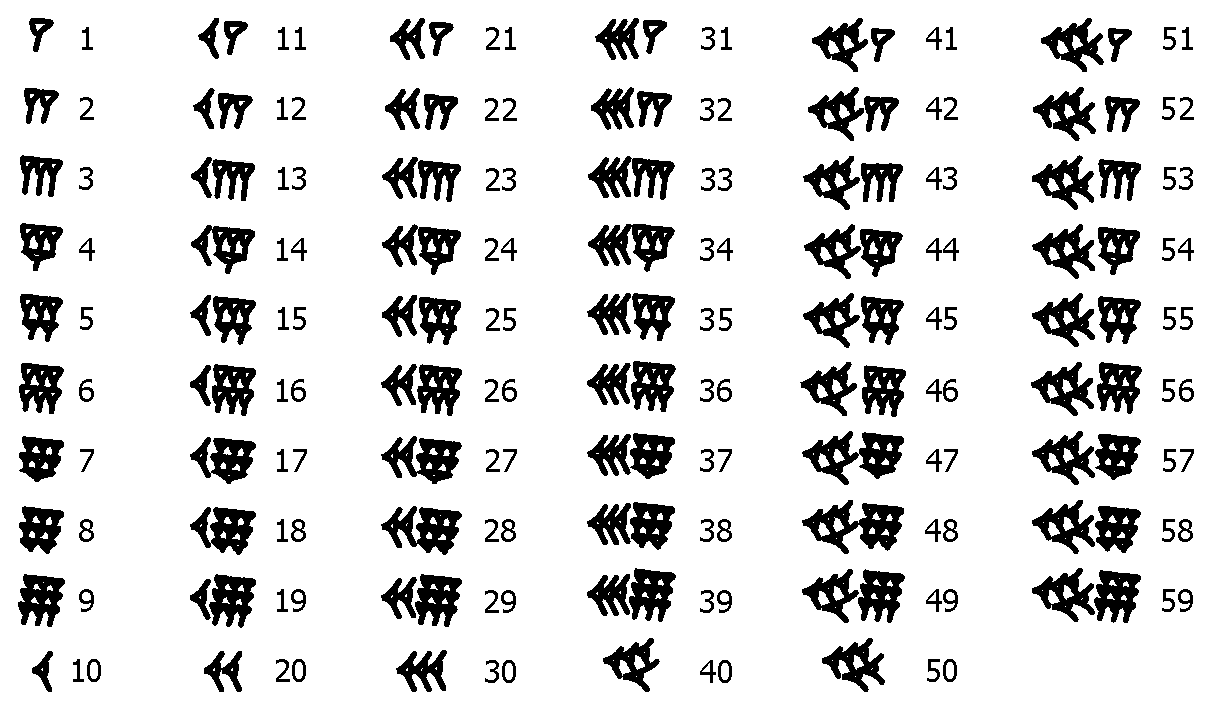
\includegraphics[width=0.9\marginparwidth]{../week1/figures/babylonian.eps}
\caption{The Ancient Babylonians counted using a number system based on the number sixty. They had sixty ``digits'' made using particular marks on cuneiform tablets. Can you imagine having to count with sixty numbers? That makes binary seem positively easy!\attribution{By Josell7, CC BY-SA 4.0, https://commons.wikimedia.org/w/index.php?curid=9862983}}
\label{fig:babylonians}
\end{marginfigure}

\begin{figure}[p]
  \label{fig:just-two} \centering \begin{tikzpicture} \begin{ttboard}[blue
  marbles=8] \TTBit[on]{3}{0} \TTBit[off]{3}{2}

      \TTRamp[right]{4}{1}
      \TTRampRun{4}{1}{\TTRows-2}

      \TTRamp[right]{2}{1}
      \TTInterceptor{2}{3}
    \end{ttboard}
  \end{tikzpicture}
  \caption{Here we have a two-bit machine, but we flipped the top bit so that it starts off pointing right. How many marbles are produced?}
\end{figure}

\subsection{Exploring the Binary Numbers}
\label{sec:binary-numbers}

You're probably familiar with the decimal numbers, which are the numbers we usually count with. The
decimal numbers use ten digits: 0, 1, 2, 3, 4, 5, 6, 7, 8, and 9. To write numbers larger than 9, we
use two digits.\curious{The word \emph{bit} is actually short for \emph{binary digit}.}

For example, to write the number one more than nine, we write ``10''. Then, to write the number one
bigger than that, we have a zero in the one's place, so we have more digits to use. The next digit
after 0 is 1, so the number after 10 is written as ``11''.

It works exactly the same in binary, except we only have two digits: 0 and 1. The binary number 0
means zero and the binary number 1 means one. But how do we write the number two? It's just like
writing the number ten in decimal. Since we don't have another digit, we use two digits. Two can be
written as ``10''.

\didyouknow{There are \emph{infinite} ways of representing numbers. Computer programmers commonly
  use decimal and binary and also two others, known as hexadecimal and octal. We'll cover these
  later.}  This system of using multiple digits to write out numbers for which we do not have enough
digits is called \term{place value}, because the position of the digits in the number representation
is what determines the value.

Let's think about how it works. First, consider some decimal (normal) numbers. We can write out any
two-digit decimal number as the sum of its ten part and its one part:

\[\begin{array}{rcl}
11 &=& 10 + 1. \\
25 &=& 20 + 5. \\
48 &=& 40 + 8.
\end{array}\]

The tens part can further be written as a product of a single digit and the number 10. The numbers
below have their digits colored so you can see where each digit ends up in the sum.

\[\begin{array}{rcl}
\textcolor{blue}{1}\textcolor{red}{1} &=& \textcolor{blue}{1} \times 10 + \textcolor{red}{1}. \\
\textcolor{blue}{2}\textcolor{red}{5} &=& \textcolor{blue}{2} \times 10 + \textcolor{red}{5}. \\
\textcolor{blue}{4}\textcolor{red}{8} &=& \textcolor{blue}{4} \times 10 + \textcolor{red}{8}.
\end{array}\]

What about three digit numbers? Well we can do the same thing, but we use 100 for the third digit, not 10.

\[\begin{array}{rcl}
\textcolor{green}{6}\textcolor{blue}{1}\textcolor{red}{1} &=& \textcolor{green}{6} \times 100 + \textcolor{blue}{1} \times 10 + \textcolor{red}{1}. \\
\textcolor{green}{8}\textcolor{blue}{2}\textcolor{red}{5} &=& \textcolor{green}{8} \times 100 + \textcolor{blue}{2} \times 10 + \textcolor{red}{5}. \\
\textcolor{green}{3}\textcolor{blue}{4}\textcolor{red}{8} &=& \textcolor{green}{3} \times 100 + \textcolor{blue}{4} \times 10 + \textcolor{red}{8}.
\end{array}\]

Of course 100 is just $10 \times 10$:

\[\begin{array}{rcl}
\textcolor{green}{6}\textcolor{blue}{1}\textcolor{red}{1} &=& \textcolor{green}{6} \times 10 \times 10 + \textcolor{blue}{1} \times 10 + \textcolor{red}{1}. \\
\textcolor{green}{8}\textcolor{blue}{2}\textcolor{red}{5} &=& \textcolor{green}{8} \times 10 \times 10 + \textcolor{blue}{2} \times 10 + \textcolor{red}{5}. \\
\textcolor{green}{3}\textcolor{blue}{4}\textcolor{red}{8} &=& \textcolor{green}{3} \times \underbrace{10 \times 10}_{\footnotesize \text{also written }10^2} + \textcolor{blue}{4} \times 10 + \textcolor{red}{8}.
\end{array}\]

We can do something similar for four-digit numbers:
\[\begin{array}{rcl}
\textcolor{orange}{3}\textcolor{green}{6}\textcolor{blue}{4}\textcolor{red}{1} &=& \textcolor{orange}{3} \times \underbrace{10 \times 10 \times 10}_{10^3} + \textcolor{green}{6} \times \underbrace{10 \times 10}_{10^2} + \textcolor{blue}{4} \times 10 + \textcolor{red}{1}. \\
\end{array}\]

As noted above, we can write out repeated multiplications of 10 with itself
as $10^2$, $10^3$, $10^4$.\curious{If $10^2 = 10 \times 10 = 100$ and $10^3 = 10 \times 10 \times 10 = 1000$ what is $10^1$?
  What about $10^0$?}

\[\begin{array}{rcl}
\textcolor{orange}{3}\textcolor{green}{6}\textcolor{blue}{4}\textcolor{red}{1} &=& \textcolor{orange}{3} \times 10^3 + \textcolor{green}{6} \times 10^2 + \textcolor{blue}{4} \times 10 + \textcolor{red}{1}. \\
\end{array}\]

To make the leap to binary numbers, we note that the number 10 is to decimal as the number 2 is to
binary.\curious{The number corresponding to place value number systems is called the
  \term{base}. ``Base 10'' is another way of saying decimal, and ``base 2'' is another name for
  binary.}

Consider the numbers above. We said the binary number ``110'' was decimal number 6. Let's apply the
same rules we did for decimal numbers to ``110''. First, we take each digit. Then we multiply each
digit by the number of twos corresponding to its position.

\curious{It is important to know what base we are dealing with when looking at a particular string
  of digits. In most mathematics, we assume that a number is written in decimal, but if we want to
  be explicit about it, we can write the base of any number in small letters after and below the
  number. For example, the number $110_{10}$ corresponds to the number one hundred and ten. The $10$
  below the $110$ signals that this number is in decimal. Similarly, the number $110_2$ corresponds
  to six.}
\[
\begin{array}{rcl}
  \textcolor{green}{1}\textcolor{blue}{1}\textcolor{red}{0} &=& \textcolor{green}{1} \times 2 \times 2 + \textcolor{blue}{1} \times 2 + \textcolor{red}{0} = 6, \text{or} \\
  \textcolor{green}{1}\textcolor{blue}{1}\textcolor{red}{0} &=& \textcolor{green}{1} \times 2^2 + \textcolor{blue}{1} \times 2 + \textcolor{red}{0} = 6, \text{or} \\
  \underbrace{\textcolor{green}{1}\textcolor{blue}{1}\textcolor{red}{0}}_{\text{in binary}} &=& \textcolor{green}{1} \times 4 + \textcolor{blue}{1} \times 2 + \textcolor{red}{0} = \underbrace{6}_{\text{in decimal}}
\end{array}
\]

This way of expanding numbers is very general and works for all
bases. Its often more convenient to write them out as tables. For
example, consider the decimal number $5837$. We can write it out as:

\hint{These are known as the places:
  the units place\tikzmarknode{week1unitsfrom}, \\
  the tens place\tikzmarknode{week1tensfrom},\\
  the hundreds place\tikzmarknode{week1hundredsfrom}, and \\
  the thousands place\tikzmarknode{week1thousandsfrom}.
}
\begin{center}
  \begin{tabular}{c|c|c|c}
    \hline
    \multicolumn{4}{c}{Place} \\\hline
    \tikzmarknode{week1thousandsto}3 & \tikzmarknode{week1hundredsto}2 & \tikzmarknode{week1tensto}1 & \tikzmarknode{week1unitsto}0 \\\hline
    $10^3$ & $10^2$ & 10 & 1 \\
    $\times$ & $\times$ & $\times$ & $\times$ \\
    5 & 8 & 3 & 7 \\\hline
    5000 + & 800 + & 30 +& 7= \\\hline
    \multicolumn{4}{c}{5837} \\\hline
  \end{tabular}
\end{center}
\tikzbackground{
  \draw[->, gray!20] (week1thousandsfrom.\tikztufteinner) to[bend left] (week1thousandsto.\tikztufteouter);
  \draw[->, gray!20] (week1hundredsfrom.\tikztufteinner) to[bend left] (week1hundredsto.\tikztufteouter);
  \draw[->, gray!20] (week1tensfrom.\tikztufteinner) to[bend left] (week1tensto.\tikztufteouter);
  \draw[->, gray!20] (week1unitsfrom.\tikztufteinner) to[bend left] (week1unitsto.\tikztufteouter);
}

Similarly, we can do the same for a binary number. Consider the \emph{seven-bit} binary number ``1101001'':
\didyouknow{A binary number that can be written in eight or fewer bits is known as a \term{byte}.}

\hint{Similarly, binary has place names corresponding to the numbers
  that are formed by repeatedly multiplying by two:
  the \ordinalnum{64} place\tikzmarknode{week164from},\\
  the \ordinalnum{32} place\tikzmarknode{week132from},\\
  the \ordinalnum{16} place\tikzmarknode{week116from}, \\
  the \ordinalnum{8} place\tikzmarknode{week18from},\\
  the \ordinalnum{4} place\tikzmarknode{week14from},\\
  the twos place, \tikzmarknode{week12from} and \\
  the units place \tikzmarknode{week11from}.}
\begin{center}
  \begin{tabular}{c|c|c|c|c|c|c}
    \hline
    \multicolumn{7}{c}{Place} \\\hline
    \tikzmarknode{week164to}6 & \tikzmarknode{week132to}5 & \tikzmarknode{week116to}4 & \tikzmarknode{week18to}3 & \tikzmarknode{week14to}2 & \tikzmarknode{week12to}1 & \tikzmarknode{week11to}0 \\\hline
    $2^6$ & $2^5$ & $2^4$ & $2^3$ & $2^2$ & 2 & 1 \\
    64 & 32 & 16 & 8 & 4 & 2 & 1 \\
    $\times$ & $\times$ & $\times$ & $\times$ & $\times$ & $\times$ & $\times$ \\
    1 & 1 & 0 & 1 & 0 & 0 & 1 \\\hline
    64 + & 32 + & 0 + & 8 + & 0 + & 0 + & 1 =\\\hline
    \multicolumn{7}{c}{105} \\\hline
  \end{tabular}
\end{center}
\tikzbackground{
  \draw[->, gray!20] (week164from.\tikztufteinner) to[bend right] (week164to.\tikztufteouter);
  \draw[->, gray!20] (week132from.\tikztufteinner) to[bend right] (week132to.\tikztufteouter);
  \draw[->, gray!20] (week116from.\tikztufteinner) to[bend right] (week116to.\tikztufteouter);
  \draw[->, gray!20] (week18from.\tikztufteinner)  to[bend right] (week18to.\tikztufteouter);
  \draw[->, gray!20] (week14from.\tikztufteinner)  to[bend right] (week14to.\tikztufteouter);
  \draw[->, gray!20] (week12from.\tikztufteinner)  to[bend right] (week12to.\tikztufteouter);
  \draw[->, gray!20] (week11from.\tikztufteinner)  to[bend right] (week11to.\tikztufteouter);
}

So the binary number $1101001_2$ corresponds to decimal $105_{10}$.

\begin{TryThisBox}
  Try translating the binary numbers below into the appropriate decimal number using the table and
  the summation methods described above:
  \begin{enumerate}
  \item $0_2$
  \item $10_2$
  \item $101_2$
  \item $111_2$
  \item $10111_2$
  \item $1111101_2$
  \item $10010001_2$
  \item $10000101_2$
  \end{enumerate}
\end{TryThisBox}

\section{From Marbles to Code}

\begin{marginfigure}
  \includegraphics[width=0.8\linewidth]{../week1/figures/alan-turing.jpg}
  \caption{\textbf{Alan Turing} (1912-1954) asked ``What can machines do if they follow
    rules''?. The name \emph{Turing Tumble} comes from Alan Turing. }
\end{marginfigure}

Inside a modern computer, tiny moving things called \emph{electrons} flow through parts that follow
simple rules, just like the pieces on the Turing Tumble board. Some parts remember things, some
parts make decisions, and some parts make sure electrons move in the right direction.

Binary numbers are fundamental to electronic computers because computers represent numbers as
electronic switches that are either on or off, which correspond to binary digits $0_2$ and
$1_2$. The computers you built above are \emph{real} computers, but building very large systems with
them would get complicated. That's why modern computers use electricity.

\begin{BigIdeaBox}
  Whether it uses marbles or electricity, a computer is just a system
  that follows rules.
\end{BigIdeaBox}

Modern computers are built so that you don't need to physically move
pieces to make them do new things. Instead, they can follow many
different rules depending on what you ask them to do.\curious{Every
  computer has a basic set of rules that depends on the physical parts
  inside it. Programming languages like Python are built on top of
  these rules, but we don't need to worry about them yet. This hidden
  layer of rules is sometimes called the \term{computer
    architecture}.}

The process of telling a computer which rules to follow is called \term{programming}. There are many
ways to program a computer. In the Turing Tumble game, we moved pieces physically. On modern
computers, we use something called a \term{programming language}.

One of the simplest programming languages to start with is called
\term{Python}.\aside{Don't worry, this kind of python does not bite! But it is made of bits and \emph{bytes}!}

\subsection{Talking to a Computer}

In this class, we will use the \textbf{Thonny} Python environment.
\aside{Thonny can be downloaded at \href{https://thonny.org}{https://thonny.org}.}

\begin{figure}
  \fixfigure
  \centering
  
\includegraphics[width=0.9\linewidth]{../week1/figures/thonny-interface.pdf}
  \caption{The Thonny interface. The interface is split into two
    parts: (1) the editor and (2) the prompt.}
  \label{fig:thonny-interface}
\end{figure}

We can talk to Python by entering ``rules'' into the prompt (see
\prettyref{fig:thonny-interface}) and immediately seeing what
happens. This is like dropping a marble into the machines we built
earlier and watching what happens.  \didyouknow{Long before modern
  computers, scholars attempted to study \emph{human} language through
  using rules. One such scholar was the Indian grammarian
  P\={a}\d{n}ini. Around 500 BC, he described the Sanskrit language
  using a precise set of rules that could combine to generate all
  valid sentences in that language!}

In Turing Tumble, our rules were made of plastic pieces. In Python, we
use special words and symbols to write rules.

Let's type our first rule! The simplest rules (also known as \term{expressions})
are the ones that stand for numbers. We can enter these rules by
typing in a number and pressing the Enter or Return key.

Try entering these into the Thonny prompt, and see what
happens.\hint{Type each line one at a time and observe what happens.}

\begin{replbox}
1<ENTER>
54<ENTER>
0<ENTER>
\end{replbox}
\hint{The response from the computer to each of these should be
  numbers. If it's not, you may have typed it in incorrectl. Try it
  again. If that still doesn't work, see \prettyref{sec:errors}}

The rule for numbers is that when you enter them in, you get the same
number out!

\begin{BigIdeaBox}
  Just like the ball thrown up in the air, and just like the
  machines we built, every time you run these rules, the answer is the
  same!
\end{BigIdeaBox}

Python understands many different kinds of numbers. By default, Python uses decimal numbers, as we'd
expect, but we can also use binary numbers. We write binary numbers by putting \code{0b} in front of
the number. Python will respond back in decimal.

\begin{replbox}
0b1<ENTER>
0b101<ENTER>
0b1101<ENTER>
\end{replbox}

We can also ask Python to write a decimal number in binary using \code{bin()}.

\hint{From now on, all the rules we see will be
    \emph{colored}. You don't need to enter the colors in. The colors
    only serve to make the rules easier to read. This is called
    \term{syntax highlighting}.}
\begin{replbox}
bin(10)<ENTER>
bin(1)<ENTER>
bin(2)<ENTER>
bin(3391249)<ENTER>
\end{replbox}

Let's try something more complicated. Before trying the following
rules, think about what is going to happen. A good programmer tries to
predict the output before they use the rule.  \curious{When you type
  something into Python and press Enter, the computer always produces
  the same result for the same input. This idea is called
  \term{determinism}.}

\begin{replbox}
1 + 1<ENTER>
5 - 3<ENTER>
4 * 3<ENTER>
\end{replbox}

\subsection{How Computers Follow Rules}

The symbols we used above connected two number rules together. When we
pressed enter, we got a new number, which is itself a kind of
rule. The way this number was generated depended on the exact symbol
we used. You're probably familiar with the \code{+} symbol, which
means addition. Can you guess what the \code{*} symbol stands for?
If you guessed multiplication, you're right. \hint{You're probably
  familiar with the symbol $\times$ for multiplication, but that
  symbol is hard to type! Most programming languages use \code{*} to
  denote multiplication.}

Since Python lets us combine rules however we want, we can combine
rules involving both multiplication and addition. Before trying the
exercises below, try to guess what the answer is and write down why.

\begin{replbox}
4 + 2 * 3<ENTER>
2 * 3 + 4<ENTER>
\end{replbox}

You may be surprised that the these rules both produced the same number.

In many programming languages, including Python, symbols like
\code{+} and \code{*} have rules to determine which one goes
first. In this case, multiplication always goes first.\curious{\term{Operator precedence} rules determine which written rules get done first.}

Sometimes it can help to \emph{draw} the expressions to figure out
exactly what is going on as in \prettyref{fig:parenrules}.

% TODO figure that shows how to make these into trees

What if we want to make additions occur first? We can always use
parentheses (that is \code{(} and \code{)}) around rules we want to
execute first.

\begin{replbox}
2 * 3 + 4<ENTER>
2 * (3 + 4)<ENTER>
\end{replbox}\hint{Remember it's always a good idea to \emph{predict} what is going to happen \emph{before} hitting the Enter key.}

In this case, the parentheses force the \code{3 + 4} rule to execute
first. \prettyref{fig:parenrules} shows how the diagram for this rule
looks different than the diagram for the \code{2 * 3 + 4} rule.

\begin{figure}
  \fixfigure
  \begin{minipage}{0.45\linewidth}
    \centering
    \begin{forest}
      [{*}
        [2]
        [{+} [3] [4]]]
    \end{forest}
  \end{minipage}
  \begin{minipage}{0.45\linewidth}
    \centering
    \begin{forest}
      [{+}
        [{*}
          [2]
          [3]]
        [4]]
    \end{forest}
  \end{minipage}
  \caption{The rule \code{2 * (3 + 4)} is drawn differently than the rule \code{2 * 3 + 4}.}
  \label{fig:parenrules}
\end{figure}

\begin{BigIdeaBox}
  When rules combine, there are rules to determine which rule go
  first. No matter which rules we are talking about, they always
  behave in \emph{exactly} the same way.
\end{BigIdeaBox}

There's one more thing to think about. What if we put parentheses around the
multiplication?\hint{It's always good to remember that computers don't think about \emph{why} they
  do something. They only know \emph{what} to do!}

\begin{replbox}
2 * 3 + 4<ENTER>
(2 * 3) + 4<ENTER>
\end{replbox}
\hint{At this point, you probably know you need to \emph{predict} what is going to happen before proceeding!}

In this case, it again helps to draw it out. As you can see both of
these rules can be represented by the same diagram (see
\prettyref{fig:paren-mult}). Since the diagrams match, the rules mean
the same thing even though they're typed out differently.
\curious{Electronic computers are structured as layers of rules. A
  really hard-working computer programmer made rules that told Python
  what to do to understand the rules you type in to the
  computer. Those rules were typed out in another language called
  C. Another program called a \term{compiler} took those rules and
  generated yet more sets of rules. Its rules all the way down!}

\begin{BigIdeaBox}
  The same rule can be typed out many different ways! We can apply the
  rules for diagramming rules to see if they mean the same
  thing.
\end{BigIdeaBox}

\begin{figure}
  \fixfigure
  \centering
  \begin{forest}
  [{+}
   [{*} [2] [3]]
   [4]]
  \end{forest}
  \caption{The rule \code{2 * 3 + 4} and \code{(2 * 3) + 4} are
    represented by the same diagram even though they are typed out
    differently.}
  \label{fig:paren-mult}
\end{figure}

\subsection{Rules with Words}

So far, all our rules have involved numbers, but computers can handle
more than that. Computers can also follow rules about
\emph{words}.\didyouknow{Python actually has \emph{two} kinds of
  numbers, but we will have to come back to that later.}

\begin{replbox}
"hello"<ENTER>
"my name is Bob"<ENTER>
\end{replbox}
\hint{Words must be surrounded by \code{"}s or you will get an
  error. Make sure you type everything in exactly as written.}

You'll notice that Python responds back with the word (or phrase) you
put in. \didyouknow{Programmers use the term \term{strings} to refer to
  rules representing words in programs.}

Now try this, but remember to \emph{predict} what is going to happen
before typing it in.\huh{But I thought
  \code{+} added numbers together. How come I can use it with
  words?}{Some symbols like \code{+} can do different things depending
  on whether it is used with words or numbers. Different programming
  languages have different rules regarding which combinations of
  simbols, words, and numbers are allowed and what exactly they
  mean. The technical term for this is \term{operator overloading}. A
  useful list of these rules in Python is given in
  \prettyref{tab:operator-rules-1}}

\begin{replbox}
"hello " + "world"<ENTER>
\end{replbox}

Did it do what you expected? If you typed it in correctly, Python
should have responded with \code{"hello world"}.

We've now seen a rule involving words! When you use \code{+} on two
words, you get those two words put together. What else can we do with words?

\begin{replbox}
"ho" * 3<ENTER>
\end{replbox}

You should see the response \code{"hohoho"}, which is just \code{"ho"}
repeated three times. \hint{Python did not suddenly decide to be
  festive. The word returned is the result of Python applying its set
  of rules \emph{exactly} to what you wrote.}

\begin{TryThisBox}
Can you multiply a word by another word? What would this mean? Think
about it, before we find out the answer in the next section.
\end{TryThisBox}

\begin{marginfigure}
  \centering
  \includegraphics[width=0.9\marginparwidth]{../week1/figures/game-of-life.png}
  \caption{The Game of Life by John Conway is a system that follows simple rules that can create complex behavior. Above is an example of expressing a rule in the Game of Life. See the Deep Dive Box on page \pageref{box:gameoflife} for more information.\attribution{Hyperdeath, CC BY-SA 3.0 <https://creativecommons.org/licenses/by-sa/3.0>, via Wikimedia Commons}}
\end{marginfigure}

\subsection{Some Rules Don't Make Sense}
\label{sec:errors}

Remember that when we type rules, Python applies more rules to make
sense of what we typed. We can visualize these rules by drawing
diagrams. But sometimes, we write something that Python's rules cannot
figure out. Although we can type them using the keyboard they don't
make sense to Python. This would be like trying to place two Turing
Tumble pieces on one peg when building a machine -- it just doesn't
make sense. We call these issues \term{syntax errors}.

\begin{replbox}
2 + 5 +<ENTER>
* 4<ENTER>
\end{replbox}

Other times we type rules that Python understand, but when it tries to
process them, it gets confused. This is like placing a much larger
marble into the Turing Tumble game -- although our placement of pieces
makes sense, we cannot make the pieces move with the wrong type of
marble. This is called a \term{runtime error}. You may have also heard
it called a \term{bug}. \didyouknow{The first computer bugs were
  caused by actual bugs that got stuck in hot electronic parts used in
  the earliest electric computers. Yuck!}

Both of these issues are kinds of \term{errors}.

\begin{BigIdeaBox}
  Python always applies the same rules to understand and process our
  rules, but sometimes what we put in doesn't make sense.
\end{BigIdeaBox}

In Python, errors are reported back to us as they occur, and Python
tries to give us information that can help us correct the error.
\hint{Although it may seem scary, there is nothing ``wrong'' with an
  error. It's just the computer applying rules and telling you
  something doesn't make sense.}

Although Python will provide some information that can be useful to
fix our program, Python is itself a collection of rules, and its rules
may not fully understand what we are trying to do based on what we
input. This is where the job of a programmer becomes important.

See \prettyref{tab:python-errors} for examples of some errors we
might encounter as we continue with our learning. You don't need to
memorize these, but it may be useful to refer back.

\begin{table}
  \fixfigure

\begin{tabularx}{\linewidth}{lp{0.6\linewidth}}
\toprule
\code{NameError} & A name of a rule was mistyped (i.e., you typed \code{length} instead of \code{len}). \\
\code{TypeError} & You used a number where a word was expected or vice versa (i.e., \code{'hello'/2}). \\
\code{ZeroDivisionError} & You tried to divide a number by zero. Uh-oh! \\
\code{SyntaxError} & Python couldn't make sense of what you typed because it didn't follow Python's rules (i.e., you typed \code{2 + 5 *} and python doesn't know what to multiply 5 by). \\
\code{OverflowError} & Some kinds of calculations on numbers can result in very large numbers that don't fit into the computer. \\\bottomrule
\end{tabularx}

\caption{As we continue in our learning, we will most likely encounter more errors. Errors are a
  \emph{normal} part of programming. They do not mean anything is broken! It just means there's been
  a misunderstanding between what you thought was going to happen and what actually happened when
  the computer followed through exactly with the rules you set out for it. Instead of being
  discouraged, think of every error as an opportunity learn \emph{more}!}
\label{tab:python-errors}
\end{table}

\section{Conclusion}

Computers follow rules exactly. When we program a computer, we make
new rules for the computer to follow. In Python, simple rules can
involve numbers and words. Sometimes, the rules we write don't make
sense. This is called an error, but is still the result of the
computer following a set of rules.

We haven't learned how to program \emph{yet}, but we have started
toying with the idea of turning ideas into instructions. When we do
this, the small details really matter. Missing pieces can cause
confusion. Unclear instructions lead to unexpected results. When
things go wrong, it's not because the computer was wrong, but because
it followed the instructions exactly as written.

This is computer's greatest strength. They never guess or fill in
missing steps. They just do exactly what you tell it! Computer science
is not about memorizing commands or tying a lot. It's about learning
how to say things clearly enough that a process -- whether a table
game, machine, or a person -- can follow your ideas without confusion.

In the next chapter we'll start to think deeper about how to precisely
describe to the computer the things we want to make.

\begin{DeepDiveBox}
  \boxtitle{Simple Rules, Surprising Worlds: The Game of Life}
  \label{box:gameoflife}

  One of the most famous rule-based systems ever created is called the \emph{Game of Life}, invented
  by mathematician John Conway.

  Despite the name it isn't really a game -- it's a world that follows rules.

  Imagine a giant sheet of graph paper. Each square can either be \emph{alive} or
  \emph{dead}. That's it. No colors, no thinking, nothing. Just alive or dead.
  \margmark{play-life}{\curiousboxtext You can play the game of life by going to \href{https://playgameoflife.com}{https://playgameoflife.com}.\\
    \begin{center}
      \qrcode{https://playgameoflife.com}
  \end{center}}

  The game proceeds in turns. At each turn, each square looks at its eight neighbors and follows
  these simple rules (all squares update at the same time):
  \begin{enumerate}
  \item If a square is \emph{alive} and has fewer than two live neighbors, it gets lonely and dies.
  \item If a square is \emph{alive} and has two or three live neighbors, it stays alive.
  \item If a square is \emph{alive} and has more than three live neighbors, it suffocates and dies.
  \item If a square is \emph{dead} and has exactly three live neighbors, it comes to life.
  \end{enumerate}
  \margmark{gameofliferules}{
      Each turn, a cell looks at its neighbors and decides to either come to life, stay alive, or die. \\
      \begin{tikzpicture}
        \foreach \x in {0,1,2} {
          \foreach \y in {0,1,2} {
            \draw (\x,\y) rectangle ++(1,1);
          }
        }
        \fill[red] (1,1) rectangle ++(1,1);
        \node [anchor=south west] at (0, 2) {1}; % top-left
        \node [anchor=south west] at (1, 2) {2}; % top-middle
        \node [anchor=south west] at (2, 2) {3}; % top-right
        \node [anchor=south west] at (0, 1) {4}; % middle-left
        \node [anchor=south west] at (2, 1) {5}; % middle-right
        \node [anchor=south west] at (0, 0){6}; % bottom-left
        \node [anchor=south west] at (1, 0) {7}; % bottom-middle
        \node [anchor=south west] at (2, 0) {8}; % bottom-right
      \end{tikzpicture}
    }

  \textbf{\sffamily \large What Happens?}

  Surprisingly, this system is a \emph{full} computer and can compute \emph{anything}. You can build
  patterns that do all sorts of things. Some patterns move across the board. Some repeat
  forever. Some patterns build other patterns.

  All of this comes from just four simple rules!

  The Game of Life shows something very important: \textbf{Simple rules can create behavior that
    looks alive, planned, or intelligent -- even when nothing is thinking}. This is the same idea
  behind the electronic computers that we use every day.
\end{DeepDiveBox}

\Exercises

\curious{Exercises are fun things you can try at home}

\begin{exercises}
\item Construct Turing Tumble boards that do the following:
  \begin{enumerate}
  \item Construct an alterating sequence of marbles \ttpieces{rbrbrbrb}\ldots?
    \answer{}
  \item Returns a sequence of alternating marbles one red, two blue like \ttpieces{rbbrbbrbb}\ldots?
  \item In class, we built boards to count out a number of marbles. We used sequences of bits to do
    this. These sequences are known as \emph{registers}. Can you build a board that takes a binary
    number in a register and \emph{adds one} to that binary number?
  \item Can you extend the board you made above to contain two separate registers and have the board
    add the two binary numbers together? Try one-bit and two-bit registers. What limits do you run
    up against as you try to increase the number of bits?
  \end{enumerate}

\item Figure out the rule that the following Turing Tumble boards follow when a blue ball is released first:
  \begin{tasks}(2)
  \task \answer{It produces one blue marble and then all the red marbles}
    \begin{tikzpicture}[baseline=(ttboardtop.base)]
    \begin{ttboard}[margin, blue marbles=5, red marbles=5, blue marbles released=1, output={\Large ?}]
      \TTRamp[right]{3}{0}
      \TTRamp[left]{7}{0}
      \TTRamp[right]{4}{1}
      \TTRamp[left]{6}{1}
      \TTRamp[right]{5}{2}
      \TTRamp[right]{6}{3}
      \TTRamp[right]{7}{4}
      \TTRampRun{8}{5}{\TTRows - 2}
    \end{ttboard}
    \end{tikzpicture}

  \task \answer{It produces an alternating run of marbles \ttpieces{brbrbrb}\ldots}
    \begin{tikzpicture}[baseline=(ttboardtop.base)]
      \begin{ttboard}[margin, blue marbles=5, red marbles =5, blue marbles released=1, output={\Large  ?}]
        \TTRamp[right]{3}{0}
        \TTRamp[left]{7}{0}
        \TTRamp[right]{4}{1}
        \TTRamp[left]{6}{1}
        \TTCrossover{5}{2}
        \TTRampRun{3}{3}{\TTRows - 2}
        \TTRampRun{6}{3}{\TTRows - 2}
      \end{ttboard}
    \end{tikzpicture}

  \task \answer{It produces an alternating run of marbles \ttpieces{brbrbrb}\ldots}
    \begin{tikzpicture}[baseline=(ttboardtop.base)]
      \begin{ttboard}[margin, blue marbles=5, red marbles =5, blue marbles released=1, output={\Large ?}]
        \TTRamp[right]{3}{0}
        \TTRamp[left]{7}{0}
        \TTRamp[right]{4}{1}
        \TTRamp[left]{6}{1}
        \TTBit{5}{2}
        \TTRamp[left]{4}{3}
        \TTRamp[right]{6}{3}
        \TTRampRun{3}{4}{\TTRows - 2}
        \TTRampRun{6}{4}{\TTRows - 2}
      \end{ttboard}
    \end{tikzpicture}

  \task \answer{It produces four blue marbles and then only red marbles.}
    \begin{tikzpicture}[baseline=(ttboardtop.base)]
      \begin{ttboard}[margin, blue marbles=5, red marbles =5, blue marbles released=1, output={\Large ?}]
        \TTBit[on]{3}{0}
        \TTBit[on]{3}{2}
        \TTRampRun{1}{1}{\TTRows - 2}
        \TTRamp[left]{4}{1}
        \TTRamp[right]{4}{3}
        \TTRamp[right]{5}{4}
        \TTRamp[right]{6}{5}
        \TTRamp[left]{7}{6}
        \TTRamp[left]{7}{0}
        \TTRamp[right]{6}{1}
        \TTRamp[right]{7}{2}
        \TTRamp[left]{8}{3}
        \TTRamp[left]{7}{4}
        \TTRamp[left]{6}{5}
        \TTBit[off,gear]{5}{6}
        \TTGear{4}{6}
        \TTBit[off,gear]{4}{7}
        \TTRamp[left]{6}{7}
        \TTRamp[right]{5}{8}
        \TTRamp[right]{6}{9}
      \end{ttboard}
    \end{tikzpicture}
  \end{tasks}
\item Predict the answer to the following Python rules:
  \begin{enumerate}
  \item \code{1 \enterkey}\answer{1}
  \item \code{-1 \enterkey}\answer{-1}
  \item \code{3 + 2 \enterkey}\answer{5}
  \item \code{3 * 9 + 6 \enterkey}\answer{35}
  \item \code{6 * 3 * 2 \enterkey}\answer{36}
  \item \code{6 + 3 + 2 \enterkey}\answer{11}
  \item \code{6 * 4 - 8 * 2 \enterkey}\answer{8}
  \item \code{6 * 4 // 2 \enterkey}\hint{Remember that \code{//} means division in Python}\answer{12}
  \end{enumerate}

\item Try the following rules.
  \begin{enumerate}
  \item \code{len(``a'')}
  \item \code{len(``ab'')}
  \item \code{len(``abc'')}
  \item \code{len("")}
  \end{enumerate}
  What does the \code{len} rule do?
  \answer{It calculates how many letters are in the word.}
\end{exercises}

\begin{table*}
  \begin{tabularx}{\linewidth}{llL}
      \toprule
      \headercol{Symbol} & & \headercol{Meaning} \\\midrule
      {\ttfamily *, //, \%} & \code{number * number} & Multiply two numbers together \\
      & \code{number // number} & Divide two numbers \\
      & \code{number \% number} & The remainder when dividing the numbers \\
      & \code{word * number} & Repeat the word this many times \\\hline
      {\ttfamily +, -} & \code{number + number} & Add two numbers together \\
      & \code{number - number} & Subtract the second number from the first \\
      & \code{word + word} & Combine the two words together \\
      \code{len} & \code{len(word)} & Get the number of letters and digits in the word \\
      \code{bin} & \code{bin(number)} & Get the binary number corresponding to the number \\\bottomrule
  \end{tabularx}
  \caption{This is a list of symbols you can use to combine rules in
    Python. Symbols that appear first are executed first, unless you
    use parentheses to force some rules to ge first. The behavior of
    symbols can depend on whether it's used with numbers or words. All
    these variants are given here}
  \label{tab:operator-rules-1}
\end{table*}

% -*- mode: latex -*-

\week{Data}

Get out a piece of paper and draw a duck. It can be any kind of duck you want, in whatever pose.

Once you're done, have your friend take out a new sheet of paper. Without showing them your drawing,
describe exactly what you drew and have them attempt to replicate it.

How did they do? If you're like most people, you probably gave directions that were vague enough to
be interpreted in many ways. Your friend's drawing probably doesn't look a whole lot like yours.

\begin{marginfigure}
  \centering
  \includegraphics[width=0.8\marginparwidth]{../week2/figures/duck.jpg}
  \caption{Can you describe exactly how to draw this duck? Your computer can!}
\end{marginfigure}

In casual conversation, we often mix up our own ideas of how things ought to be with the way things
are. None of the instructions you gave about how to draw your duck were wrong, and the drawing your
friend made from them is also not wrong. They just highlight different parts of how \emph{you}
interpreted your own drawing and how \emph{they} interpreted your description of it.\didyouknow{Many of the products we use today are
  made by computers that manipulate real life materials, like wood,
  metals, and plastic. Precise instructions are provided to these
  machines using a special computer unit called a \term{Computer
    Numerical Control} (or \term{CNC} module) that produce highly-detailed pieces like the one shown here.
  \vspace{0.6em}

  \includegraphics[width=0.8\marginparwidth]{../week2/figures/cnc-machine.jpg}
  \attribution{Cameronm125, CC BY-SA 4.0 <https://creativecommons.org/licenses/by-sa/4.0>, via Wikimedia Commons}
  }

When it comes to computers, we have to describe things exactly, because computers simply follow
rules. If the instructions you gave your friend were not clear, your friend probably figured out a
meaning that made sense to them. Computers don't do that. They simply do exactly as they are told.

\section{Week 1 Review}c

Last week, we discussed how certain machines obey rules. Once the rules were set up, the machine
always obeyed those rules. The machines we constructed counted marbles. We controlled how many
marbles came out by manipulating switches on a board.

Computers also use switches to count. Each switch in a computer can be on or off, or a ``1''
or ``0''. Every number can be written as 1s and 0s.

All of these principles are based on fixed rules.

We saw that Python also follows rules. We learned that Python can manipulate numbers and
words. Although numbers are stored internally in a binary form, Python interprets them for us, so
that we talk to it using the numbers we're familiar with. Python has rules for converting
numbers back into binary form and also for manipulating words.

\section{Drawing a Very Precise Duck}

\begin{marginfigure}
  \centering
  \begin{tikzpicture}
    \draw (0,0) pic[duck/water=blue] {duck};
  \end{tikzpicture}
  \caption{This is a very precise duck!}
  \label{fig:precise-duck}
\end{marginfigure}

Think back to the duck exercise we did at the beginning of class. We found it was hard to describe a
duck perfectly to our friend. That wasn't because we didn't know what a duck is -- it's because we
had no way to describe it precisely.

\begin{BigIdeaBox}
English is a great language for everyday communication, but it is not great at being exact about
visual information. To talk about drawings, we need a language that allows us to be precise about
something.
\end{BigIdeaBox}

Whenever we want to describe something in detail, we have to understand how to be precise about
it. Switches are precise -- they are either on or off. Numbers are precise too, because they can be
represented by a bunch of switches. We need a way of describing images in a similar manner.

%\begin{marginfigure}
%  \centering
%  \includegraphics[width=0.8\marginparwidth]{../week2/figures/plato.jpg}
%  \caption{The Greek philosopher \textbf{Plato} believed that things
%    existed before being described.}
%\end{marginfigure}

% \begin{TrackBox}{Gaming}
%   Some computer scientists try to match the descriptions and names on
%   the computer match those they observe in the real world. When we do
%   this, we can use the computer to predict what would happen. This is
%   called a \term{simulation}.
% \end{TrackBox}

\begin{bookbox}[p]
  \fixfigure
\label{box:pixels}
\begin{TrackBox}{Graphics}
  \boxtitle{How Computers Draw}

Computers draw using -- you guessed it -- numbers! You've probably seen the \term{number line} in
your math courses. All numbers can be placed on a simple line, and we can name any point on the line
by writing down a number to name it.

%\makemargmark{number line
%  comment}{\notestyle \huhnote{This coordinate system looks different than my math courses! What's
%    going on?}{If you've done geometry you've probably seen the cartesian plane drawn with the $y$
%    coordinate increasing as you go up. On many computers, the $y$ coordinate increases as you go
%    \emph{down}. Computers often use this different coordinate system so that the coordinates match
%    how things are physically drawn. It doesn't matter which system you choose, as long as everyone
%    does it the same way. In both systems, each grid is named by a unique number.}}

But to make graphics, we need to be able to talk about \tikzmarknode{points on a screen}{points} on
a rectangular screen, not a line. How do we name a point on a rectangle? The first person to think
about this systematically was a scientist, mathematician, and philosopher named \textbf{Ren\'e
  Descartes} who invented \emph{Cartesian plane}. Here's how it works. Instead of a line, we draw a
grid. We number all the columns and all the rows (see \prettyref{fig:cartesian-grid}). Now, any
square on the grid can be named by giving two numbers. These two numbers together are called the
\term{coordinate}. We usually write the \emph{column} number first, and the \emph{row} number
last. This system is called the \emph{cartesian coordinate} system.

\emph{Everything} you see on your screen is the result of your
computer following rules that turn lights on or off (see
\prettyref{fig:pixels}). Even the text you read is created by following
rules (known as \term{fonts}) that specify how to turn on a pattern of
lights to create the letter shapes.

The drawing library we are using in class translates the functions
you use into rules that turn on the right lights. Can you think of
how you might write some rules to draw some of the shapes below?

\tryitsection

Here are some problems to think about.

\begin{enumerate}
\item Which pixels would you turn on to draw a line between
  coordinate $(5, 2)$ and $(8, 5)$?
\item What about $(5,2)$ and $(9,0)$?
\item If someone gave you two coordinates $(x_1, y_1)$ and $(x_2,
  y_2)$ could you come up with a rule that determined which lights
  to turn on to draw a line? Try listing out the instructions
  \emph{exactly}.
\item Can you use the rule above to draw a triangle?
\item How would you draw a \emph{circle} around the point $(3, 8)$?
\end{enumerate}
\end{TrackBox}
\end{bookbox}
\onfloatpage{box:pixels}{
  \makemargmark{points on a screen}{
    % Requires:
% \usepackage{tikz}
% \usetikzlibrary{calc}

\begin{tikzpicture}[
  font=\sffamily,
  x=0.55cm, y=0.55cm, % pixel size
  line join=round
]
  % ---- grid size ----
  \def\W{12} % number of columns
  \def\H{12} % number of rows

  % ---- background ----
  \fill[white] (0,0) rectangle (\W,\H);

  % ---- draw grid ----
  \draw[step=1, gray!55] (0,0) grid (\W,\H);

  % ---- axis labels: x left->right, y top->bottom ----
  % Column indices along top: 0..W-1
  \foreach \x in {0,...,11} {
    \node[anchor=south, scale=1.1, font=\bfseries\sffamily, inner sep=1pt] at (\x+0.5, \H) {\x};
  }
  % Row indices along left, with y increasing downward:
  % Put 0 at the top row (near y=H-0.5), then 1 below it, ...
  \foreach \y in {0,...,11} {
    \node[anchor=east, scale=1.1, font=\bfseries\sffamily, inner sep=1pt] at (0, \H-\y-0.5) {\y};
  }

  % Optional axis titles
  \node[anchor=west, scale=0.8] at (0, \H+0.9) {x (columns)};
  \draw[->,line width=0.8pt] (2cm, \H+0.9) -s (\W,\H+0.9);
  \node[anchor=east, scale=0.8, rotate=90] at (-0.9, \H) {y (rows, down)}; % name this node Y
  \draw[->,line width=0.8pt] (-0.9, \H+4cm) -- (-0.9, 0); % start this at the south of Y offset by 0.5 downwards and continue it down

  % ---- helper: draw a pixel at (x,y) where y=0 is top row ----
  % We'll just place rectangles manually using the mapping:
  % pixel (x,y) -> rectangle from (x, H-y-1) to (x+1, H-y)

  % Colors
  \definecolor{petal}{RGB}{232,110,140}
  \definecolor{center}{RGB}{248,200,70}
  \definecolor{stem}{RGB}{70,160,90}
  \definecolor{leaf}{RGB}{90,190,110}

  % ---- flower pixels ----
  % petals (a chunky 5x5-ish flower head)


  % Petals (explicit, simpler)
  \foreach \x/\y in {
    5/2, 6/2,
    4/3, 7/3,
    3/4, 8/4,
    4/5, 7/5,
    5/6, 6/6,
    5/4, 6/4, 4/4, 7/4 % make it fuller
  }{
    \fill[petal] (\x, \H-\y-1) rectangle (\x+1, \H-\y);
  }

  % center
  \foreach \x/\y in {5/4,6/4,5/5,6/5} {
    \fill[center] (\x, \H-\y-1) rectangle (\x+1, \H-\y);
  }

  % stem
  \foreach \x/\y in {5/7,5/8,5/9,5/10} {
    \fill[stem] (\x, \H-\y-1) rectangle (\x+1, \H-\y);
  }

  % leaves
  \foreach \x/\y in {4/9,3/9,6/9,7/9} {
    \fill[leaf] (\x, \H-\y-1) rectangle (\x+1, \H-\y);
  }

  % ---- optional: outline the flower pixels slightly darker ----
  \foreach \x/\y in {
    5/2, 6/2,
    4/3, 7/3,
    3/4, 4/4, 5/4, 6/4, 7/4, 8/4,
    4/5, 5/5, 6/5, 7/5,
    5/6, 6/6,
    5/7,5/8,5/9,5/10,
    4/9,3/9,6/9,7/9
  }{
    \draw[black!35, line width=0.2pt] (\x, \H-\y-1) rectangle (\x+1, \H-\y);
  }

\end{tikzpicture}

 \par
    \captionof{figure}{Just like we can refer to any point on a line by
      a number, we can refer to any point on a rectangle or grid using
      two numbers. In this image of a flower, we can use cartesian
      coordinates to reference any square and change its color or turn
      it on or off.}
    \label{fig:cartesian-grid}
  }
}

\subsection{Drawing Our First Image}

In order to draw on a computer, we have to first think about what sort of \emph{language} we need to
use to be specific about what to draw. Once such language is called Turtle.

Turtle works by following -- you guessed it -- rules! Turtle works like an Etch-a-sketch. You supply
instructions that move a pen around a page. Turtle draws a line as the pen moves.

\begin{marginfigure}
  \centering
  \includegraphics[width=0.9\textwidth]{../week2/figures/Jack_of_hearts.jpg}
  \caption{The Turtle language works like an Etch-a-sketch. A pen moves around the page leaving marks that turn into images, such as this one.\attribution{By Etcha - Own work, CC BY-SA 3.0, https://commons.wikimedia.org/w/index.php?curid=5395767}}
  \label{fig:etchasketch}
\end{marginfigure}

% TODO Setup course materials

We're going to use a version of Turtle that is a bit more intuitive than ``standard'' Turtle. This
is provided as part of the course materials in the form of a \term{module}, which is a re-usable
bundle of Python code. In order to use this version, we will have to load it into Python. We can do
this with the \kw{import} rule.

We don't need to know all the details to use it. \curious{Check out \prettyref{fig:import} for a
  complete rundown of \kw{import}.} Let's go ahead and load Turtle and draw our first shape: a line.

\begin{figure}[b]
  \centering
  \begin{minipage}{0.9\textwidth}
    \Large \ttfamily
    \vspace{1.5cm}
    \begin{tcolorbox}[sharp corners]
      \tikzmarknode{importkw}{\kw{import}} \tikzmarknode{import module name}{week2.draw} \tikzmarknode{aspart}{\kw{as} draw}
    \end{tcolorbox}
    \vspace{3cm}
    \begin{tcolorbox}[sharp corners]
      \tikzmarknode{fromkw}{\kw{from}} \tikzmarknode{from import module name}{week2.draw} \tikzmarknode{import from}{\kw{import}} \tikzmarknode{import from star}{*}
    \end{tcolorbox}
  \end{minipage}
  \begin{tikzpicture}[remember picture, overlay]
    \node[above] (importkwnote) at ($(importkw) + (1cm, 1.5cm)$) {
      \begin{tcolorbox}[code note]
        \footnotesize \sffamily
        The \kw{import} rule tells Python to start loading a module.
      \end{tcolorbox}
    };
    \node[below] (import module name note) at ([xshift=-1cm, yshift=-1cm]import module name.south) {
      \begin{tcolorbox}[code note]
        \footnotesize \sffamily
        This is the name of the ruleset or \term{module} we want to use.
      \end{tcolorbox}
    };
    \node[anchor=north west] (aspartnote) at ([yshift=-0.6cm]aspart.south west) {
      \begin{tcolorbox}[code note, width=5cm]
        \footnotesize \sffamily
        This \emph{names} the module. We can refer to rules in the
        module as \code{draw.rule}. You can also ignore the \kw{as}
        part, and use the full name \code{week2.draw.rule}.
      \end{tcolorbox}
    };
    \draw[->, ultra thick] (importkwnote.south) to[in=90,out=-90] ([yshift=1em]importkw.north);
    \draw[->, ultra thick] (aspartnote.north) to[in=-90,out=90] (aspart.south);
    \draw[->, ultra thick] ([yshift=0.2ex]import module name note.north) to[in=-90,out=90] ([yshift=-0.5em]import module name.south);
    \draw[->, ultra thick] ([yshift=-0.2ex]import module name note.south) to[in=90,out=-90] ([yshift=2em]from import module name.north);
  \end{tikzpicture}
  \caption{The \kw{import} rule in Python lets you use extra sets of functionality that are not
    built-in to Python. It takes the name of a module, which is a series of words, separated by
    dots. You also specify how you want to refer to the rules contained in that module, after
    \kw{as}. If you don't include \kw{as}, you have to use the full name of the module.

    You can also get all the rules from a module using the \kw{from} / \kw{import} rule.
  }
  \label{fig:import}
\end{figure}

\begin{replbox}
>>> (*@\tikzmarknode{import keyword}{\kw{import}}@*) week2.draw as (*@\tikzmarknode{week2 draw name}{draw}@*)<ENTER>
>>> draw.draw(draw.forward(100))<ENTER>
\end{replbox}

What happened here? The pen started in the middle of the page, and then went \emph{forward} by 100
units.\curious{The units used by Turtle are called \term{pixels}. See \prettyref{fig:pixels} for
  more information} In this case, the pen always starts pointed to the right. So when we go forward,
turtle draws a line to the right.

Let's break it down further though. There are actually \emph{two} rules being used here. The first
is \code{draw.draw}. This rule takes a drawing and draws it. It doesn't draw anything on its own. If
you just did the following, you'd get a blank screen:

\begin{replbox}
>>> draw.draw()<ENTER>
\end{replbox}

You need to make a drawing in order for \code{draw.draw} to do something. This is what the
\code{draw.forward} rule does. Go ahead and try this:

\begin{replbox}
>>> draw.forward(10)<ENTER>
[('forward', 10)]
\end{replbox}

That didn't draw anything! That's because the \code{draw.forward} rule only describes \emph{what} to
draw. It doesn't do any drawing yourself. You need to ask Python to draw the drawing you create.

Now that we understand the difference between doing the drawing and planning the drawing, let's talk
about what we can do with the plans.

The simplest thing we can do with drawing plans is to combine them together in sequence -- first
make one drawing, then the other. You can put drawings together by using \code{+}, just like you can
with numbers. Let's try this:

\begin{replbox}
>>> draw.forward(10) + draw.turn('right') + draw.forward(20)<ENTER>
[('forward', 10), ('right', 90), ('forward', 20)]
\end{replbox}

Again, that's just the \emph{plan} for the drawing. It doesn't \emph{do} anything until you draw
it. Let's try drawing it:

\hint{For a full explanation of \code{draw.turn}, see \prettyref{deepdive:draw-turn-angles}}
\begin{replbox}
>>> draw.draw(draw.forward(10) + draw.turn('right') + draw.forward(20))<ENTER>
\end{replbox}

That's more like it.

What we saw above is the distinction between \term{data} and
effects. Data is information about something. Data describes what
something is. The \code{draw.forward} and \code{draw.turn} rules made
\emph{data}. The \code{draw.draw} rule used that data to make a
drawing.\didyouknow{The difference between data and effects is similar
  to the difference between \emph{nouns} and \emph{verbs}. Nouns don't
  do anything on their own. They're just there. You need a verb to do
  something with it.}

\subsection{More Complex Drawings}

\curious{For a full list of all the Turtle rules we can use see \prettyref{tab:turtle}.}
Let's try changing the pen color using the \code{draw.color} rule.

\hint{For a sample list of colors we can use, see \prettyref{fig:turtlecolors}}
\begin{replbox}
>>> draw.draw(draw.color('blue')+draw.forward(100))<ENTER>
\end{replbox}

Did it do what you thought it would?

You've seen how to turn the pen above to draw a corner. We can go ahead and extend that to draw a square.

\begin{marginfigure}
  \centering
  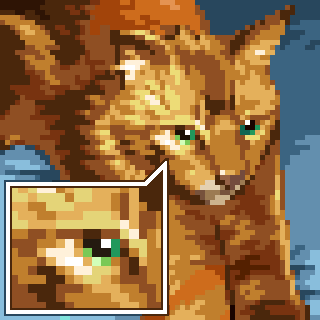
\includegraphics[width=0.9\marginparwidth]{../week2/figures/CatPixels.pdf}
  \caption{Every image you see on a computer screen is made up of tiny lights called \term{pixels}
    arranged in a grid. If you carefully look at your computer screen, you may be able to see the
    individual pixels. By turning the lights on and off and adjusting the color, the computer can
    display any image, such as this one of a cat.  \attribution{Original: ReffPixels?Vector:
      OmegaFallon, CC BY-SA 4.0 <\url{https://creativecommons.org/licenses/by-sa/4.0}>, via
      Wikimedia Commons}}
  \label{fig:pixels}
\end{marginfigure}

\tikzforeground{
  \node (repl dots hint) at ($(repl dots.north east) + (8cm, 2cm)$) {
    \begin{tcolorbox}[code note]
      If we don't complete our rule on the \code{{>}{>}{>}} line, Python will respond with these dots to
      ask us to complete the rule. It tries to be nice that way!
    \end{tcolorbox}
  };
  \draw[->] (repl dots hint.south) to[in=-20,out=-90,looseness=0.6] (repl dots.south east);
}
\begin{replbox}
>>> draw.draw(draw.color('blue') +
...  draw.forward(100) +
...  draw.turn('right') +
...  draw.forward(100) +
...  draw.turn('right') +
...  draw.forward(100) +
...  draw.turn('right') +
(*@\tikzmarknode{repl dots}{...}@*)  draw.forward(100))<ENTER>
\end{replbox}

Phew! That was a lot of typing! If we had to do that everytime we wanted to draw a square, we would
have to write \emph{a lot} of \emph{rules}.

\begin{figure}[b] 
  \centering
  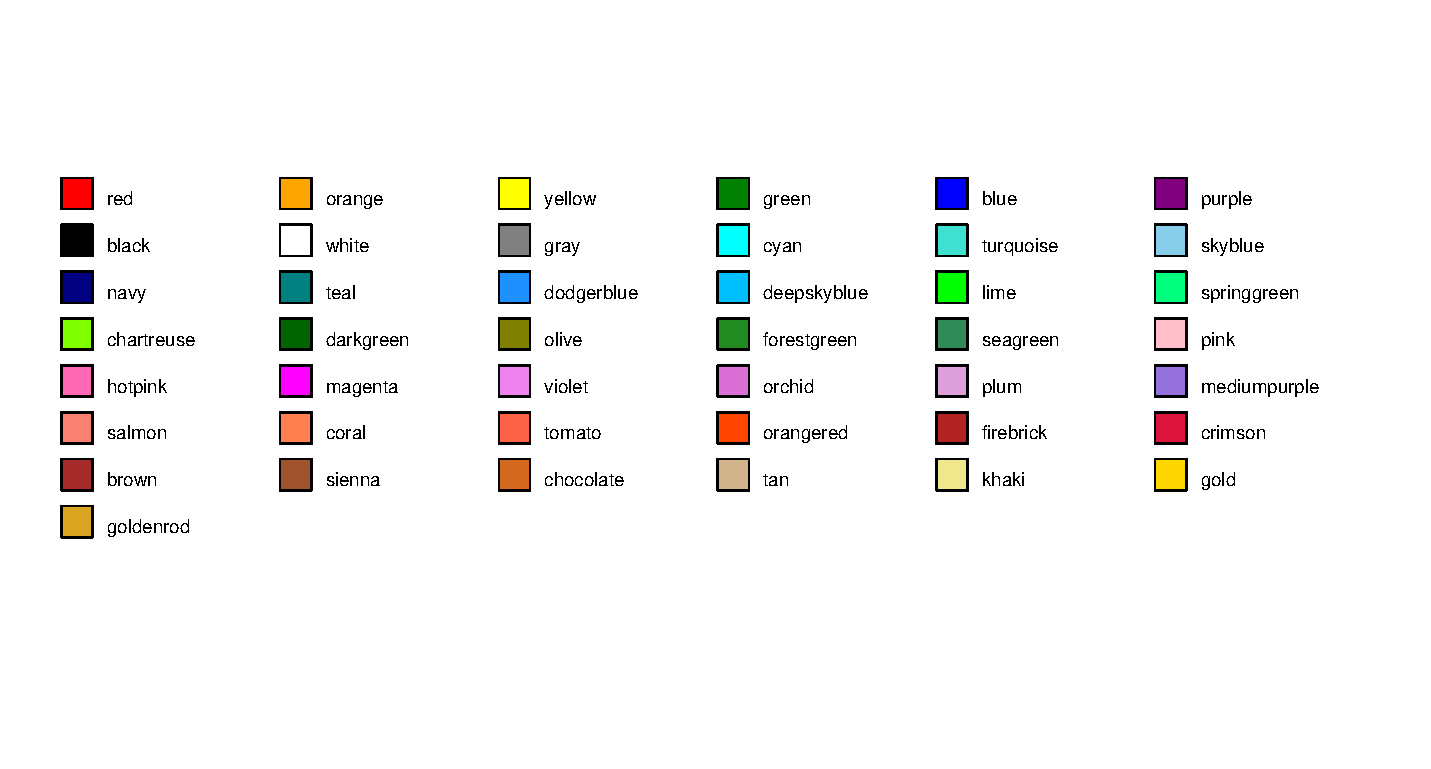
\includegraphics[width=\linewidth, trim={0 3cm 0 3cm}]{../week2/figures/turtle-colors.eps}
  \caption{Some common Turtle colors that you can use. Get creative!}
  \label{fig:turtlecolors}
\end{figure}

\section{Re-using models}

One of the benefits of saving our rules is that we can do the same thing over again. Above, we
created a precise description of a square. Now we need to figure out a way to re-use it.

The first way to re-use rules is to save them into a \term{file}. We call rules that we save on a
computer \term{source code}.

Let's try saving a rule. Open up Thonny and, instead of the prompt, point your mouse at the editor
(\prettyref{fig:thonny-interface}). Rules that we type here can be saved on the computer.
\hint{You can also access all these files on the internet at \url{\giturl}.\\
\begin{center}
\qrcode{\giturl}
\end{center}
}

\hint{Ask your teacher to help you find the \texttt{csforkids} code folder.}
\begin{marginfigure}
  \centering
  \includegraphics[width=0.8\textwidth]{../week2/figures/thonny-run.png}
  \caption{The ``Run'' button at the top of the Thonny interface lets you run code saved in a file.}
  \label{fig:thonny-run}
\end{marginfigure}
\begin{TryThisBox}
  Type the following into the editor and then save it in a file named
  \texttt{duck.py} inside the top-level \texttt{csforkids} folder.

  You can load this file by clicking the green ``Run'' button in the Thonny interface as shown in \prettyref{fig:thonny-run}.
  \begin{lstlisting}
from week2.draw import *<ENTER>
<ENTER>
draw(<ENTER>
  color('blue') +<ENTER>
  forward(100) + turn('right') +<ENTER>
  forward(100) + turn('right') +<ENTER>
  forward(100) + turn('right') +<ENTER>
  forward(100)<ENTER>
)<ENTER>
  \end{lstlisting}
  \tcblower
  You should get something like this:\\
  \includegraphics[width=0.7\linewidth, trim={0 2cm 0 2cm}]{../week2/figures/onesquare.eps}
\end{TryThisBox}

\subsection{Introducing \kw{def}}

That's good, but computers can draw squares without loading
files. This is where the \kw{def} rule come in. Here's how it works.

When we have a bunch of rules we want to re-use, we can use \kw{def} to give a \emph{name} to our
rules. Then, underneath
\kw{def}, we write the rules that make up the new rule. The rules underneath have to be \term{indented}, which means that we have to type two
{\spacekey}s before typing the rule.\curious{Python is known as an \emph{indentation-aware}
language. Some languages do not care about spaces and have other ways to figure out which rules
belong as sub-rules of other rules. But for now, we'll stick with how Python does things!}

\begin{TryThisBox}
  Type the following into \texttt{duck.py}:
  \begin{lstlisting}
def square():
  draw(<ENTER>
    color('blue') +<ENTER>
    forward(100) + turn('right') +<ENTER>
    forward(100) + turn('right') +<ENTER>
    forward(100) + turn('right') +<ENTER>
    forward(100)
  \end{lstlisting}
\end{TryThisBox}

Now try this in the prompt.\hint{Remember to re-run the file (see \prettyref{fig:thonny-run}).}

\begin{replbox}
>>> square()<ENTER>
\end{replbox}

Can we draw two squares? Let's try it?

\begin{replbox}
>>> square()<ENTER>
>>> square()<ENTER>
\end{replbox}

Uh-oh! The second \code{square()} started from a blank screen. This is
because the \code{draw()} rule always starts from a blank
screen. Because we put \code{draw} in our \code{square} rule
above, \code{square} became an action, even though we just wanted the
\emph{data} that was describing our drawing.

Let's be clear about what happened.

\begin{enumerate}
\item You used the \code{square()} rule.
\item Inside \code{square()}, \code{draw()} drew the drawing we gave to it, which is one square on a new blank screen.
\item You used the \code{square()} rule \emph{again}.
\item This caused \code{draw()} to do what it \emph{always} does, which is to create a blank screen and draw a square.
\end{enumerate}

If we want to draw two squares, we're going to have to combine the
rules that just specified the \emph{data} that describes the
square. Let's try it.

\hint{The \code{\textbackslash} at the end of the line means to treat the next line as part of the
  current line. You can skip them if you want and write everything on one line, but such long lines
  won't fit on this page!}
\begin{TryThisBox}
  Type the following into \texttt{duck.py} \begin{lstlisting}
def square_shape():
  color('blue') + \<ENTER>
  forward(100) + turn('right') + \<ENTER>
  forward(100) + turn('right') + \<ENTER>
  forward(100) + turn('right') + \<ENTER>
  forward(100)
  \end{lstlisting}
\end{TryThisBox}

Reload the file by hitting the ``Run'' button and let's try it.

\begin{replbox}
>>> draw(square_shape() + forward(200) + square_shape())<ENTER>
\end{replbox}

Uh-oh! That didn't work. What's going on?

Remember above how the \code{forward()} was a \emph{plan} for a
drawing, but not the drawing itself? We were able to see the plan, by
just using \code{forward()} without \code{draw()}. Let's see
if we can figure out what's going on with \code{square\_shape()}.

First, let's think about what we want. We would want
\code{square\_shape()} to be a drawing plan that went forward four
times, and turned right each time.

Is that what really happens?

\hint{Even though \code{square\_shape()} didn't do what we wanted,
  Python never gave an error. That's because \code{square\_shape()} is
  not an error according to Python. Python just followed its rules
  exactly -- they just weren't the same as the rules we had in mind.}
\begin{replbox}
>>> square_shape()
\end{replbox}

Nothing comes out!

\subsection{The \kw{return} rule}

Here's what's going on. Inside \code{square\_shape()}, we wrote down a
drawing plan, but we never told Python what to do with that plan. In
the prompt, rules that make data cause Python to respond with that
data. Inside a \kw{def}, Python just throws it away, because we didn't
ask Python to keep it.

We use the word \kw{return} inside \kw{def} to say: I've made some data, and this is what I want to
keep. This is the word we need to get Python to keep our plan. Go ahead and modify
\code{square\_shape()}.

\hint{Make sure to pay attention to indentation. You have to add
  spaces in front of \code{forward} in order to keep it ``under''
  the \kw{return}. You can also choose to type it all on one
  line. Remember \code{\textbackslash} is just a convenience.}
\begin{TryThisBox}
\begin{lstlisting}
def square_shape():
  @@return@@ color('blue') + \<ENTER>
    forward(100) + turn('right') + \<ENTER>
    forward(100) + turn('right') + \<ENTER>
    forward(100) + turn('right') + \<ENTER>
    forward(100)
\end{lstlisting}
\end{TryThisBox}

Now, let's see if it does what we expect:

% TODO
\begin{replbox}
>>> square_shape()
\end{replbox}

\begin{BigIdeaBox}
  We can enter as many rules as we want into \kw{def} but we have
  to use \kw{return} if we want Python to respond with particular data.
\end{BigIdeaBox}

\subsection{Combining rules}

Now \code{square\_shape()} results in the drawing plan for a square. Programmers often say that
\code{square\_shape()} \term{evaluates} into the drawing plan for a square, and this is the
terminology we'll use from now on.

We can now use \code{square\_shape()}  with \code{draw()}.

\begin{replbox}
>>> draw(square_shape() + forward(200) + square_shape())
\end{replbox}

And there's two squares!

\begin{bookbox}
\begin{DeepDiveBox}
  \boxtitle{Angles and \code{draw.turn}}
  \label{deepdive:draw-turn-angles}

  \tikzmarknode{angle names}{}
  \code{draw.turn()} \emph{turns} the Turtle cursor. Remember that the cursor is always pointing in
  a particular direction. Turning doesn't cause anything to be drawn, but it does cause future
  \code{draw.forward}s (and other rules) to start off in that direction.

  Angles are measured in \term{degrees}. If you turn 180 degrees (also written as $180^{\circ}$) then
  you turn to face the opposite direction. If you turn 360 degrees (twice 180), then you end up
  facing the same way. By convention, Turtle always turns counter-clockwise, so turning 90 degrees
  (one-half 180) means you end up turning left.

  What if you want to turn right? Remember, you can always turn 180 degrees to turn the other
  direction. From there, turning 90 degrees to the left would leave you facing rightwards of your
  original position. Thus, to turn right, you need to turn 270 degrees. The diagram below shows some
  common angles you might need to know.

  \begin{center}
    \begin{tikzpicture}
      \draw[<->] (0, -2) -- (0, 2) node[above, xshift=1em] {$y$};
      \draw[<->] (-2, 0) -- (2, 0) node[anchor=west, yshift=-0.5em] {$x$};
      \draw[->, green, thick] (0.5,0) arc (0:90:0.5) node[midway,xshift=0.5em,yshift=0.5em] {$90^{\circ}$};
      \draw[->, blue, thick] (1,0) arc (0:180:1) node[pos=0.7,anchor=south east] {$180^{\circ}$};
      \draw[->, orange, thick] (1.5,0) arc (0:270:1.5) node[pos=0.8,anchor=north east] {$270^{\circ}$};
      \draw[->, red, thick] (2,0) arc (0:360:2) node[pos=0.8,anchor=north west] {$360^{\circ}$};
    \end{tikzpicture}
  \end{center}
\end{DeepDiveBox}
\end{bookbox}
\onfloatpage{deepdive:draw-turn-angles}{
  \makemargmark{angle names}{
    \code{draw.turn()} allows the following angle names as shortcuts:
    \begin{description}
    \item[\kw{'right'}] Turn towards the right
    \item[\kw{'left'}] Turn towards the left
    \item[\kw{'around'}] Turn all the way around so you're facing the opposite direction
    \end{description}
  }
}

\subsection{Complex Rules}

\begin{table*}[t]
  \fixfigure
  \begin{tabular}{p{0.24\linewidth}p{0.76\linewidth}}
    \toprule
    Rule & What it does\\\midrule
    \code{draw.goto(x, y)} & Move the pen to the particular \code{x} and \code{y} coordinate.\\
    \code{draw.forward(x)} & Move forward \code{x} units in the current direction of the pen.\\
    \code{draw.circle(r)} & Draw a complete circle with the given radius \code{r}. \\
    \code{draw.circle(r, p)} & Draw a portion of a circle with radius \code{r}. The \code{p} argument specifies what percent of the circle to draw. For example, \code{p} of 0.5 draws a half-circle. \\
    \code{draw.penup()} & Lift the pen \emph{up}. Future movement commands will not draw anything.\\
    \code{draw.pendown()} & Place the pen back \emph{down}. Future movement commands will draw.\\
    \code{draw.color(c)} & Change the color of the pen.\\
    \code{draw.pensize(s)} & Change the size of the tip of the pen.\\
    \code{draw.fill(c, pic)} & Draw \code{pic} and fill in all enclosed areas with color \code{c}.\\
    \code{draw.turn(angle)} & Turn by the given angle, which can be an angle (in degrees), or \code{``left''} or \code{``right''}. \\
    \code{draw.wait(s)} & Wait \code{s} seconds before proceeding. Let's you see how the drawing progresses. \\
    \code{draw.pause(prompt)} & Pause the drawing and display the word \code{prompt} until the user hits \enterkey \\
    \bottomrule
  \end{tabular}
  \caption[][1ex]{These are all the Turtle rules you can use and combine
    together using functions!}
  \label{tab:turtle}
\end{table*}

Grouping rules in this way is a fundamental part of computer programming. Computer programmers have
special names for rules built using \kw{def} and \kw{return}. We call them
\term{functions}. Functions allow complicated things, like shapes, to be hidden away inside rules
that are easier to understand. Now that you've made a \code{square\_shape()}, you can forget all the
details involved with drawing a square. Whenever you need a square, you can just use
\code{square\_shape()}!

\begin{replbox}
draw.draw(
  draw.color('blue') + square_shape() +
  draw.color('red') + square_shape())<ENTER>
\end{replbox}
% TODO GRAPHICS\includegraphics[width=0.8\linewidth]{../week2/figures/twosquares1.eps}

We did that without ever worrying about exactly \emph{how} the square was drawn.\curious{Much of Python itself is written using \kw{def} and \kw{return}. The rules we make with them are no less real than the rules that come with Python.}

\subsection{Arguments}

One of the limitations of \code{square\_shape()} is that it only draws squares of one size. If we
wanted to draw a square for the duck's body and then a smaller square for the duck's head, then we
would have to write two functions that looked the same, like below:

\begin{TryThisBox}
\begin{lstlisting}
def big_square_shape():
  return color('blue') + \<ENTER>
    forward(200) + turn('right') + \<ENTER>
    forward(200) + turn('right') + \<ENTER>
    forward(200) + turn('right') + \<ENTER>
    forward(200)

def small_square_shape():
  return color('blue') + \<ENTER>
    forward(100) + turn('right') + \<ENTER>
    forward(100) + turn('right') + \<ENTER>
    forward(100) + turn('right') + \<ENTER>
    forward(100)
\end{lstlisting}
\end{TryThisBox}

This would quickly get unwieldy. We used \kw{return} to get data out of our function. Now we need a
way to put data \emph{in}. This is what \term{arguments} are.

Arguments are placeholders for things that we don't know yet. Here's a function that could draw a
square of any size:

\begin{TryThisBox}
\begin{lstlisting}
def square_shape(n):
  return color('blue') + \<ENTER>
    forward(n) + turn('right') + \<ENTER>
    forward(n) + turn('right') + \<ENTER>
    forward(n) + turn('right') + \<ENTER>
    forward(n)
\end{lstlisting}
\end{TryThisBox}

Let's see how to use it:

\mTrackBox{Graphics}{ The sort of drawing we are doing with Turtle is called \term{vector
    graphics}. Vector graphics store details on shapes and colors. Because computers can draw shapes
  at any size, vector graphics can be scaled to any size. Your square could be bigger than your
  classroom!}
\begin{replboxannotated}
>>> draw.draw(
...   draw.color('blue') + square\_shape(100) +
...   draw.color('red') + square\_shape(200))<ENTER>
\tcblower
\includegraphics[trim={0 0 0 3cm}, width=0.8\linewidth]{../week2/figures/twosquares1.eps}
\end{replboxannotated}

There's one problem: all of these programs draw the second square in a different way than the first. The
second square appears on top of the first square, instead of in the same position. What's going on?

\section{Errors with Data}

When we originally wrote \code{square\_shape()}, Python did not make a fuss. However
\code{square\_shape()} did not work the way we expected it to. When our expectation of how things
work does not match what actually happens, we call it a \term{bug}.\didyouknow{The first computers
  stored data using vacuum tubes, which were like lightbulbs that could either be switched on or
  off. Vacuum tubes were large and unwieldy and not as reliable as the computers we use today. The
  warm and bright tubes attracted insects, and these insects would sometimes cause the tubes to
  short-circuit. This is the origin of the word \term{bug}! Yuck!}

The squares appearing atop each other instead of in the same spot is another example of a bug.

We work through errors in a process called \term{debugging}. One of the ways in which we debug is by
asking the program to \emph{stop} before it's completed so we can see what it's doing.

The Turtle library we are using provides a simple way to stop the drawing so we can look at it.

\begin{replbox}
>>> draw.draw(draw.pause('square 1') +<ENTER>
... draw.color('blue') + square_shape(200) +<ENTER>
... draw.pause('square 2') + draw.color('red') +<ENTER>
... square_shape(200)
\end{replbox}

\hint{You can always get back to
  the prompt and quit what you're currently doing by holding down both \controlkey and
  \litkey{C}. This is known as an \emph{interrupt}.}
The \code{draw.pause} rule causes Python to \emph{pause} before each square is drawn and wait for
you to type \enterkey in the prompt before it continues drawing.

You should get something like \prettyref{fig:twosquares-debug}.

\begin{figure}
  \fixfigure
  \label{fig:twosquares-debug}
  \centering
  \begin{minipage}{0.48\linewidth}
    \centering
    \includegraphics[width=\linewidth, trim={0 0 0 4cm}]{../week2/figures/twosquares-debug-square 1.eps}\\
    The First Square
  \end{minipage}
  \hfill
  \begin{minipage}{0.48\linewidth}
    \centering
    \includegraphics[width=\linewidth, trim={0 0 0 4cm}]{../week2/figures/twosquares-debug-square 2.eps}\\
    The Second Square
  \end{minipage}
  \caption{What it looks like before each square is drawn. Can you
    spot the difference?

    \textbf{Hint:} Look at the arrow.}
\end{figure}

What do you notice about the arrow in each picture? In Turtle, this arrow is called the
\emph{cursor} and its direction changes how \code{draw.forward} works. If the arrow is pointing
right, then \code{draw.forward} draws to the right. Similarly, if the arrow is pointing towards the
top, then \code{draw.forward} draws towards the top. If you look at the arrow, you'll notice that,
before the first square, it points right, and before the second, it points upward.

How do we fix this issue? The cursor starts pointing right by default. It points upward after the
first square is drawn using the \code{square} function. How do we get it to point right again? Can
you think of an answer?

\begin{BigIdeaBox}
  Sometimes, when combining programs together, things don't work the
  way we expect because our mental model of how the computer ought to
  have done something doesn't match the exact set of rules the
  computer followed.

  It often helps to use tools like \code{draw.pause} to inspect what
  is happening in the middle of our program.
\end{BigIdeaBox}

Here's the solution (pay attention to the italicized part!)

\begin{TryThisBox}
  \begin{lstlisting}
def square_shape(n):
  return \
    draw.forward(n) + draw.turn('right') + \
    draw.forward(n) + draw.turn('right') + \
    draw.forward(n) + draw.turn('right') + \
    draw.forward(n)@@ + draw.turn('right')@@
  \end{lstlisting}
\end{TryThisBox}

Now, our squares are drawn the same way, but they overlap, just like we expected.

\includegraphics[width=0.8\textwidth, trim={0 0 0 4cm}]{../week2/figures/twosquares-fixed.eps}

\subsection{Going Full Circle}

Squares and lines are interesting, but it would be hard to do a lot of
interesting drawing using just those. Let's look at some other shapes.

The first shape we'll introduce is a \emph{circle}. A circle is defined by its radius, which is half
the total distance across the circle. For example, to draw a circle with a 30 unit radius, we can
use \code{draw.circle(30)}. Try this and see what happens.

\begin{replbox}
  draw.draw(draw.circle(30))
\end{replbox}

But there's more, you can also draw \emph{parts} of a circle. This is
called an \emph{arc}. To draw an arc, you can use
\code{draw.circle(30, 1/2)}, which will only draw \emph{half} the
circle\hint{You can use \code{1/2} or \code{0.5}. Python understands
  both.}

\begin{replbox}
draw.draw(draw.circle(30, 0.5))<ENTER>
draw.draw(draw.circle(40, 1))<ENTER>
draw.draw(draw.circle(20, 1/3))<ENTER>
\end{replbox}

Now, try drawing this figure.

\includegraphics[width=0.5\textwidth,trim={0 3cm 0 0}]{../week2/figures/lrcircle.eps}

Having trouble? Think back to the examples we tried above. Which way
did the arrow move when drawing the circle?

Turtle assumes that when we want a circle, we always want to draw it in this direction
(counter-clockwise). To make it draw in a clockwise direction, we supply it a \emph{negative} radius
(see \prettyref{fig:turtle-circles}). This arrangement where a computer system always does things
one way and requires the programmer to explicitly choose another way is called a \term{default}.

\begin{figure}[p]
  \fixfigure
  \label{fig:turtle-circles}
  \caption{The \code{draw.circle} rule produces some portion of a circle with a particular radius,
    as illustrated above. A positive radius corresponds to a point to the ``left'' of the cursors
    direction. A negative radius means to go to the right.

    The diagram here demonstrates the result of

    \code{draw.circle(30, 0.15) + draw.circle(-15,0.6)}
  }
  \begin{tikzpicture}[font={\sffamily\footnotesize}]
    \pgfmathsetmacro{\angleone}{2 * pi/360 * -100}
    \pgfmathsetmacro{\circleportion}{0.15}
    \pgfmathsetmacro{\circleportiontwo}{0.6}
    \pgfmathsetmacro{\circleportiontworad}{\circleportiontwo * 2 * pi}
    \pgfmathsetmacro{\circleportionrad}{\circleportion * 2 * pi}

    \pgfmathsetmacro{\circleonefinalangle}{\angleone+\circleportionrad}
    \pgfmathsetmacro{\midx}{cos(\circleonefinalangle r) * 2}
    \pgfmathsetmacro{\midy}{sin(\circleonefinalangle r) * 2}
    \pgfmathsetmacro{\circletwox}{cos(\circleonefinalangle r) * 3}
    \pgfmathsetmacro{\circletwoy}{sin(\circleonefinalangle r) * 3}
    \pgfmathsetmacro{\circletwostart}{acos(\midx - \circletwox)}
    \pgfmathsetmacro{\finalx}{\circletwox + cos((\circletwostart + \circleportiontworad) r)}
    \pgfmathsetmacro{\finaly}{\circletwoy + sin((\circletwostart + \circleportiontworad) r)}

    \draw[magenta, thick, dashed] (0,0) circle (2);
    \draw[violet, thick, dashed] (\circletwox,\circletwoy) circle(1);

    \draw[->,dashed,color=IdeaBlue] ({cos(\angleone r) * 2}, {sin(\angleone r) * 2}) -- (0, 0);
    \draw[->,dashed,color=IdeaBlue] (\finalx, \finaly) -- (\circletwox, \circletwoy);

    \draw[decorate, decoration={brace, amplitude=5pt, mirror, raise=0.2em}] (0,0) -- ({cos(\angleone r) * 1.9}, {sin(\angleone r) * 1.9}) node[midway, xshift=-2.1em] {$r = 30$};
    \draw[decorate, decoration={brace, amplitude=5pt, raise=0.3em}] ({\finalx * 0.98}, {\finaly * 0.98}) -- (\circletwox, \circletwoy) node[midway, xshift=-1.5em, yshift=-1.5em] {$r = -15$};

    \draw[black, ultra thick, {Stealth[reversed]}-{Stealth}] ({cos(\angleone r) * 2}, {sin(\angleone r) * 2}) arc ({deg(\angleone)}:{deg(\circleportionrad + \angleone)}:2) node[midway,name=arc] {};
    \draw[black, ultra thick, {Stealth-}] (\finalx,\finaly) arc
                                                    ({deg(\circletwostart+\circleportiontworad)}:{deg(2 * pi + \circletwostart) + 13}:1) node[midway,name=arctwo]{};
    \draw[dashed,xshift=0.3em,yshift=-0.3em, <-] (arc) to [bend left] ++(-2em, -4em) node[below] {\texttt{draw.circle(30, \circleportion)}};
    \draw[dashed,xshift=0.3em,yshift=0.3em, <-] (arctwo) to [bend right] ++(4em,2em) node[above] {\texttt{draw.circle(-15, \circleportiontwo)}};

\end{tikzpicture}

\end{figure}

To draw the diagram, use this code:
\curious{Try using \code{draw.pause} to visualize exactly which
  portion is drawn by which command!}
\tikzforeground{
  \coordinate (immediate note middle) at ($(immediate note target)!0.5!(immediate note target end)$);
  \node[anchor=west] (immediate note hint) at ([xshift=0.7cm,yshift=-0.2cm]current page text area.east|-immediate note middle) {
    \begin{tcolorbox}[code note]
      You can set \code{immediate=True} to just get the final output, without having to watch Turtle draw.
    \end{tcolorbox}
  };

  \draw[->] (immediate note hint.west) to[out=180,in=-40,looseness=0.8] ($(immediate note target)!0.8!(immediate note target end)$);
}
\begin{replbox}
>>> draw.draw(draw.circle(30, 1/2) + draw.circle(-30, 1/2), (*@\tikzmarknode{immediate note target}{}@*)immediate=True(*@\tikzmarknode{immediate note target end}{}@*))
\end{replbox}

With these shapes, we can make more complicated figures. There's just
one thing left: filling our shapes with color.

We saw how to change the color of the lines we drew, but how do we
\emph{fill} the shapes we draw with a color?

The \code{draw} module provides the \code{draw.fill} rule to create
filled diagrams. Let's try it.

\begin{replbox}
>>> draw.draw(draw.fill('blue', square_shape(100)))<ENTER>
\end{replbox}

\section{The Duck Challenge}

\hint{Start by getting the basic shapes. Then change lengths and measures until it's just right. Try it!}
Remember how we started class by drawing a duck and attempting to describe it to our friend? At that
point we lacked a proper language to talk about drawings. But now we have a way to talk about
drawings precisely! Take a look at your drawing, and break it up into \emph{rules}: lines, circles, etc.
\didyouknow{One of the earliest kinds of computers was known as the
  \textbf{Jacquard Loom}. It revolutionized the manufacture of complex
  patterns in cloth. Weavers would punch cards giving the machine
  directions to raise or lower threads to create complex patterns.

  \begin{center}
    \includegraphics[width=0.9\linewidth]{../week2/figures/Jacquard.loom.cards.jpg}
  \end{center}
}
\begin{TryThisBox}
  Try using what you've learned thus far to draw a duck using \kw{def} and \kw{return} and
  Turtle. Name your function \code{duck}.

  As you're doing this, try to keep re-usable parts of your duck in separate functions, so you don't
  have to figure out the same code over and over again
\end{TryThisBox}

Here are some examples of what you may have created. All of these are examples of a ``duck'' that
you can make using the simple rules for drawing we learned above.

\begin{BigIdeaBox}
  To the computer, there is no duck. It's just a set of rules you told it to follow to draw one
  depiction of a duck that you found useful. We have tonundeesrand the problems we are trying to solve precisely to program them into a conputer.
\end{BigIdeaBox}

\section{Copying Ducks}

You've now drawn \emph{one} duck; what if we wanted more? The whole point of this was to codify
exactly how to make a duck and explain that precisely. Now, with these instructions in hand,
we can make more ducks.

\begin{replbox}
>>> from week2.examples import *<ENTER>
>>> lake_of(duck)<ENTER>
\end{replbox}

Nice! Look at all those ducks. But, there's one problem... all our ducks look the same. Can we make
each one a bit more unique?
\mTrackBox{Music \& Sound}{ We've seen how computers represent images as
  lights going on and off, but how do they represent \emph{sound}?

  When our ears hear sound, they are responding to \emph{changes} in
  air pressure.

  Computers represent this -- you guessed it -- using numbers!

  With graphics, we had to break up the rectangular screen into small
  chunks called pixels. For sound, we instead break up \emph{time}
  into really small sections (tens of thousands per second!) called
  samples. Within each sample, we store a number which represents how strong the sound is at that time. The samples
  are sequenced together rapidly using a componenty called a DAC or
  \term{digital-to-analog converter} and sent to a speaker, which outputs a very short sound at that strength. This process happens tens of thousands of times in one second. Our ear perceives it as high quality sound. }


Let's add some \term{arguments} to our \code{duck} function. Modify
your function to include some arguments.  \hint{The \code{lake_of}
  function supports \code{body_color}, \code{eye_color}, and
  \code{size}, and will use whatever arguments your function has. The
  colors can be used however you want, and the size just says how
  ``big'' to draw the duck. Try it and see!}
\begin{TryThisBox}
  \begin{lstlisting}
def duck(@@body_color@@, @@eye_color@@):
  @@your code@@
  \end{lstlisting}
\end{TryThisBox}

Now, take these arguments and use it to change your duck's body and eye color using the
\code{draw.color} and \code{draw.fill} functions we saw above.

Now, rerun the example above:

\begin{replbox}
from week2.examples import *<ENTER>
lake_of(duck)
\end{replbox}

Much better!

\begin{BigIdeaBox}
  Since we packaged our duck into a function and added arguments to allow certain parts to change,
  we made it trivial to re-use our duck many times. This is a foundational part of computer
  programming.
\end{BigIdeaBox}

\section{Conclusion: From Drawing to Computation}

In this lesson we learned that we can often do things by hand that
take effort to describe to the computer. This is because computers are
precise and follow fixed rules. Once we are able to describe things
precisely, then we can describe them to a computer and manipulate
them. Python lets us store descriptions in \term{source code} or in
\term{functions} which we write using \kw{def} and \kw{return}.

Everything in computer science is a description of something real
(whether a physical item or a real problem) that we want to solve. To
be able to manipulate things with computers we have to be able to
express our problem as rules the computer understands. In the case of
visual information, it means understanding graphics like the Turtle
system. Even though the computers don't \emph{understand} what a duck
is, we were able to describe a drawing of a duck to the computer. In
the next chapters, we'll explore other ways of describing the world to
a computer.

\Exercises

\begin{exercises}
\item Try creating some other animal as a Python function, and using
  it with the \code{lake\_of} function we used before. What does this
  show about Python's \emph{understanding} of the thing we drew?
  \answer{Whichever animal we draw, Python and the lake\_of
    function treat it the same way. Each animal is just a rule
    for Python to draw.}

\item A \emph{regular} polygon is a shape with some number of sides whose sides are all of equal
  lengths. Can you think of a way to write a function that represent a drawing of a regular polygon
  of any number of sides? For example, an equilateral triangle (see below) is the simplest
  polygon. It has three sides, all of the same length. How would you draw this in Turtle? What about
  a square? A pentagon? A hexagon?

  \hintnote The sum of all angles in any polygon sum to $180(n - 2)$, where $n$ is the number of
  sides. So the angles of a triangle always sum to $180(3 - 2) = 180$ degrees.

  \begin{center}
  \begin{tikzpicture}
    \coordinate[label=left:$A$]  (A) at (0,0);
    \coordinate[label=right:$B$] (B) at (4,0);
    \coordinate[label=above:$C$] (C) at (2,3.464);

    \coordinate[label=below:$c$](c) at ($ (A)!.5!(B) $);
    \coordinate[label=left:$b$] (b) at ($ (A)!.5!(C) $);
    \coordinate[label=right:$a$](a) at ($ (B)!.5!(C) $);

    % angle alpha
    \draw[fill=green!30] (0,0) -- (0:0.75cm) arc (0:60:.75cm);
    \draw (0.36cm,0.25cm) node {\small $60^{\circ}$};

    % angle beta
    \begin{scope}[shift={(4cm,0cm)}]
      \draw[fill=green!30] (0,0) -- (-180:0.75cm) arc (180:120:0.75cm);
      \draw (150:0.5cm) node {\small $60^{\circ}$};
    \end{scope}

    % angle gamma
    \begin{scope}[shift={(60:4)}]
      \draw[fill=green!30] (0,0) -- (-120:.75cm) arc (-120:-60:.75cm);
      \draw (-90:0.5cm) node {\small $60^{\circ}$};
    \end{scope}

    % the triangle
    \draw [line width=1.5pt] (A) -- (B) -- (C) -- cycle;
  \end{tikzpicture}
  \end{center}
\item An animation is a series of still images. The \code{lake\_of} function uses your duck function
  to create a simple animation of ducks swimming in a lake. You can do the same thing using
  \code{draw.draw()} function with \code{immediate=True} and the \code{draw.wait} function. Try it!
\end{exercises}

% Show red and blue yin/yan thing
% # ============================================================
% # Chapter 2 TODO Outline (Technical-first)
% # ============================================================
% 
% * Drawing Primitives (Missing Technical Core) - Done
% - Introduce arcs / circles as drawing primitives - Done
% - Show how arcs differ from straight lines - Done
% - Explain radius + angle intuitively (no formulas yet) - Need to ADD diagram
% - Add example: combining lines + arcs -- NOT DONE
% - Add figure showing arc parameters visually -- TODO
% 
% * Filling and Regions -- DONE
% - Introduce closed shapes -- TODO
% - Explain what ?inside? vs ?outside? means -- TODO
% - Introduce fill as coloring a region - DONE
% - Show same outline with and without fill - Add diagram TODO
% 
% * Multiple Duck Representations (Technical)
%     - Draw duck using only lines
%     - Draw duck using lines + arcs
%     - Draw duck using fill
% - Compare versions side-by-side
% - Ask: what details were added / removed?
% 
% * Modeling Choices -- will not do
% - Explicitly name ?model? at this point
% - Identify what each duck drawing ignores -- figure caption
% - Identify what each drawing keeps -- figure caption
% - Add diagram: same duck, different models
% 
% * Simulation: A Lake of Ducks
% - Introduce idea of many ducks, same rules -- done
% - Add simple rule-based placement (position, size, direction)
% - Show variation via parameters -- done
% - Simulate multiple ducks on a lake
% - Add figure: single duck vs many ducks
% 
% * Abstraction via Parameters -- colors of body, and eyes
% - Name parameters explicitly -- 
% - Show how changing numbers canges appearance -- TODO
% - Connect parameters to ?knobvs? on the model -- no
% 
% * From Drawing to Computation
% - State: computer draws by following rules
% - Emphasize repeatability
% - Emphasize no understanding of ?duck?
% 
% * Curiosity / Track Boxes (Insert Where Natural)
% - Graphics: circles aren?t really circles
% - Games: fake physics
% - Sound: sound as numbers
% - Simulation: same rules, many agents
% 
% * Conceptual Wrap-Up
% - Revisit duck question one last time
% - State: model ? thing
% - State: computers work only with models
% - End with forward-looking question
% 
% # ============================================================

% -*- mode: latex -*-

\week[description={Last week we discussed information. This week we start to understand that combining information with decision making is the foundation on which we can build complex behaviors.}]{Making Decisions}

\resource[silent,files={motherduck.html},description={Play the DuckBot game online},text={DuckBot}]{demos/duckbot.html}
\resourcegen{name=data/duckbot.tar.gz, type={archive}, from={week3 game.py sample_brain.py assets/tileset.json assets/maps/level1.json assets/maps/level2.json assets/maps/level3.json assets/duck.png assets/terrain_atlas.png}}
\resourcegen{name=demos/duckbot.html, from=week3/site/duckbot.html, type={jinja}}

The ancient Greek polymath Eratosthenes regularly traveled between the Egyptian cities of Syene and
Alexandria (see \prettyref{fig:alexandria}). He was a very observant scientist, and -- like many
ancient polymaths -- was interested in astronomy. He noticed that, on the summer solstice, the
following things were true (see \prettyref{fig:eratosthenes}):
\begin{marginfigure}
  \centering
  \includegraphics[width=0.9\marginparwidth]{../week3/figures/syene-alexandria.jpg}

  \caption{The distance between the Egyptian cities of Alexandria and Syene is 5000 stadia or approximately 787.5 kilometers apart.}
  \label{fig:alexandria}
\end{marginfigure}

\begin{enumerate}
\item In Syene, which was south of Alexandria, on the summer solstice, the sun shone straight down. If he looked at the bottom of a deep well, there were no shadows at all. If you planted a stick in the ground, the stick would cast no shadow, because the sun was directly overhead.
\item In Alexandria, to the north, on the same day at the same time, if you planted a stick in the ground, there was a shadow.
\end{enumerate}

What can be deduced based off these two observations?

Here's some more details: the straight-line distance between the two cities is approximately 787.5
kilometers apart. Also, the angle of the shadow cast on the ground in Alexandria was $7.5^{\circ}$.

Eratosthenes did the following calculation:

\[
\underbrace{787.5\;\text{kilometers}}_{\text{distance between the two cities}} \times \frac{360^{\circ}}{7.5^{\circ}} \approx 40,000\;\text{kilometers}
\]

\begin{figure}
  \centering

  \begin{tikzpicture}[scale=0.5,font={\sffamily}]
    \node at (0, 10) {Sun};
    \draw (0, 10) circle (1);
    \draw (-2, 0) -- (10, 0) node[midway, anchor=north, yshift=-0.1em] {Ground};

    \draw (0,0) -- (0, 4);

    \coordinate (alexandria bottom) at (6, 0);
    \coordinate (alexandria stick) at (6, 4);

    \path[name path=ray] (alexandria stick) -- ++(-82.5:100);
    \path[name path=x axis] (-10, 0) -- (10, 0);
    \fill[name intersections={of=ray and x axis, by=B}, dashed, fill=lightgray]
      (alexandria bottom) -- (alexandria stick) -- (B);
    \draw (alexandria bottom) -- (alexandria stick);
    \draw[dashed] (alexandria stick) -- (B);
    \draw[ultra thick] (B) -- (alexandria bottom);

  \end{tikzpicture}

  \caption{Eratosthenes noticed that on the summer solstice the shadows cast by the Sun at noon appeared different in two cities. In Syene, there was no shadow, which meant the Sun was directly overhead. In Alexandria, there was a shadow.}
  \label{fig:eratosthenes}
\end{figure}

\didyouknow{
Albert Einstein famously came up with his theory of special relativity by simply thinking about it!
If you ever study physics in depth, you'll discover that the entirety of special relativity falls
out of two simple facts:
\begin{enumerate}
\item The speed of light is the same for everyone.
\item The relationship between the sides of the triangle: $c^2 = a^2 + b^2$.
\end{enumerate}
Einstein used these simple facts to show that light actually travels less distance in moving
reference frames, leading to one of the most surprising facts about our universe: fast things become
shorter.  }
\begin{BigIdeaBox}
As humans, we only see our part of the world and our part of the universe. The consistent
application of precise rules lets us reason about things larger than what we can directly perceive.

Despite having no possible way to observe the entirety of the planet. Eratosthenes used simple rules
of logic and simple observations to deduce a global truth.
\end{BigIdeaBox}

\section{Week 2 Review}

Last week, we discussed breaking down large drawings and objects into
smaller elements. Doing so let us build large drawings from simple
drawings we could combine together. Even though the set of simple
or \term{primitive} drawings were small, we could draw quite a bit
with them.

\section{Understanding Big Things}

The Turtle cursor we saw last week simply knew what was around it. We
gave it commands based on its \emph{immediate} environment and based
on those, it simply followed what we told it. It was up to us to give
it the set of rules necessary to make the drawings we wanted.

We can use a similar idea to understand large things. It's impossible
to build a system large enough to be able to ``see'' the entire set of
things we'd ever want to talk about. Just like Eratosthenes, we are
limited in what we are able to perceive. Similarly, computers can only
perceive a few things directly, yet we are able to build very complex
systems with them.

How can we use small rules to understand large things? Once again, we have to be clear about our
language. We have to understand what we can see and what we can do with that information. When our
rules are designed to ingest and understand information, we call that
an \term{algorithm}. \didyouknow{The word \emph{algorithm} comes from the name of the Persian
polymath and mathematician al-Khw\={a}rizm\={i} who introduced the idea of algorithms to the West
via his book \emph{kit\={a}b al-\d{h}is\={a}b al-hind\={i}} (``Book of Indian Computation''). This
book was translated into Latin by Robert Chester in 1145, and was the principal mathematics textbook
used in many universities for almost four centuries. Many of our modern methods of addition,
subtraction, division, and multiplication come from his translations!
\vspace{1em}
\begin{center}
  \includegraphics[width=0.6\marginparwidth]{../week3/figures/al-kwharizmi.jpg}
\end{center}}

In order to learn and understand algorithms, we are going to play a simple game. But be
warned... this is not like any game you've played before!

\section{Introducing DuckBot!}

Meet DuckBot! DuckBot has been put in change of a group of three very sneaky little ducklings while
Mother Duck has gone away. But those sneaky little ducklings have fried DuckBot's brain and have run
off. They are now hiding in some corner of the pond. DuckBot needs to find the ducklings before
Mother Duck gets back.

Your job is to give DuckBot a new brain so that it can find the ducklings!

Oh and one more thing: if DuckBot runs into any obstacle, like a rock, a plant, or the ground,
DuckBot dies and will never be able to make it to the ducklings. Your brain has to make sure he only
ever swims in water.

The DuckBot game window (see \prettyref{fig:duckbot}) has four parts:
\begin{enumerate}
\item This shows you where DuckBot is in the pond. You can change your view of the pond by using the
  arrow keys or dragging around with your mouse. You can zoom in or out using the mouse wheel or the
  \litkey{+} and \litkey{-} keys. But remember, whatever you can see doesn't matter, because DuckBot
  can only see what's immediately around it.

\item The brain pane shows you the current Python code in DuckBot's brain. DuckBot runs this code
  each time it moves a square in the pond, in order to decide what to do next. You can edit the code
  here to make DuckBot do what you want.

\item The bottom pane shows you what DuckBot sees. DuckBot can see obstacles in all four cardinal
  directions.

\item The controls pane lets you control DuckBot. You can make DuckBot go or stop by clicking the ``Start Duck'' and ``Stop Duck'' buttons. You can reset the game by clicking the ``Reset Game'' button.\hint{You'll need to stop the duck before resetting the game or reloading DuckBot's brain} When you've made changes to your brain, you have to tell DuckBot to switch to the new brain by clicking the ``Reload Brain'' button.

\end{enumerate}

\subsection{Programming DuckBot}

DuckBot is programmed in Python. The goal of the game is to write a program so that DuckBot swims
over \emph{every} portion of the pond it can reach. The ducklings are \emph{very} sneaky and always
stay in the spot in which DuckBot is least likely to find them. Thus, DuckBot really must visit
every single portion of the pond.

The pond is arranged in a grid. DuckBot moves one square at a time. Once a square on the grid has
been swam over it turns darker, but DuckBot cannot see if it's already swam over a particular
square. It only sees what's around it and responds.

Every time DuckBot moves to a new square, the brain code is run again. The brain decides two things:

\begin{enumerate}

\item The \textbf{direction} that DuckBot ought to go in next.

\item The \textbf{thought} that DuckBot ought to think.

\end{enumerate}

\subsection{The Brain}

DuckBot's brain is written as a function.

% TODO figure showing the function declaration
\begin{minipage}{\textwidth}
  \tikzforeground{
    \node[anchor=south] (brain function note) at ([yshift=2em]brain function name.north) {
      \begin{tcolorbox}[code note, width=2cm]
        Your function should be named \code{brain}.
      \end{tcolorbox}
    };
  }

  \Large \ttfamily
  \begin{tcolorbox}[sharp corners]
    \kw{def} \tikzmarknode{brain function name}{brain}(\tikzmarknode{north arg}{north}, \tikzmarknode{east arg}{east}, \tikzmarknode{south arg}{south}, \tikzmarknode{west arg}{west}, \tikzmarknode{thought arg}{thought}):
  \end{tcolorbox}
\end{minipage}

\termheading{How DuckBot Perceives the World}

DuckBot can sense the four squares immediately to the North, South, East, and West of its current
location.\hint{Remember that Python requires us to surround letters and words in quotation marks.} A
blocked square is signified by the letter \code{'x'}. A free square is signified by the
letter \code{'*'}. This is illustrated in \prettyref{fig:duckbot-directions}.

\termheading{DuckBot's Memory}

As we said before, DuckBot's brain is totally fried and so is its memory. DuckBot can only remember
the last thing you told it. This is called its \emph{thought}.\curious{DuckBot's thought is an
example of \term{state}.} DuckBot can see what's around it in the current square. Based off of this
knowledge \emph{and} its previous thought, DuckBot has to decide the next direction and its next
thought.

You can see DuckBot's current thought in the information pane beneath the pond. When you first start
DuckBot, its thought is the number $0$.

\termheading{Deciding What to do Next}

In order to make DuckBot \emph{do} something, you have to give it instructions. Just like we saw
last week, to send data out of a function we use \kw{return}.

\begin{minipage}{\textwidth}
  \Large \ttfamily
  \tikzforeground{
    \node[anchor=south](return comma note) at ([xshift=1cm,yshift=1em]return comma.north) {
      \begin{tcolorbox}[code note, width=4cm]
        The \code{,} (comma) tells \kw{return} that we are going to send back more than one piece of data.
      \end{tcolorbox}
    };

    \draw[->] (return comma note.south) -- ([yshift=0.1em]return comma.north);
  }
  \begin{tcolorbox}[sharp corners]
    \tikzmarknode{return dir}{\kw{return}} \tikzmarknode{return direction}{'N'}\tikzmarknode{return comma}{,} \tikzmarknode{return next thought}{'next\_thought'}
  \end{tcolorbox}
\end{minipage}

This time, instead of just returning one thing, we're returning two
things. The first thing we return is which direction we want DuckBot
to go in. This can be:

\begin{itemize}
\item \code{'N'} to go north
\item \code{'E'} to go east
\item \code{'S'} to go south
\item \code{'W'} to go west
\item \code{None} to stay in the same place\hint{\code{None} is a
  special Python value indicating the absence of any data. You don't
  need to put it in quotes. If you did, then you would get the string
  \code{'None'} instead of the special \code{None} value}
\end{itemize}

The second thing we return is DuckBot's next thought. The thought can
be anything: a number or a string or even the \code{None}
value.\hint{You'll probably want your thoughts to mostly be
  strings. This will make your code easier to understand.} You get to
decide!

\subsection{Playing the Game}

When you open DuckBot, load a new level or press the ``Reset Game'' button, the pond is cleared and
DuckBot and the ducklings end up in random parts of the pond.\curious{Actually, the ducklings end up
  in the pond you're least likely to end up in. That's why it's so important DuckBot hits the whole
  pond!}

\section{An Example DuckBot Level}

To make things clearer, let's try working through a single DuckBot level. The first level looks like
this:

% TODO duckbot level 1

DuckBot is placed at a random location. DuckBot's brain is the simple function:

\begin{lstlisting}
def brain(north, east, south, west, thought):
  return None, thought
\end{lstlisting}

What will happen if we start DuckBot with this brain? Let's try it. Click the ``Start Duck'' button
in the control pane (see \prettyref{fig:duckbot}). \hint{Remember, always try to \emph{predict} what
  is going to happen before we do anything on the computer.}

Hmm... that's no good. We want DuckBot to do something. Let's make DuckBot go east.

\hint{Remember to click the ``Reload Brain'' button to make DuckBot use the new brain.}
\begin{TryThisBox}
  Change DuckBot's brain to this:
  \begin{lstlisting}
    def brain(north, east, south, west, thought):
      @@return 'E', thought@@
  \end{lstlisting}
\end{TryThisBox}

If you go ahead and run this, DuckBot will head all the way east until it hits the shore. Remember,
DuckBot is very fragile and does exactly what you tell it. If it hits land, it dies, which is what
happens here. We need to detect when there is an obstacle to the east and send DuckBot in a
different direction.

But, in order to do that, we need to figure out how to make our function \kw{return} one thing if
there is something to the east and \kw{return} another thing if not.

\subsection{Using \kw{if}}

\begin{marginfigure}
  \centering
  \includegraphics[width=0.9\marginparwidth]{../week3/figures/grace-hopper.jpg}
  \caption{Rear Admiral Grace Hopper was a famous computer scientist who invented a programming
    language called \term{COBOL} (\textbf{CO}mmon \textbf{B}usiness-\textbf{O}riented
    \textbf{L}anguage) which was one of the first to usewords like \kw{if} to define how programs
    ran. Before her innovation, computer programs were written using difficult machine code and
    obtuse mathematics. For her fundamental contributions to computer science, she was awarded the
    Presidential Medal of Freedom in 2016.}
  \label{fig:grace-hopper}
\end{marginfigure}

Python comes with a special word that does exactly what we want. This is called \kw{if}, and it works like this:

We write \kw{if} followed by a condition, and then a colon. If the condition is true, then the code
beneath the \kw{if} runs. If the condition is false, then all that code is skipped. This is
illustrated in \prettyref{fig:if-statement}.

To understand what it means to be ``beneath'' the \kw{if}, we have to understand how Python treats
the \code{:}. As we learned last week, Python is sensitive to how things are spaced out. When we
write \kw{def}, we have to put spaces to signify which code is part of our function. The same is
true of \kw{if}. \curious{The error thrown is called \code{IndentationError}.}If we want some code
to run when the condition is true, then all this code must be indented \emph{more} than the \kw{if}
statement. Moreover, all the code has to line up. If you indent one line with six spaces, and the
next line with ten, then Python will return an error.

Let's try using \kw{if} to make DuckBot do something if we have an obstacle to the east.

\hint{Note that it has \emph{two} equal signs. The double equal
  signs compares values. A single equal sign has a different meaning, which we'll explore later.}
\begin{TryThisBox}
  Change DuckBot's brain to this:
  \begin{lstlisting}
    def brain(north, east, south, west, thought):
      @@if east == 'x':
        return 'N', thought@@
      return 'E', thought
  \end{lstlisting}
\end{TryThisBox}

Think about what's going to happen now. When you've decided what you think is going to happen to
DuckBot, hit ``Reload Brain'' and start DuckBot.

Uh-oh! DuckBot once again hit an obstacle, but this time it at least turned towards the north, once
it hit an obstacle to the east.

At this point, maybe it's a good idea to check if there's an obstacle to the north. But which
direction to turn then? North was left of east. We could go west, which is left of north.

Of course, if we did that, DuckBot would just go all the way to the west side of the pond, and hit
the wall there. We'll have to handle the west case as well. And then, if we turn south, DuckBot will
hit the bottom of the pond, so we have to turn back east.

\hint{This is one of those changes where it's really important that you try to \emph{predict} what
  is going to happen.}
\begin{TryThisBox}
  Change DuckBot's brain to this:
  \begin{lstlisting}
    def brain(north, east, south, west, thought):
      if east == 'x':
        return 'N', thought
      @@if north == 'x':
        return 'W', thought
      if west == 'x':
        return 'S', thought
      if south == 'x':
        return 'E', thought@@
      return 'E', thought
  \end{lstlisting}
\end{TryThisBox}

If you go ahead and try that, you'll find that poor DuckBot *still* hits the north shore. Clearly
we've not quite figured out how to make this work.

To understand what's going on, let's consider DuckBot at the northeast corner of the pond (see
\prettyref{fig:duckbot-ne}). At this point, \code{north} and \code{east} are \code{'x'} and
\code{south} and \code{west} are \code{'*'}. You can see this at the bottom left of the DuckBot
interface, which displays the current state of what DuckBot sees.

In the brain view, you'll also notice that some lines are highlighted. The lines highlighted in
light gray represent the code that was used by DuckBot to make its decision. The lines highlighted
in green represent points where decisions were made (i.e., places that used \kw{if}). Finaly, the
line highlighted blue indicate where DuckBot made its decision.

If we look at the interface, we'll see that lines 2 and 3 (see \prettyref{listing:duckbot-circle})
are highlighted, indicating that these are what led to the decision DuckBot made. But that's not
what we wanted. We wanted DuckBot to make the decision to turn West, which is on line 5. The \kw{if}
of line 4 was supposed to check the condition that there was an obstacle to the north. But this line
is not highlighted, indicating it was not used. Why?

If you notice, the \kw{if} that checked the obstacle to the east was used, and then, Python saw that
there was an obstacle to the east when DuckBot was in the northeast square. But, this \kw{if} has a
\kw{return} under it. Because the condition in the \kw{if} was true, Python used the code underneath
it, which told the function to immediately send back its decision to go north. This is not what we
wanted. We have to make sure that there's also no obstacle to the north.

\section{Booleans}

In the above code examples, we skipped over how we wrote the \kw{if} conditions, but it's worth
considering them in more detail right now. How does Python know whether a condition is true or not?
This is important to understand when Python is going to run code.

Try this in your Python prompt:

\begin{replbox}
>>> True
True
>>> False
False
\end{replbox}

These values are two special values used by Python to indicate -- as you'd expect -- whether
something is true or false. The collective term for these kinds of values is \term{booleans}.

Booleans can be combined using symbols, similar to addition and multiplication of numbers. For
example, the symbol \kw{and} checks if both sides are \kw{True}, and returns \kw{True} if they
are.

\begin{replbox}
>>> True and False
False
>>> True and True
True
>>> False and False
False
>>> False and True
False
\end{replbox}

The symbol \kw{or} checks if only one side is \kw{True}.

\begin{replbox}
>>> True or False
True
>>> True or True
True
>>> False or False
False
>>> False or True
True
\end{replbox}

There are only two possibilities for the values on each side of a \kw{and} or \kw{or}. Thus, there
are four possible combinations of values that can go into these symbols. We can write out the entire
set of inputs and outputs as a four-row table. These are called \term{truth tables}. The tables for
\kw{and} and \kw{or} are given in \prettyref{fig:and-or-truth-tables}.

\begin{figure}
  \begin{minipage}{0.45\textwidth}
    \begin{center}
      \begin{tabular}{cc|c}
        \multicolumn{3}{c}{\texttt{x}\;\kw{and}\;\texttt{y}} \\\hline
        \texttt{x} & \texttt{y} & \\\hline
        \kw{True} & \kw{True} & \kw{True} \\
        \kw{True} & \kw{False} & \kw{False} \\
        \kw{False} & \kw{True} & \kw{False} \\
        \kw{False} & \kw{False} & \kw{False} \\\hline
      \end{tabular}
    \end{center}
  \end{minipage}
  \begin{minipage}{0.45\textwidth}
    \begin{center}
      \begin{tabular}{cc|c}
        \multicolumn{3}{c}{\texttt{x}\;\kw{or}\;\texttt{y}} \\\hline
        \texttt{x} & \texttt{y} & \\\hline
        \kw{True} & \kw{True} & \kw{True} \\
        \kw{True} & \kw{False} & \kw{True} \\
        \kw{False} & \kw{True} & \kw{True} \\
        \kw{False} & \kw{False} & \kw{False} \\\hline
      \end{tabular}
    \end{center}
  \end{minipage}

  \caption{These are the truth tables for the \kw{and} and \kw{or} rules. The inputs are in the left two columns and the output is in the right. Try all of these in the Python prompt to verify that they work.}
  \label{fig:and-or-truth-tables}
\end{figure}

\subsection{Inspecting data}

The conditions that we've been using in our \code{brain} functions are an example of comparing
values. Python has several rules and symbols to compare values. We've been using \code{==} which
checks that two things are equal. There are other \term{operators} that check for other
conditions. For a full summary see \prettyref{table:comparisons}.

\begin{replbox}
north == 'x'
\end{replbox}

\begin{table}
  \centering
  \begin{tabular}{lp{0.8\linewidth}}
    \hline
    \headercol{Operator} & \headercol{Explanation} \\\hline
    \code{x == y} & Checks if \code{x} and \code{y} are equal. \\
    \code{x != y} & Checks if \code{x} and \code{y} are not equal. \\
    \code{x < y} & Checks if \code{x} is less than \code{y}. \\
    \code{x > y} & Checks if \code{x} is greater than \code{y}. \\
    \code{x <= y} & Checks if \code{x} is less than or equal to \code{y}. \\
    \code{x >= y} & Checks if \code{x} is greater than or equal to \code{y}. \\
    \code{x is None} & Checks if \code{x} is \kw{None} or empty. \\
    \code{x is not None} & Checks if \code{x} is not \kw{None}. \\\hline
  \end{tabular}
  \caption{Some Python operators that can be used to inspect data that return booleans. Note that
    for strings, \code{x < y} means that \code{x} comes before \code{y} in standard alphabetical
    order.}
  \label{table:comparisons}
\end{table}

These rules result in booleans. Let's try it.

\begin{replbox}
>>> 'x' == 'x'
True
>>> 'x' == 'y'
False
>>> 4 < 5
True
>>> 4 >= 5
False
\end{replbox}


\subsection{Infinite Loops}

Consider what's happening here: although DuckBot no longer breaks, it also is not fully
working. \curious{DuckBot not breaking but also not being able to tell you that anything is wrong is
  an example of a kind of behavior that's broken but that Python cannot report as an error: there is
  no Python rule you are breaking. Python faithfully carries out exactly the rules you gave to it.}



\begin{TryThisBox}
  Try going through all the DuckBot levels. For hints, see the exercises at the end of the chapter.
\end{TryThisBox}

\section{Algorithms}

An algorithm is characterized by its inputs and the exact sequence of steps you must follow to get
some result. For example, a common algorithm we are familiar with involves adding two numbers. Then,
the algorithm goes as follows:

% TODO demonstrate

\begin{enumerate}

\item Place both numbers you want to add and align units, starting with the ones place.
\item Proceed to add single digits starting with the ones place.
\item If the sum of the single digits is greater than 9, place the digits from the tens place and beyond into the columns of the higher places.
\item Proceed to the next place

\end{enumerate}

\curious{The first computers were literally implemented as a series of on-off switches. Engineers would manually connect large electronically-operated switches known as relays to create machines that could calculate automoatically. Pictured below is the Harvard Mark I which was one of the first electromechanical computers ever built.} Another way of thinking about an algorithm is a series of decisions. It may not seem like it right
now, but everything we did above can be turned into a series of yes or no questions. The answers to
these questions choose the next step that ought to be done. This becomes more clear if we re-state
the addition procedure above over the binary numbers.

% TODO demonstrate



\section{Implementing an Algorithm}

Once you've thought through what the algorithm ought to do. 

\section{Numbers All the Way Down}

Last week, we discussed how computers store numbers using switches that are either on or
off. \hint{See \prettyref{sec:binary-numbers} for a review.}

Everything on a computer is stored as numbers. Even the words we saw last class are stored using
numbers. Every letter in a word (or a \term{string} as Python calls it) is assigned a number. We
call these numbers the \term{encoding} of the string.\hint{Python will sometimes abbreviate \term{string} as \code{str}.}

Most modern computers today use the \term{Unicode} standard for encoding strings. Unicode is a
\emph{huge} dictionary mapping every character possibly known to humans to a number assigned by an
international committee.\didyouknow{As of the latest Unicode standard, there are over 297,334
  characters! That's a lot of letters!} Before Unicode standardized the mapping of characters,
computer systems would often use their own custom standard or a standard particular to individual
countries and languages. Reading files created using one standard on a computer designed to work
with another standard could result in garbage data. Another common way to write strings as numbers
is called \term{ASCII}, which stands for the \emph{American Standard Code for Information
Interchange}. ASCII covers most characters used in English and other languages that use the Latin
alphabet. It's also compatible with Unicode -- Unicode maps every Latin letter to the same ASCII
character.

It may seem crazy that each letter has a number that goes along with it, but I can prove it to you. Try this in Python:

\hint{If you want to see a new kind of error called a \code{ValueError}, try\\
\code{ord('hello')}!}
\begin{replbox}
>>> ord('5')<ENTER>
53
>>> ord('Z')<ENTER>
90
>>> ord('>')<ENTER>
62
>>> ord('\'')<ENTER>(*@ \tikzmarknode{python escapes node}{} @*)
39
>>> ord('h')<ENTER>
104
\end{replbox}
\makemargmark{python escapes node}{\notestyle\hintnote Python words are delimited by single quotation marks (\code{'}). But what if you want to talk about the word consisting of just the single quote character itself or a word containing a single quote character (like an Irish name with \enquote{O'})? In order to tell Python that you want a \code{'} treated as just the letter and not part of the Python rules, you use the \code{\textbackslash} character in front of it. This word \code{'\textbackslash''} is just the word consisting of a single single-quote letter.}
%}


You can also go from a number \emph{to} a word.

\hint{Try all kinds of numbers here, and see what you get!}
\begin{replbox}
>>> chr(76)<ENTER>
'L'
>>> chr(53)<ENTER>
'5'
>>> chr(54)<ENTER>
'6'
>>> chr(233)<ENTER>
'é'
>>> chr(1103)<ENTER>
'я'
>>> chr(26159)<ENTER>
'是'
>>> chr(22398)<ENTER>
'学'(*@\tikzmarknode{chinese xie}{}@*)
>>> chr(128512)<ENTER>
'(*@{\EmojiFont 😀}@*)'
\end{replbox}
\makemargmark{chinese xie}{\hintnote \enquote{学}(\emph{xi\`e}) means to learn in Mandarin. That's what we're doing right now, and you just learned something new!}

Lest we forget that it's still all just ones and zeros, you can use the \code{bin} rule that we
learned about last week to see the binary representation of these numbers.

\begin{replbox}
>>> bin(ord('5'))<ENTER>
'0b100111'(*@\tikzmarknode{single quotes around binary numbers}{}@*)
>>> bin(ord('Z'))<ENTER>
'0b1011010'
>>> bin(ord('\''))<ENTER>
'0b100111'
\end{replbox}
\makemargmark{single quotes around binary numbers}{\notestyle\huhnote{I thought the single quotes meant words. Why do we keep seeing them when we ask for binary numbers?}\\
Because Python is friendly, it always shows numbers as decimal, even though they are stored as binary on the computer. The \code{bin} rule actually creates a word, or string, that represents the binary representation. This lets you see it here.}

See it's just numbers all the way down!

\begin{BigIdeaBox}
  All information inside a modern computer is stored as numbers, even words!
\end{BigIdeaBox}

% -*- mode: latex -*-

\week[description={Last week we discussed information. This week we start to understand that combining information with decision making is the foundation on which we can build complex behaviors.}]{Making Decisions}

\resource[silent,files={motherduck.html},description={Play the DuckBot game online},text={DuckBot}]{demos/duckbot.html}
\resourcegen{name=data/duckbot.tar.gz, type={archive}, from={week3 game.py sample_brain.py assets/tileset.json assets/maps/level1.json assets/maps/level2.json assets/maps/level3.json assets/duck.png assets/terrain_atlas.png}}
\resourcegen{name=demos/duckbot.html, from=week3/site/duckbot.html, type={jinja}}

The ancient Greek polymath Eratosthenes regularly traveled between the Egyptian cities of Syene and
Alexandria (see \prettyref{fig:alexandria}). He was a very observant scientist, and -- like many
ancient polymaths -- was interested in astronomy. He noticed that, on the summer solstice, the
following things were true (see \prettyref{fig:eratosthenes}):
\begin{marginfigure}
  \centering
  \includegraphics[width=0.9\marginparwidth]{../week3/figures/syene-alexandria.jpg}

  \caption{The distance between the Egyptian cities of Alexandria and Syene is 5000 stadia or approximately 787.5 kilometers apart.}
  \label{fig:alexandria}
\end{marginfigure}

\begin{enumerate}
\item In Syene, which was south of Alexandria, on the summer solstice, the sun shone straight down. If he looked at the bottom of a deep well, there were no shadows at all. If you planted a stick in the ground, the stick would cast no shadow, because the sun was directly overhead.
\item In Alexandria, to the north, on the same day at the same time, if you planted a stick in the ground, there was a shadow.
\end{enumerate}

What can be deduced based off these two observations?

Here's some more details: the straight-line distance between the two cities is approximately 787.5
kilometers apart. Also, the angle of the shadow cast on the ground in Alexandria was $7.5^{\circ}$.

Eratosthenes did the following calculation:

\[
\underbrace{787.5\;\text{kilometers}}_{\text{distance between the two cities}} \times \frac{360^{\circ}}{7.5^{\circ}} \approx 40,000\;\text{kilometers}
\]

\begin{figure}
  \centering

  \begin{tikzpicture}[scale=0.5,font={\sffamily}]
    \node at (0, 10) {Sun};
    \draw (0, 10) circle (1);
    \draw (-2, 0) -- (10, 0) node[midway, anchor=north, yshift=-0.1em] {Ground};

    \draw (0,0) -- (0, 4);

    \coordinate (alexandria bottom) at (6, 0);
    \coordinate (alexandria stick) at (6, 4);

    \path[name path=ray] (alexandria stick) -- ++(-82.5:100);
    \path[name path=x axis] (-10, 0) -- (10, 0);
    \fill[name intersections={of=ray and x axis, by=B}, dashed, fill=lightgray]
      (alexandria bottom) -- (alexandria stick) -- (B);
    \draw (alexandria bottom) -- (alexandria stick);
    \draw[dashed] (alexandria stick) -- (B);
    \draw[ultra thick] (B) -- (alexandria bottom);

  \end{tikzpicture}

  \caption{Eratosthenes noticed that on the summer solstice the shadows cast by the Sun at noon appeared different in two cities. In Syene, there was no shadow, which meant the Sun was directly overhead. In Alexandria, there was a shadow.}
  \label{fig:eratosthenes}
\end{figure}

\didyouknow{
Albert Einstein famously came up with his theory of special relativity by simply thinking about it!
If you ever study physics in depth, you'll discover that the entirety of special relativity falls
out of two simple facts:
\begin{enumerate}
\item The speed of light is the same for everyone.
\item The relationship between the sides of the triangle: $c^2 = a^2 + b^2$.
\end{enumerate}
Einstein used these simple facts to show that light actually travels less distance in moving
reference frames, leading to one of the most surprising facts about our universe: fast things become
shorter.  }
\begin{BigIdeaBox}
As humans, we only see our part of the world and our part of the universe. The consistent
application of precise rules lets us reason about things larger than what we can directly perceive.

Despite having no possible way to observe the entirety of the planet. Eratosthenes used simple rules
of logic and simple observations to deduce a global truth.
\end{BigIdeaBox}

\section{Week 2 Review}

Last week, we discussed breaking down large drawings and objects into
smaller elements. Doing so let us build large drawings from simple
drawings we could combine together. Even though the set of simple
or \term{primitive} drawings were small, we could draw quite a bit
with them.

\section{Understanding Big Things}

The Turtle cursor we saw last week simply knew what was around it. We
gave it commands based on its \emph{immediate} environment and based
on those, it simply followed what we told it. It was up to us to give
it the set of rules necessary to make the drawings we wanted.

We can use a similar idea to understand large things. It's impossible
to build a system large enough to be able to ``see'' the entire set of
things we'd ever want to talk about. Just like Eratosthenes, we are
limited in what we are able to perceive. Similarly, computers can only
perceive a few things directly, yet we are able to build very complex
systems with them.

How can we use small rules to understand large things? Once again, we have to be clear about our
language. We have to understand what we can see and what we can do with that information. When our
rules are designed to ingest and understand information, we call that
an \term{algorithm}. \didyouknow{The word \emph{algorithm} comes from the name of the Persian
polymath and mathematician al-Khw\={a}rizm\={i} who introduced the idea of algorithms to the West
via his book \emph{kit\={a}b al-\d{h}is\={a}b al-hind\={i}} (``Book of Indian Computation''). This
book was translated into Latin by Robert Chester in 1145, and was the principal mathematics textbook
used in many universities for almost four centuries. Many of our modern methods of addition,
subtraction, division, and multiplication come from his translations!
\vspace{1em}
\begin{center}
  \includegraphics[width=0.6\marginparwidth]{../week3/figures/al-kwharizmi.jpg}
\end{center}}

In order to learn and understand algorithms, we are going to play a simple game. But be
warned... this is not like any game you've played before!

\section{Introducing DuckBot!}

Meet DuckBot! DuckBot has been put in change of a group of three very sneaky little ducklings while
Mother Duck has gone away. But those sneaky little ducklings have fried DuckBot's brain and have run
off. They are now hiding in some corner of the pond. DuckBot needs to find the ducklings before
Mother Duck gets back.

Your job is to give DuckBot a new brain so that it can find the ducklings!

Oh and one more thing: if DuckBot runs into any obstacle, like a rock, a plant, or the ground,
DuckBot dies and will never be able to make it to the ducklings. Your brain has to make sure he only
ever swims in water.

The DuckBot game window (see \prettyref{fig:duckbot}) has four parts:
\begin{enumerate}
\item This shows you where DuckBot is in the pond. You can change your view of the pond by using the
  arrow keys or dragging around with your mouse. You can zoom in or out using the mouse wheel or the
  \litkey{+} and \litkey{-} keys. But remember, whatever you can see doesn't matter, because DuckBot
  can only see what's immediately around it.

\item The brain pane shows you the current Python code in DuckBot's brain. DuckBot runs this code
  each time it moves a square in the pond, in order to decide what to do next. You can edit the code
  here to make DuckBot do what you want.

\item The bottom pane shows you what DuckBot sees. DuckBot can see obstacles in all four cardinal
  directions.

\item The controls pane lets you control DuckBot. You can make DuckBot go or stop by clicking the ``Start Duck'' and ``Stop Duck'' buttons. You can reset the game by clicking the ``Reset Game'' button.\hint{You'll need to stop the duck before resetting the game or reloading DuckBot's brain} When you've made changes to your brain, you have to tell DuckBot to switch to the new brain by clicking the ``Reload Brain'' button.

\end{enumerate}

\subsection{Programming DuckBot}

DuckBot is programmed in Python. The goal of the game is to write a program so that DuckBot swims
over \emph{every} portion of the pond it can reach. The ducklings are \emph{very} sneaky and always
stay in the spot in which DuckBot is least likely to find them. Thus, DuckBot really must visit
every single portion of the pond.

The pond is arranged in a grid. DuckBot moves one square at a time. Once a square on the grid has
been swam over it turns darker, but DuckBot cannot see if it's already swam over a particular
square. It only sees what's around it and responds.

Every time DuckBot moves to a new square, the brain code is run again. The brain decides two things:

\begin{enumerate}

\item The \textbf{direction} that DuckBot ought to go in next.

\item The \textbf{thought} that DuckBot ought to think.

\end{enumerate}

\subsection{The Brain}

DuckBot's brain is written as a function.

% TODO figure showing the function declaration
\begin{minipage}{\textwidth}
  \tikzforeground{
    \node[anchor=south] (brain function note) at ([yshift=2em]brain function name.north) {
      \begin{tcolorbox}[code note, width=2cm]
        Your function should be named \code{brain}.
      \end{tcolorbox}
    };
  }

  \Large \ttfamily
  \begin{tcolorbox}[sharp corners]
    \kw{def} \tikzmarknode{brain function name}{brain}(\tikzmarknode{north arg}{north}, \tikzmarknode{east arg}{east}, \tikzmarknode{south arg}{south}, \tikzmarknode{west arg}{west}, \tikzmarknode{thought arg}{thought}):
  \end{tcolorbox}
\end{minipage}

\termheading{How DuckBot Perceives the World}

DuckBot can sense the four squares immediately to the North, South, East, and West of its current
location.\hint{Remember that Python requires us to surround letters and words in quotation marks.} A
blocked square is signified by the letter \code{'x'}. A free square is signified by the
letter \code{'*'}. This is illustrated in \prettyref{fig:duckbot-directions}.

\termheading{DuckBot's Memory}

As we said before, DuckBot's brain is totally fried and so is its memory. DuckBot can only remember
the last thing you told it. This is called its \emph{thought}.\curious{DuckBot's thought is an
example of \term{state}.} DuckBot can see what's around it in the current square. Based off of this
knowledge \emph{and} its previous thought, DuckBot has to decide the next direction and its next
thought.

You can see DuckBot's current thought in the information pane beneath the pond. When you first start
DuckBot, its thought is the number $0$.

\termheading{Deciding What to do Next}

In order to make DuckBot \emph{do} something, you have to give it instructions. Just like we saw
last week, to send data out of a function we use \kw{return}.

\begin{minipage}{\textwidth}
  \Large \ttfamily
  \tikzforeground{
    \node[anchor=south](return comma note) at ([xshift=1cm,yshift=1em]return comma.north) {
      \begin{tcolorbox}[code note, width=4cm]
        The \code{,} (comma) tells \kw{return} that we are going to send back more than one piece of data.
      \end{tcolorbox}
    };

    \draw[->] (return comma note.south) -- ([yshift=0.1em]return comma.north);
  }
  \begin{tcolorbox}[sharp corners]
    \tikzmarknode{return dir}{\kw{return}} \tikzmarknode{return direction}{'N'}\tikzmarknode{return comma}{,} \tikzmarknode{return next thought}{'next\_thought'}
  \end{tcolorbox}
\end{minipage}

This time, instead of just returning one thing, we're returning two
things. The first thing we return is which direction we want DuckBot
to go in. This can be:

\begin{itemize}
\item \code{'N'} to go north
\item \code{'E'} to go east
\item \code{'S'} to go south
\item \code{'W'} to go west
\item \code{None} to stay in the same place\hint{\code{None} is a
  special Python value indicating the absence of any data. You don't
  need to put it in quotes. If you did, then you would get the string
  \code{'None'} instead of the special \code{None} value}
\end{itemize}

The second thing we return is DuckBot's next thought. The thought can
be anything: a number or a string or even the \code{None}
value.\hint{You'll probably want your thoughts to mostly be
  strings. This will make your code easier to understand.} You get to
decide!

\subsection{Playing the Game}

When you open DuckBot, load a new level or press the ``Reset Game'' button, the pond is cleared and
DuckBot and the ducklings end up in random parts of the pond.\curious{Actually, the ducklings end up
  in the pond you're least likely to end up in. That's why it's so important DuckBot hits the whole
  pond!}

\section{An Example DuckBot Level}

To make things clearer, let's try working through a single DuckBot level. The first level looks like
this:

% TODO duckbot level 1

DuckBot is placed at a random location. DuckBot's brain is the simple function:

\begin{lstlisting}
def brain(north, east, south, west, thought):
  return None, thought
\end{lstlisting}

What will happen if we start DuckBot with this brain? Let's try it. Click the ``Start Duck'' button
in the control pane (see \prettyref{fig:duckbot}). \hint{Remember, always try to \emph{predict} what
  is going to happen before we do anything on the computer.}

Hmm... that's no good. We want DuckBot to do something. Let's make DuckBot go east.

\hint{Remember to click the ``Reload Brain'' button to make DuckBot use the new brain.}
\begin{TryThisBox}
  Change DuckBot's brain to this:
  \begin{lstlisting}
    def brain(north, east, south, west, thought):
      @@return 'E', thought@@
  \end{lstlisting}
\end{TryThisBox}

If you go ahead and run this, DuckBot will head all the way east until it hits the shore. Remember,
DuckBot is very fragile and does exactly what you tell it. If it hits land, it dies, which is what
happens here. We need to detect when there is an obstacle to the east and send DuckBot in a
different direction.

But, in order to do that, we need to figure out how to make our function \kw{return} one thing if
there is something to the east and \kw{return} another thing if not.

\subsection{Using \kw{if}}

\begin{marginfigure}
  \centering
  \includegraphics[width=0.9\marginparwidth]{../week3/figures/grace-hopper.jpg}
  \caption{Rear Admiral Grace Hopper was a famous computer scientist who invented a programming
    language called \term{COBOL} (\textbf{CO}mmon \textbf{B}usiness-\textbf{O}riented
    \textbf{L}anguage) which was one of the first to usewords like \kw{if} to define how programs
    ran. Before her innovation, computer programs were written using difficult machine code and
    obtuse mathematics. For her fundamental contributions to computer science, she was awarded the
    Presidential Medal of Freedom in 2016.}
  \label{fig:grace-hopper}
\end{marginfigure}

Python comes with a special word that does exactly what we want. This is called \kw{if}, and it works like this:

We write \kw{if} followed by a condition, and then a colon. If the condition is true, then the code
beneath the \kw{if} runs. If the condition is false, then all that code is skipped. This is
illustrated in \prettyref{fig:if-statement}.

To understand what it means to be ``beneath'' the \kw{if}, we have to understand how Python treats
the \code{:}. As we learned last week, Python is sensitive to how things are spaced out. When we
write \kw{def}, we have to put spaces to signify which code is part of our function. The same is
true of \kw{if}. \curious{The error thrown is called \code{IndentationError}.}If we want some code
to run when the condition is true, then all this code must be indented \emph{more} than the \kw{if}
statement. Moreover, all the code has to line up. If you indent one line with six spaces, and the
next line with ten, then Python will return an error.

Let's try using \kw{if} to make DuckBot do something if we have an obstacle to the east.

\hint{Note that it has \emph{two} equal signs. The double equal
  signs compares values. A single equal sign has a different meaning, which we'll explore later.}
\begin{TryThisBox}
  Change DuckBot's brain to this:
  \begin{lstlisting}
    def brain(north, east, south, west, thought):
      @@if east == 'x':
        return 'N', thought@@
      return 'E', thought
  \end{lstlisting}
\end{TryThisBox}

Think about what's going to happen now. When you've decided what you think is going to happen to
DuckBot, hit ``Reload Brain'' and start DuckBot.

Uh-oh! DuckBot once again hit an obstacle, but this time it at least turned towards the north, once
it hit an obstacle to the east.

At this point, maybe it's a good idea to check if there's an obstacle to the north. But which
direction to turn then? North was left of east. We could go west, which is left of north.

Of course, if we did that, DuckBot would just go all the way to the west side of the pond, and hit
the wall there. We'll have to handle the west case as well. And then, if we turn south, DuckBot will
hit the bottom of the pond, so we have to turn back east.

\hint{This is one of those changes where it's really important that you try to \emph{predict} what
  is going to happen.}
\begin{TryThisBox}
  Change DuckBot's brain to this:
  \begin{lstlisting}
    def brain(north, east, south, west, thought):
      if east == 'x':
        return 'N', thought
      @@if north == 'x':
        return 'W', thought
      if west == 'x':
        return 'S', thought
      if south == 'x':
        return 'E', thought@@
      return 'E', thought
  \end{lstlisting}
\end{TryThisBox}

If you go ahead and try that, you'll find that poor DuckBot *still* hits the north shore. Clearly
we've not quite figured out how to make this work.

To understand what's going on, let's consider DuckBot at the northeast corner of the pond (see
\prettyref{fig:duckbot-ne}). At this point, \code{north} and \code{east} are \code{'x'} and
\code{south} and \code{west} are \code{'*'}. You can see this at the bottom left of the DuckBot
interface, which displays the current state of what DuckBot sees.

In the brain view, you'll also notice that some lines are highlighted. The lines highlighted in
light gray represent the code that was used by DuckBot to make its decision. The lines highlighted
in green represent points where decisions were made (i.e., places that used \kw{if}). Finaly, the
line highlighted blue indicate where DuckBot made its decision.

If we look at the interface, we'll see that lines 2 and 3 (see \prettyref{listing:duckbot-circle})
are highlighted, indicating that these are what led to the decision DuckBot made. But that's not
what we wanted. We wanted DuckBot to make the decision to turn West, which is on line 5. The \kw{if}
of line 4 was supposed to check the condition that there was an obstacle to the north. But this line
is not highlighted, indicating it was not used. Why?

If you notice, the \kw{if} that checked the obstacle to the east was used, and then, Python saw that
there was an obstacle to the east when DuckBot was in the northeast square. But, this \kw{if} has a
\kw{return} under it. Because the condition in the \kw{if} was true, Python used the code underneath
it, which told the function to immediately send back its decision to go north. This is not what we
wanted. We have to make sure that there's also no obstacle to the north.

\section{Booleans}

In the above code examples, we skipped over how we wrote the \kw{if} conditions, but it's worth
considering them in more detail right now. How does Python know whether a condition is true or not?
This is important to understand when Python is going to run code.

Try this in your Python prompt:

\begin{replbox}
>>> True
True
>>> False
False
\end{replbox}

These values are two special values used by Python to indicate -- as you'd expect -- whether
something is true or false. The collective term for these kinds of values is \term{booleans}.

Booleans can be combined using symbols, similar to addition and multiplication of numbers. For
example, the symbol \kw{and} checks if both sides are \kw{True}, and returns \kw{True} if they
are.

\begin{replbox}
>>> True and False
False
>>> True and True
True
>>> False and False
False
>>> False and True
False
\end{replbox}

The symbol \kw{or} checks if only one side is \kw{True}.

\begin{replbox}
>>> True or False
True
>>> True or True
True
>>> False or False
False
>>> False or True
True
\end{replbox}

There are only two possibilities for the values on each side of a \kw{and} or \kw{or}. Thus, there
are four possible combinations of values that can go into these symbols. We can write out the entire
set of inputs and outputs as a four-row table. These are called \term{truth tables}. The tables for
\kw{and} and \kw{or} are given in \prettyref{fig:and-or-truth-tables}.

\begin{figure}
  \begin{minipage}{0.45\textwidth}
    \begin{center}
      \begin{tabular}{cc|c}
        \multicolumn{3}{c}{\texttt{x}\;\kw{and}\;\texttt{y}} \\\hline
        \texttt{x} & \texttt{y} & \\\hline
        \kw{True} & \kw{True} & \kw{True} \\
        \kw{True} & \kw{False} & \kw{False} \\
        \kw{False} & \kw{True} & \kw{False} \\
        \kw{False} & \kw{False} & \kw{False} \\\hline
      \end{tabular}
    \end{center}
  \end{minipage}
  \begin{minipage}{0.45\textwidth}
    \begin{center}
      \begin{tabular}{cc|c}
        \multicolumn{3}{c}{\texttt{x}\;\kw{or}\;\texttt{y}} \\\hline
        \texttt{x} & \texttt{y} & \\\hline
        \kw{True} & \kw{True} & \kw{True} \\
        \kw{True} & \kw{False} & \kw{True} \\
        \kw{False} & \kw{True} & \kw{True} \\
        \kw{False} & \kw{False} & \kw{False} \\\hline
      \end{tabular}
    \end{center}
  \end{minipage}

  \caption{These are the truth tables for the \kw{and} and \kw{or} rules. The inputs are in the left two columns and the output is in the right. Try all of these in the Python prompt to verify that they work.}
  \label{fig:and-or-truth-tables}
\end{figure}

\subsection{Inspecting data}

The conditions that we've been using in our \code{brain} functions are an example of comparing
values. Python has several rules and symbols to compare values. We've been using \code{==} which
checks that two things are equal. There are other \term{operators} that check for other
conditions. For a full summary see \prettyref{table:comparisons}.

\begin{replbox}
north == 'x'
\end{replbox}

\begin{table}
  \centering
  \begin{tabular}{lp{0.8\linewidth}}
    \hline
    \headercol{Operator} & \headercol{Explanation} \\\hline
    \code{x == y} & Checks if \code{x} and \code{y} are equal. \\
    \code{x != y} & Checks if \code{x} and \code{y} are not equal. \\
    \code{x < y} & Checks if \code{x} is less than \code{y}. \\
    \code{x > y} & Checks if \code{x} is greater than \code{y}. \\
    \code{x <= y} & Checks if \code{x} is less than or equal to \code{y}. \\
    \code{x >= y} & Checks if \code{x} is greater than or equal to \code{y}. \\
    \code{x is None} & Checks if \code{x} is \kw{None} or empty. \\
    \code{x is not None} & Checks if \code{x} is not \kw{None}. \\\hline
  \end{tabular}
  \caption{Some Python operators that can be used to inspect data that return booleans. Note that
    for strings, \code{x < y} means that \code{x} comes before \code{y} in standard alphabetical
    order.}
  \label{table:comparisons}
\end{table}

These rules result in booleans. Let's try it.

\begin{replbox}
>>> 'x' == 'x'
True
>>> 'x' == 'y'
False
>>> 4 < 5
True
>>> 4 >= 5
False
\end{replbox}


\subsection{Infinite Loops}

Consider what's happening here: although DuckBot no longer breaks, it also is not fully
working. \curious{DuckBot not breaking but also not being able to tell you that anything is wrong is
  an example of a kind of behavior that's broken but that Python cannot report as an error: there is
  no Python rule you are breaking. Python faithfully carries out exactly the rules you gave to it.}



\begin{TryThisBox}
  Try going through all the DuckBot levels. For hints, see the exercises at the end of the chapter.
\end{TryThisBox}

\section{Algorithms}

An algorithm is characterized by its inputs and the exact sequence of steps you must follow to get
some result. For example, a common algorithm we are familiar with involves adding two numbers. Then,
the algorithm goes as follows:

% TODO demonstrate

\begin{enumerate}

\item Place both numbers you want to add and align units, starting with the ones place.
\item Proceed to add single digits starting with the ones place.
\item If the sum of the single digits is greater than 9, place the digits from the tens place and beyond into the columns of the higher places.
\item Proceed to the next place

\end{enumerate}

\curious{The first computers were literally implemented as a series of on-off switches. Engineers would manually connect large electronically-operated switches known as relays to create machines that could calculate automoatically. Pictured below is the Harvard Mark I which was one of the first electromechanical computers ever built.} Another way of thinking about an algorithm is a series of decisions. It may not seem like it right
now, but everything we did above can be turned into a series of yes or no questions. The answers to
these questions choose the next step that ought to be done. This becomes more clear if we re-state
the addition procedure above over the binary numbers.

% TODO demonstrate



\section{Implementing an Algorithm}

Once you've thought through what the algorithm ought to do. 

\section{Numbers All the Way Down}

Last week, we discussed how computers store numbers using switches that are either on or
off. \hint{See \prettyref{sec:binary-numbers} for a review.}

Everything on a computer is stored as numbers. Even the words we saw last class are stored using
numbers. Every letter in a word (or a \term{string} as Python calls it) is assigned a number. We
call these numbers the \term{encoding} of the string.\hint{Python will sometimes abbreviate \term{string} as \code{str}.}

Most modern computers today use the \term{Unicode} standard for encoding strings. Unicode is a
\emph{huge} dictionary mapping every character possibly known to humans to a number assigned by an
international committee.\didyouknow{As of the latest Unicode standard, there are over 297,334
  characters! That's a lot of letters!} Before Unicode standardized the mapping of characters,
computer systems would often use their own custom standard or a standard particular to individual
countries and languages. Reading files created using one standard on a computer designed to work
with another standard could result in garbage data. Another common way to write strings as numbers
is called \term{ASCII}, which stands for the \emph{American Standard Code for Information
Interchange}. ASCII covers most characters used in English and other languages that use the Latin
alphabet. It's also compatible with Unicode -- Unicode maps every Latin letter to the same ASCII
character.

It may seem crazy that each letter has a number that goes along with it, but I can prove it to you. Try this in Python:

\hint{If you want to see a new kind of error called a \code{ValueError}, try\\
\code{ord('hello')}!}
\begin{replbox}
>>> ord('5')<ENTER>
53
>>> ord('Z')<ENTER>
90
>>> ord('>')<ENTER>
62
>>> ord('\'')<ENTER>(*@ \tikzmarknode{python escapes node}{} @*)
39
>>> ord('h')<ENTER>
104
\end{replbox}
\makemargmark{python escapes node}{\notestyle\hintnote Python words are delimited by single quotation marks (\code{'}). But what if you want to talk about the word consisting of just the single quote character itself or a word containing a single quote character (like an Irish name with \enquote{O'})? In order to tell Python that you want a \code{'} treated as just the letter and not part of the Python rules, you use the \code{\textbackslash} character in front of it. This word \code{'\textbackslash''} is just the word consisting of a single single-quote letter.}
%}


You can also go from a number \emph{to} a word.

\hint{Try all kinds of numbers here, and see what you get!}
\begin{replbox}
>>> chr(76)<ENTER>
'L'
>>> chr(53)<ENTER>
'5'
>>> chr(54)<ENTER>
'6'
>>> chr(233)<ENTER>
'é'
>>> chr(1103)<ENTER>
'я'
>>> chr(26159)<ENTER>
'是'
>>> chr(22398)<ENTER>
'学'(*@\tikzmarknode{chinese xie}{}@*)
>>> chr(128512)<ENTER>
'(*@{\EmojiFont 😀}@*)'
\end{replbox}
\makemargmark{chinese xie}{\hintnote \enquote{学}(\emph{xi\`e}) means to learn in Mandarin. That's what we're doing right now, and you just learned something new!}

Lest we forget that it's still all just ones and zeros, you can use the \code{bin} rule that we
learned about last week to see the binary representation of these numbers.

\begin{replbox}
>>> bin(ord('5'))<ENTER>
'0b100111'(*@\tikzmarknode{single quotes around binary numbers}{}@*)
>>> bin(ord('Z'))<ENTER>
'0b1011010'
>>> bin(ord('\''))<ENTER>
'0b100111'
\end{replbox}
\makemargmark{single quotes around binary numbers}{\notestyle\huhnote{I thought the single quotes meant words. Why do we keep seeing them when we ask for binary numbers?}\\
Because Python is friendly, it always shows numbers as decimal, even though they are stored as binary on the computer. The \code{bin} rule actually creates a word, or string, that represents the binary representation. This lets you see it here.}

See it's just numbers all the way down!

\begin{BigIdeaBox}
  All information inside a modern computer is stored as numbers, even words!
\end{BigIdeaBox}

%% -*- mode: latex -*-

\week[description={Last week we discussed information. This week we start to understand that combining information with decision making is the foundation on which we can build complex behaviors.}]{Making Decisions}

\resource[silent,files={motherduck.html},description={Play the DuckBot game online},text={DuckBot}]{demos/duckbot.html}
\resourcegen{name=data/duckbot.tar.gz, type={archive}, from={week3 game.py sample_brain.py assets/tileset.json assets/maps/level1.json assets/maps/level2.json assets/maps/level3.json assets/duck.png assets/terrain_atlas.png}}
\resourcegen{name=demos/duckbot.html, from=week3/site/duckbot.html, type={jinja}}

The ancient Greek polymath Eratosthenes regularly traveled between the Egyptian cities of Syene and
Alexandria (see \prettyref{fig:alexandria}). He was a very observant scientist, and -- like many
ancient polymaths -- was interested in astronomy. He noticed that, on the summer solstice, the
following things were true (see \prettyref{fig:eratosthenes}):
\begin{marginfigure}
  \centering
  \includegraphics[width=0.9\marginparwidth]{../week3/figures/syene-alexandria.jpg}

  \caption{The distance between the Egyptian cities of Alexandria and Syene is 5000 stadia or approximately 787.5 kilometers apart.}
  \label{fig:alexandria}
\end{marginfigure}

\begin{enumerate}
\item In Syene, which was south of Alexandria, on the summer solstice, the sun shone straight down. If he looked at the bottom of a deep well, there were no shadows at all. If you planted a stick in the ground, the stick would cast no shadow, because the sun was directly overhead.
\item In Alexandria, to the north, on the same day at the same time, if you planted a stick in the ground, there was a shadow.
\end{enumerate}

What can be deduced based off these two observations?

Here's some more details: the straight-line distance between the two cities is approximately 787.5
kilometers apart. Also, the angle of the shadow cast on the ground in Alexandria was $7.5^{\circ}$.

Eratosthenes did the following calculation:

\[
\underbrace{787.5\;\text{kilometers}}_{\text{distance between the two cities}} \times \frac{360^{\circ}}{7.5^{\circ}} \approx 40,000\;\text{kilometers}
\]

\begin{figure}
  \centering

  \begin{tikzpicture}[scale=0.5,font={\sffamily}]
    \node at (0, 10) {Sun};
    \draw (0, 10) circle (1);
    \draw (-2, 0) -- (10, 0) node[midway, anchor=north, yshift=-0.1em] {Ground};

    \draw (0,0) -- (0, 4);

    \coordinate (alexandria bottom) at (6, 0);
    \coordinate (alexandria stick) at (6, 4);

    \path[name path=ray] (alexandria stick) -- ++(-82.5:100);
    \path[name path=x axis] (-10, 0) -- (10, 0);
    \fill[name intersections={of=ray and x axis, by=B}, dashed, fill=lightgray]
      (alexandria bottom) -- (alexandria stick) -- (B);
    \draw (alexandria bottom) -- (alexandria stick);
    \draw[dashed] (alexandria stick) -- (B);
    \draw[ultra thick] (B) -- (alexandria bottom);

  \end{tikzpicture}

  \caption{Eratosthenes noticed that on the summer solstice the shadows cast by the Sun at noon appeared different in two cities. In Syene, there was no shadow, which meant the Sun was directly overhead. In Alexandria, there was a shadow.}
  \label{fig:eratosthenes}
\end{figure}

\didyouknow{
Albert Einstein famously came up with his theory of special relativity by simply thinking about it!
If you ever study physics in depth, you'll discover that the entirety of special relativity falls
out of two simple facts:
\begin{enumerate}
\item The speed of light is the same for everyone.
\item The relationship between the sides of the triangle: $c^2 = a^2 + b^2$.
\end{enumerate}
Einstein used these simple facts to show that light actually travels less distance in moving
reference frames, leading to one of the most surprising facts about our universe: fast things become
shorter.  }
\begin{BigIdeaBox}
As humans, we only see our part of the world and our part of the universe. The consistent
application of precise rules lets us reason about things larger than what we can directly perceive.

Despite having no possible way to observe the entirety of the planet. Eratosthenes used simple rules
of logic and simple observations to deduce a global truth.
\end{BigIdeaBox}

\section{Week 2 Review}

Last week, we discussed breaking down large drawings and objects into
smaller elements. Doing so let us build large drawings from simple
drawings we could combine together. Even though the set of simple
or \term{primitive} drawings were small, we could draw quite a bit
with them.

\section{Understanding Big Things}

The Turtle cursor we saw last week simply knew what was around it. We
gave it commands based on its \emph{immediate} environment and based
on those, it simply followed what we told it. It was up to us to give
it the set of rules necessary to make the drawings we wanted.

We can use a similar idea to understand large things. It's impossible
to build a system large enough to be able to ``see'' the entire set of
things we'd ever want to talk about. Just like Eratosthenes, we are
limited in what we are able to perceive. Similarly, computers can only
perceive a few things directly, yet we are able to build very complex
systems with them.

How can we use small rules to understand large things? Once again, we have to be clear about our
language. We have to understand what we can see and what we can do with that information. When our
rules are designed to ingest and understand information, we call that
an \term{algorithm}. \didyouknow{The word \emph{algorithm} comes from the name of the Persian
polymath and mathematician al-Khw\={a}rizm\={i} who introduced the idea of algorithms to the West
via his book \emph{kit\={a}b al-\d{h}is\={a}b al-hind\={i}} (``Book of Indian Computation''). This
book was translated into Latin by Robert Chester in 1145, and was the principal mathematics textbook
used in many universities for almost four centuries. Many of our modern methods of addition,
subtraction, division, and multiplication come from his translations!
\vspace{1em}
\begin{center}
  \includegraphics[width=0.6\marginparwidth]{../week3/figures/al-kwharizmi.jpg}
\end{center}}

In order to learn and understand algorithms, we are going to play a simple game. But be
warned... this is not like any game you've played before!

\section{Introducing DuckBot!}

Meet DuckBot! DuckBot has been put in change of a group of three very sneaky little ducklings while
Mother Duck has gone away. But those sneaky little ducklings have fried DuckBot's brain and have run
off. They are now hiding in some corner of the pond. DuckBot needs to find the ducklings before
Mother Duck gets back.

Your job is to give DuckBot a new brain so that it can find the ducklings!

Oh and one more thing: if DuckBot runs into any obstacle, like a rock, a plant, or the ground,
DuckBot dies and will never be able to make it to the ducklings. Your brain has to make sure he only
ever swims in water.

The DuckBot game window (see \prettyref{fig:duckbot}) has four parts:
\begin{enumerate}
\item This shows you where DuckBot is in the pond. You can change your view of the pond by using the
  arrow keys or dragging around with your mouse. You can zoom in or out using the mouse wheel or the
  \litkey{+} and \litkey{-} keys. But remember, whatever you can see doesn't matter, because DuckBot
  can only see what's immediately around it.

\item The brain pane shows you the current Python code in DuckBot's brain. DuckBot runs this code
  each time it moves a square in the pond, in order to decide what to do next. You can edit the code
  here to make DuckBot do what you want.

\item The bottom pane shows you what DuckBot sees. DuckBot can see obstacles in all four cardinal
  directions.

\item The controls pane lets you control DuckBot. You can make DuckBot go or stop by clicking the ``Start Duck'' and ``Stop Duck'' buttons. You can reset the game by clicking the ``Reset Game'' button.\hint{You'll need to stop the duck before resetting the game or reloading DuckBot's brain} When you've made changes to your brain, you have to tell DuckBot to switch to the new brain by clicking the ``Reload Brain'' button.

\end{enumerate}

\subsection{Programming DuckBot}

DuckBot is programmed in Python. The goal of the game is to write a program so that DuckBot swims
over \emph{every} portion of the pond it can reach. The ducklings are \emph{very} sneaky and always
stay in the spot in which DuckBot is least likely to find them. Thus, DuckBot really must visit
every single portion of the pond.

The pond is arranged in a grid. DuckBot moves one square at a time. Once a square on the grid has
been swam over it turns darker, but DuckBot cannot see if it's already swam over a particular
square. It only sees what's around it and responds.

Every time DuckBot moves to a new square, the brain code is run again. The brain decides two things:

\begin{enumerate}

\item The \textbf{direction} that DuckBot ought to go in next.

\item The \textbf{thought} that DuckBot ought to think.

\end{enumerate}

\subsection{The Brain}

DuckBot's brain is written as a function.

% TODO figure showing the function declaration
\begin{minipage}{\textwidth}
  \tikzforeground{
    \node[anchor=south] (brain function note) at ([yshift=2em]brain function name.north) {
      \begin{tcolorbox}[code note, width=2cm]
        Your function should be named \code{brain}.
      \end{tcolorbox}
    };
  }

  \Large \ttfamily
  \begin{tcolorbox}[sharp corners]
    \kw{def} \tikzmarknode{brain function name}{brain}(\tikzmarknode{north arg}{north}, \tikzmarknode{east arg}{east}, \tikzmarknode{south arg}{south}, \tikzmarknode{west arg}{west}, \tikzmarknode{thought arg}{thought}):
  \end{tcolorbox}
\end{minipage}

\termheading{How DuckBot Perceives the World}

DuckBot can sense the four squares immediately to the North, South, East, and West of its current
location.\hint{Remember that Python requires us to surround letters and words in quotation marks.} A
blocked square is signified by the letter \code{'x'}. A free square is signified by the
letter \code{'*'}. This is illustrated in \prettyref{fig:duckbot-directions}.

\termheading{DuckBot's Memory}

As we said before, DuckBot's brain is totally fried and so is its memory. DuckBot can only remember
the last thing you told it. This is called its \emph{thought}.\curious{DuckBot's thought is an
example of \term{state}.} DuckBot can see what's around it in the current square. Based off of this
knowledge \emph{and} its previous thought, DuckBot has to decide the next direction and its next
thought.

You can see DuckBot's current thought in the information pane beneath the pond. When you first start
DuckBot, its thought is the number $0$.

\termheading{Deciding What to do Next}

In order to make DuckBot \emph{do} something, you have to give it instructions. Just like we saw
last week, to send data out of a function we use \kw{return}.

\begin{minipage}{\textwidth}
  \Large \ttfamily
  \tikzforeground{
    \node[anchor=south](return comma note) at ([xshift=1cm,yshift=1em]return comma.north) {
      \begin{tcolorbox}[code note, width=4cm]
        The \code{,} (comma) tells \kw{return} that we are going to send back more than one piece of data.
      \end{tcolorbox}
    };

    \draw[->] (return comma note.south) -- ([yshift=0.1em]return comma.north);
  }
  \begin{tcolorbox}[sharp corners]
    \tikzmarknode{return dir}{\kw{return}} \tikzmarknode{return direction}{'N'}\tikzmarknode{return comma}{,} \tikzmarknode{return next thought}{'next\_thought'}
  \end{tcolorbox}
\end{minipage}

This time, instead of just returning one thing, we're returning two
things. The first thing we return is which direction we want DuckBot
to go in. This can be:

\begin{itemize}
\item \code{'N'} to go north
\item \code{'E'} to go east
\item \code{'S'} to go south
\item \code{'W'} to go west
\item \code{None} to stay in the same place\hint{\code{None} is a
  special Python value indicating the absence of any data. You don't
  need to put it in quotes. If you did, then you would get the string
  \code{'None'} instead of the special \code{None} value}
\end{itemize}

The second thing we return is DuckBot's next thought. The thought can
be anything: a number or a string or even the \code{None}
value.\hint{You'll probably want your thoughts to mostly be
  strings. This will make your code easier to understand.} You get to
decide!

\subsection{Playing the Game}

When you open DuckBot, load a new level or press the ``Reset Game'' button, the pond is cleared and
DuckBot and the ducklings end up in random parts of the pond.\curious{Actually, the ducklings end up
  in the pond you're least likely to end up in. That's why it's so important DuckBot hits the whole
  pond!}

\section{An Example DuckBot Level}

To make things clearer, let's try working through a single DuckBot level. The first level looks like
this:

% TODO duckbot level 1

DuckBot is placed at a random location. DuckBot's brain is the simple function:

\begin{lstlisting}
def brain(north, east, south, west, thought):
  return None, thought
\end{lstlisting}

What will happen if we start DuckBot with this brain? Let's try it. Click the ``Start Duck'' button
in the control pane (see \prettyref{fig:duckbot}). \hint{Remember, always try to \emph{predict} what
  is going to happen before we do anything on the computer.}

Hmm... that's no good. We want DuckBot to do something. Let's make DuckBot go east.

\hint{Remember to click the ``Reload Brain'' button to make DuckBot use the new brain.}
\begin{TryThisBox}
  Change DuckBot's brain to this:
  \begin{lstlisting}
    def brain(north, east, south, west, thought):
      @@return 'E', thought@@
  \end{lstlisting}
\end{TryThisBox}

If you go ahead and run this, DuckBot will head all the way east until it hits the shore. Remember,
DuckBot is very fragile and does exactly what you tell it. If it hits land, it dies, which is what
happens here. We need to detect when there is an obstacle to the east and send DuckBot in a
different direction.

But, in order to do that, we need to figure out how to make our function \kw{return} one thing if
there is something to the east and \kw{return} another thing if not.

\subsection{Using \kw{if}}

\begin{marginfigure}
  \centering
  \includegraphics[width=0.9\marginparwidth]{../week3/figures/grace-hopper.jpg}
  \caption{Rear Admiral Grace Hopper was a famous computer scientist who invented a programming
    language called \term{COBOL} (\textbf{CO}mmon \textbf{B}usiness-\textbf{O}riented
    \textbf{L}anguage) which was one of the first to usewords like \kw{if} to define how programs
    ran. Before her innovation, computer programs were written using difficult machine code and
    obtuse mathematics. For her fundamental contributions to computer science, she was awarded the
    Presidential Medal of Freedom in 2016.}
  \label{fig:grace-hopper}
\end{marginfigure}

Python comes with a special word that does exactly what we want. This is called \kw{if}, and it works like this:

We write \kw{if} followed by a condition, and then a colon. If the condition is true, then the code
beneath the \kw{if} runs. If the condition is false, then all that code is skipped. This is
illustrated in \prettyref{fig:if-statement}.

To understand what it means to be ``beneath'' the \kw{if}, we have to understand how Python treats
the \code{:}. As we learned last week, Python is sensitive to how things are spaced out. When we
write \kw{def}, we have to put spaces to signify which code is part of our function. The same is
true of \kw{if}. \curious{The error thrown is called \code{IndentationError}.}If we want some code
to run when the condition is true, then all this code must be indented \emph{more} than the \kw{if}
statement. Moreover, all the code has to line up. If you indent one line with six spaces, and the
next line with ten, then Python will return an error.

Let's try using \kw{if} to make DuckBot do something if we have an obstacle to the east.

\hint{Note that it has \emph{two} equal signs. The double equal
  signs compares values. A single equal sign has a different meaning, which we'll explore later.}
\begin{TryThisBox}
  Change DuckBot's brain to this:
  \begin{lstlisting}
    def brain(north, east, south, west, thought):
      @@if east == 'x':
        return 'N', thought@@
      return 'E', thought
  \end{lstlisting}
\end{TryThisBox}

Think about what's going to happen now. When you've decided what you think is going to happen to
DuckBot, hit ``Reload Brain'' and start DuckBot.

Uh-oh! DuckBot once again hit an obstacle, but this time it at least turned towards the north, once
it hit an obstacle to the east.

At this point, maybe it's a good idea to check if there's an obstacle to the north. But which
direction to turn then? North was left of east. We could go west, which is left of north.

Of course, if we did that, DuckBot would just go all the way to the west side of the pond, and hit
the wall there. We'll have to handle the west case as well. And then, if we turn south, DuckBot will
hit the bottom of the pond, so we have to turn back east.

\hint{This is one of those changes where it's really important that you try to \emph{predict} what
  is going to happen.}
\begin{TryThisBox}
  Change DuckBot's brain to this:
  \begin{lstlisting}
    def brain(north, east, south, west, thought):
      if east == 'x':
        return 'N', thought
      @@if north == 'x':
        return 'W', thought
      if west == 'x':
        return 'S', thought
      if south == 'x':
        return 'E', thought@@
      return 'E', thought
  \end{lstlisting}
\end{TryThisBox}

If you go ahead and try that, you'll find that poor DuckBot *still* hits the north shore. Clearly
we've not quite figured out how to make this work.

To understand what's going on, let's consider DuckBot at the northeast corner of the pond (see
\prettyref{fig:duckbot-ne}). At this point, \code{north} and \code{east} are \code{'x'} and
\code{south} and \code{west} are \code{'*'}. You can see this at the bottom left of the DuckBot
interface, which displays the current state of what DuckBot sees.

In the brain view, you'll also notice that some lines are highlighted. The lines highlighted in
light gray represent the code that was used by DuckBot to make its decision. The lines highlighted
in green represent points where decisions were made (i.e., places that used \kw{if}). Finaly, the
line highlighted blue indicate where DuckBot made its decision.

If we look at the interface, we'll see that lines 2 and 3 (see \prettyref{listing:duckbot-circle})
are highlighted, indicating that these are what led to the decision DuckBot made. But that's not
what we wanted. We wanted DuckBot to make the decision to turn West, which is on line 5. The \kw{if}
of line 4 was supposed to check the condition that there was an obstacle to the north. But this line
is not highlighted, indicating it was not used. Why?

If you notice, the \kw{if} that checked the obstacle to the east was used, and then, Python saw that
there was an obstacle to the east when DuckBot was in the northeast square. But, this \kw{if} has a
\kw{return} under it. Because the condition in the \kw{if} was true, Python used the code underneath
it, which told the function to immediately send back its decision to go north. This is not what we
wanted. We have to make sure that there's also no obstacle to the north.

\section{Booleans}

In the above code examples, we skipped over how we wrote the \kw{if} conditions, but it's worth
considering them in more detail right now. How does Python know whether a condition is true or not?
This is important to understand when Python is going to run code.

Try this in your Python prompt:

\begin{replbox}
>>> True
True
>>> False
False
\end{replbox}

These values are two special values used by Python to indicate -- as you'd expect -- whether
something is true or false. The collective term for these kinds of values is \term{booleans}.

Booleans can be combined using symbols, similar to addition and multiplication of numbers. For
example, the symbol \kw{and} checks if both sides are \kw{True}, and returns \kw{True} if they
are.

\begin{replbox}
>>> True and False
False
>>> True and True
True
>>> False and False
False
>>> False and True
False
\end{replbox}

The symbol \kw{or} checks if only one side is \kw{True}.

\begin{replbox}
>>> True or False
True
>>> True or True
True
>>> False or False
False
>>> False or True
True
\end{replbox}

There are only two possibilities for the values on each side of a \kw{and} or \kw{or}. Thus, there
are four possible combinations of values that can go into these symbols. We can write out the entire
set of inputs and outputs as a four-row table. These are called \term{truth tables}. The tables for
\kw{and} and \kw{or} are given in \prettyref{fig:and-or-truth-tables}.

\begin{figure}
  \begin{minipage}{0.45\textwidth}
    \begin{center}
      \begin{tabular}{cc|c}
        \multicolumn{3}{c}{\texttt{x}\;\kw{and}\;\texttt{y}} \\\hline
        \texttt{x} & \texttt{y} & \\\hline
        \kw{True} & \kw{True} & \kw{True} \\
        \kw{True} & \kw{False} & \kw{False} \\
        \kw{False} & \kw{True} & \kw{False} \\
        \kw{False} & \kw{False} & \kw{False} \\\hline
      \end{tabular}
    \end{center}
  \end{minipage}
  \begin{minipage}{0.45\textwidth}
    \begin{center}
      \begin{tabular}{cc|c}
        \multicolumn{3}{c}{\texttt{x}\;\kw{or}\;\texttt{y}} \\\hline
        \texttt{x} & \texttt{y} & \\\hline
        \kw{True} & \kw{True} & \kw{True} \\
        \kw{True} & \kw{False} & \kw{True} \\
        \kw{False} & \kw{True} & \kw{True} \\
        \kw{False} & \kw{False} & \kw{False} \\\hline
      \end{tabular}
    \end{center}
  \end{minipage}

  \caption{These are the truth tables for the \kw{and} and \kw{or} rules. The inputs are in the left two columns and the output is in the right. Try all of these in the Python prompt to verify that they work.}
  \label{fig:and-or-truth-tables}
\end{figure}

\subsection{Inspecting data}

The conditions that we've been using in our \code{brain} functions are an example of comparing
values. Python has several rules and symbols to compare values. We've been using \code{==} which
checks that two things are equal. There are other \term{operators} that check for other
conditions. For a full summary see \prettyref{table:comparisons}.

\begin{replbox}
north == 'x'
\end{replbox}

\begin{table}
  \centering
  \begin{tabular}{lp{0.8\linewidth}}
    \hline
    \headercol{Operator} & \headercol{Explanation} \\\hline
    \code{x == y} & Checks if \code{x} and \code{y} are equal. \\
    \code{x != y} & Checks if \code{x} and \code{y} are not equal. \\
    \code{x < y} & Checks if \code{x} is less than \code{y}. \\
    \code{x > y} & Checks if \code{x} is greater than \code{y}. \\
    \code{x <= y} & Checks if \code{x} is less than or equal to \code{y}. \\
    \code{x >= y} & Checks if \code{x} is greater than or equal to \code{y}. \\
    \code{x is None} & Checks if \code{x} is \kw{None} or empty. \\
    \code{x is not None} & Checks if \code{x} is not \kw{None}. \\\hline
  \end{tabular}
  \caption{Some Python operators that can be used to inspect data that return booleans. Note that
    for strings, \code{x < y} means that \code{x} comes before \code{y} in standard alphabetical
    order.}
  \label{table:comparisons}
\end{table}

These rules result in booleans. Let's try it.

\begin{replbox}
>>> 'x' == 'x'
True
>>> 'x' == 'y'
False
>>> 4 < 5
True
>>> 4 >= 5
False
\end{replbox}


\subsection{Infinite Loops}

Consider what's happening here: although DuckBot no longer breaks, it also is not fully
working. \curious{DuckBot not breaking but also not being able to tell you that anything is wrong is
  an example of a kind of behavior that's broken but that Python cannot report as an error: there is
  no Python rule you are breaking. Python faithfully carries out exactly the rules you gave to it.}



\begin{TryThisBox}
  Try going through all the DuckBot levels. For hints, see the exercises at the end of the chapter.
\end{TryThisBox}

\section{Algorithms}

An algorithm is characterized by its inputs and the exact sequence of steps you must follow to get
some result. For example, a common algorithm we are familiar with involves adding two numbers. Then,
the algorithm goes as follows:

% TODO demonstrate

\begin{enumerate}

\item Place both numbers you want to add and align units, starting with the ones place.
\item Proceed to add single digits starting with the ones place.
\item If the sum of the single digits is greater than 9, place the digits from the tens place and beyond into the columns of the higher places.
\item Proceed to the next place

\end{enumerate}

\curious{The first computers were literally implemented as a series of on-off switches. Engineers would manually connect large electronically-operated switches known as relays to create machines that could calculate automoatically. Pictured below is the Harvard Mark I which was one of the first electromechanical computers ever built.} Another way of thinking about an algorithm is a series of decisions. It may not seem like it right
now, but everything we did above can be turned into a series of yes or no questions. The answers to
these questions choose the next step that ought to be done. This becomes more clear if we re-state
the addition procedure above over the binary numbers.

% TODO demonstrate



\section{Implementing an Algorithm}

Once you've thought through what the algorithm ought to do. 

\section{Numbers All the Way Down}

Last week, we discussed how computers store numbers using switches that are either on or
off. \hint{See \prettyref{sec:binary-numbers} for a review.}

Everything on a computer is stored as numbers. Even the words we saw last class are stored using
numbers. Every letter in a word (or a \term{string} as Python calls it) is assigned a number. We
call these numbers the \term{encoding} of the string.\hint{Python will sometimes abbreviate \term{string} as \code{str}.}

Most modern computers today use the \term{Unicode} standard for encoding strings. Unicode is a
\emph{huge} dictionary mapping every character possibly known to humans to a number assigned by an
international committee.\didyouknow{As of the latest Unicode standard, there are over 297,334
  characters! That's a lot of letters!} Before Unicode standardized the mapping of characters,
computer systems would often use their own custom standard or a standard particular to individual
countries and languages. Reading files created using one standard on a computer designed to work
with another standard could result in garbage data. Another common way to write strings as numbers
is called \term{ASCII}, which stands for the \emph{American Standard Code for Information
Interchange}. ASCII covers most characters used in English and other languages that use the Latin
alphabet. It's also compatible with Unicode -- Unicode maps every Latin letter to the same ASCII
character.

It may seem crazy that each letter has a number that goes along with it, but I can prove it to you. Try this in Python:

\hint{If you want to see a new kind of error called a \code{ValueError}, try\\
\code{ord('hello')}!}
\begin{replbox}
>>> ord('5')<ENTER>
53
>>> ord('Z')<ENTER>
90
>>> ord('>')<ENTER>
62
>>> ord('\'')<ENTER>(*@ \tikzmarknode{python escapes node}{} @*)
39
>>> ord('h')<ENTER>
104
\end{replbox}
\makemargmark{python escapes node}{\notestyle\hintnote Python words are delimited by single quotation marks (\code{'}). But what if you want to talk about the word consisting of just the single quote character itself or a word containing a single quote character (like an Irish name with \enquote{O'})? In order to tell Python that you want a \code{'} treated as just the letter and not part of the Python rules, you use the \code{\textbackslash} character in front of it. This word \code{'\textbackslash''} is just the word consisting of a single single-quote letter.}
%}


You can also go from a number \emph{to} a word.

\hint{Try all kinds of numbers here, and see what you get!}
\begin{replbox}
>>> chr(76)<ENTER>
'L'
>>> chr(53)<ENTER>
'5'
>>> chr(54)<ENTER>
'6'
>>> chr(233)<ENTER>
'é'
>>> chr(1103)<ENTER>
'я'
>>> chr(26159)<ENTER>
'是'
>>> chr(22398)<ENTER>
'学'(*@\tikzmarknode{chinese xie}{}@*)
>>> chr(128512)<ENTER>
'(*@{\EmojiFont 😀}@*)'
\end{replbox}
\makemargmark{chinese xie}{\hintnote \enquote{学}(\emph{xi\`e}) means to learn in Mandarin. That's what we're doing right now, and you just learned something new!}

Lest we forget that it's still all just ones and zeros, you can use the \code{bin} rule that we
learned about last week to see the binary representation of these numbers.

\begin{replbox}
>>> bin(ord('5'))<ENTER>
'0b100111'(*@\tikzmarknode{single quotes around binary numbers}{}@*)
>>> bin(ord('Z'))<ENTER>
'0b1011010'
>>> bin(ord('\''))<ENTER>
'0b100111'
\end{replbox}
\makemargmark{single quotes around binary numbers}{\notestyle\huhnote{I thought the single quotes meant words. Why do we keep seeing them when we ask for binary numbers?}\\
Because Python is friendly, it always shows numbers as decimal, even though they are stored as binary on the computer. The \code{bin} rule actually creates a word, or string, that represents the binary representation. This lets you see it here.}

See it's just numbers all the way down!

\begin{BigIdeaBox}
  All information inside a modern computer is stored as numbers, even words!
\end{BigIdeaBox}


\appendix

\chapter{Answers}

\printanswers

\end{document}
